\documentclass[11pt,a4paper]{scrreprt}

\usepackage[latin1]{inputenc}   
\usepackage[ngerman]{babel}           % deutsche Trennungen und Bezeichnungen
\usepackage{amsmath,amsfonts,amssymb}
\usepackage {natbib}
\citestyle{dinat}
\usepackage{typearea}           % Satzspiegelberechnung: Texth�he und -breite
\typearea{12}                   % je h�her das Argument, desto kleiner die R�nder
\usepackage{graphicx}           % zur Graphikeinbindung
\usepackage{amssymb,amsmath}	% mathematische Symbole
\usepackage{color}
\usepackage{picins} 					%Bilder umflie�en
\usepackage{multicol}
\usepackage{placeins}					%Gleitobjekte erzwingen \FloatBarrier 					
\usepackage{pifont}  					%Symbole
\usepackage{listings} \lstset{numbers=left, numberstyle=\tiny, numbersep=5pt} \lstset{language=XML}
\usepackage{wrapfig}
\usepackage{pdftricks}			% Zeichnen von B�umen
\usepackage{fancyhdr}
%\begin{psinputs}
%\usepackage{pst-all}
%\end{psinputs}			
\setcounter{secnumdepth}{3} %Gibt an wieviele Ebenen nummeriert werden
%% ... und nimm alle 4 Ebenen in das Inhaltsverzeichnis auf.
\setcounter{tocdepth}{3}
\addtolength{\topmargin}{.5cm}  	% Rand oberhalb der Kopfzeile
%\setlength{\footskip}{1.2cm}		% Abstand Text - Fusszeile
%\oddsidemargin+13mm					% R�nder f�r ungerade Seiten
%\addtolength{\evensidemargin}{-2cm}	% R�nder f�r gerade Seiten
\textheight24cm						% Vertikale Texth�he

\parskip3mm						%Abstand zwischen Abs�tzen
\parindent0mm					%Einr�ckung bei Absatzbeginn

\newcommand{\hidden}[1]{}
\newcommand{\code}[1]{{\tt #1}}
\newcommand{\relation}[1]{\textsc{#1}}
\newcommand{\attrib}[1]{\textit{#1}}
\newcommand{\lsemijoin}{\ltimes}
\newcommand{\rsemijoin}{\rtimes}
\newcommand{\lantisemijoin}{\: \overline{\ltimes}}
\newcommand{\rantisemijoin}{\: \overline{\rtimes}}
% \newcommand{\fullouterjoin}{\sqsupset\hspace{-2.1mm}\times\hspace{-2.1mm}\sqsubset}
\newcommand{\element}{\in}
\newcommand{\notelement}{\;|\hspace{-2ex}\in}
\newcommand{\cbox}[2]{\parbox{#1}{\begin{center} #2 \end{center}}}

\newenvironment{iterator}[1]{\begin{minipage}{15.2cm}\textbf{iterator} #1 \\}
{\end{minipage}}
\newenvironment{method}[1]{\hspace*{0.2cm}\textbf{#1}\begin{itemize}}{\end{itemize}}
\newenvironment{subproc}{\begin{itemize}}{\end{itemize}}
\newenvironment{costtable}{\begin{center}\renewcommand{\arraystretch}{1.5}\begin{tabular}{l|c|c}}{\end{tabular}\end{center}}
\newenvironment{formtable}[1]{\begin{center}\renewcommand{\arraystretch}{2}\begin{tabular}{#1}}{\end{tabular}\end{center}}
\newtheorem{Def}{Definition}

\date{\today \\[2cm]
	Erstpr�fer: Prof. Dr. Kurt Schneider\\
	Zweitpr�fer: \\
	Betreuer: Dipl.-Wirt.-Inform. Daniel L�bke}
\author{Alex Salnikow\\
		Matr.Nr. 2116853\\[1cm]
		}
\title{ \vspace*{-3cm}
		{
		\normalsize\textsc{Fachgebiet Software Engineering\\
		Institut f�r Praktische Informatik\\
		Fachbereich Informatik\\
		Universit�t Hannover}\\[1cm]
		}
	%	\hrule Horizontale Linie
		\vspace*{4cm}
		{\Huge Masterarbeit} \\
		{\large im Studiengang Informatik} \\[1cm]
		{\Huge Ermittlung von Testabdeckungsmetriken}\\
		{\Huge in BPEl-Komositionen}\\[1cm]}


\pagestyle{fancyplain}
\fancyfoot[R]{\thepage}
\lhead{}
\chead{}
\cfoot{}
\renewcommand{\chaptermark}[1]{
\markboth{#1}{}}


\begin{document}
%\maketitle			
%\thispagestyle{empty}
\vspace*{10cm}
\huge{Eidesstattliche Erkl�rung}\vspace{2cm}

\normalsize{Hiermit versichere ich, Alex Salnikow, die vorliegende Masterarbeit ohne fremde Hilfe und
nur unter Verwendung der von mir aufgef�hrten Quellen und Hilfsmittel angefertigt zu haben.\vspace{2cm}

Hannover, \today  \ \ \ \ \ \ \ \ \ \ \ \ \ \ \ \ \ \ \ \ \ \ \ \ \ \ \ \ \ \ \ \ \ \ \ \ \ \ \ \ \ \ \ \ \ \ ............................\\

}


\begin{titlepage}
\begin{center}
\vspace*{1cm}
		{
		\normalsize\textsc{\textbf{Gottfried Wilhelm Leibniz Universit�t Hannover\\
Fakult�t f�r Elektrotechnik und Informatik\\
Institut f�r Praktische Informatik\\
Fachgebiet Software Engineering}}\\[2.5cm]
		}
		
		\huge{\textbf{
		Ermittlung von Testabdeckungsmetriken\\
		in BPEL-Kompositionen}}\\[3cm]
		
		\Large{\textbf{Masterarbeit}}\\[0.5cm]
\large{im Studiengang Informatik\\[0.5cm]
von}\\[0.5cm]
\Large{\textbf{Alex Salnikow}}\\[3.5cm]

\large{\textbf{Pr�fer: Prof. Dr. Kurt Schneider\\
Zweitpr�fer: Prof. Dr.-Ing. Gabriele von Voigt\\
Betreuer: Dipl.-Wirt.-Inform. Daniel L�bke}\\[1cm]
Hannover, \today}
\end{center}
\end{titlepage}	
%\vspace{1cm}
%\newpage
%\thispagestyle{empty}
%{\Large \bf Zusammenfassung}
\thispagestyle{empty} 
\vspace*{5cm}
\begin{center}
\textbf{Zusammenfassung}
\end{center}

Business Process Execution Language (BPEL) hat sich in der Industrie als Mittel f�r die Kombination der Web Services zu einem Prozess etabliert. Die dabei abgebildeten Gesch�ftsprozesse sind f�r das Unternehmen sehr wichtig. Demzufolge haben die Korrektheit und die Robustheit der BPEL-Prozesse sehr hohe Priorit�t, was ein gr�ndliches Testen der Prozesse notwendig macht. Allerdings gibt es f�r BPEL noch keine praktischen Metriken, die f�r die Bewertung der Testqualit�t oder Testfortschritts geeignet sind. In dieser Arbeit werden Testabdeckungsmetriken aus der klassischen Softwareentwicklung (Statement- und Zweigabdeckung) auf BPEL �bertragen und entsprechend angepasst. Zus�tzlich werden BPEL-spezifischen Metriken eingef�hrt, die die wichtigen Eigenschaften der Sprache gesondert ber�cksichtigen. Anschlie�end wird die Erweiterung des BPELUnit-Frameworks pr�sentiert, die einfache Sammlung und Pr�sentation der Metriken erm�glicht. Mit dieser Erweiterung k�nnen die Tester einfach und schnell den Fortschritt und die Qualit�t ihrer Arbeit kontrollieren.  


%\vspace{1cm}
  
  
  
  
\parskip0mm
\newpage
%\thispagestyle{empty}~
\tableofcontents
\chapter{Einleitung}
\section{Motivateion}
Unternehmen sehen sich heute mit sehr dynamischen M�rkten konfrontiert und sind 
einem starken internationalen Wettbewerb ausgesetzt. Zu den Anforderungen solcher
M�rkte geh�ren oft flexible Gesch�ftsprozesse. Die notwendige Anpassungsf�higkeit der
Unternehmen und deren Gesch�ftsprozessen h�ngt meistens direkt von der vorhandenen
IT-Infrastruktur ab. Um diesen Anforderungen gerecht zu werden, muss die Softwarearchitektur
daf�r sorgen, dass IT-Systemen zum einen an den Gesch�ftsprozessen ausgerichtet
sind, zum anderen sehr einfach bei Ver�nderungen angepasst werden k�nnen. 
Eine m�gliche L�sung, die zur Zeit von vielen bevorzugt wird, sind Serviceorientierte Architekturen und Web Service Standards. 

Die Funktionen werden bei solchen Architekturen in Services gekapselt, die in Kompositionen zu vollautomatischen Gesch�ftsprozessen verkn�pft werden. F�r die Realisierung der Kompositionen steht mit WS-BPEL ein OASIS-Standard zu Verf�gung, der durch Unterst�tzung vieler wichtiger Softwarehersteller auf dem Weg zu einem Industriestandard ist. Damit �bernimmt BPEL  eine Schl�sselfunktion innerhalb der Konzeption einer serviceorientierten Architektur.

Die entscheidende Rolle der BPEL-Prozessen innerhalb eines Unternehmens erfordert hohe Qualit�tssicherung. Aufgrund der relativen Neuheit des ganzen Technologiebereichs gibt es auf diesem Gebiet noch wenige Erfahrungen.
Obwohl einige Konzepte und L�sungen f�r das systematische Testen von BPEL-Kompositionen bereits erarbeitet und umgesetzt wurden, wurden viele Methoden, die sich in der konventionellen Softwareentwicklung bew�hrt haben, noch nicht f�r BPEL angepasst. Die Testabdeckung, die im Zusammenhang mit Qualit�tssicherung der Software eine sehr wichtige Rolle spielt, z�hlt zu den Themen, die im BPEL-Kontext noch nicht behandelt wurde. 

Unter Testabdeckung versteht man Metriken f�r das Verh�ltnis zwischen zu testenden und tats�chlich getesteten Elementen des Pr�flings (in diesem Fall einer BPEL-Komposition). Diese Metriken werden  oft als Indikatoren f�r die Qualit�t und Fortschritt der Tests verwendet. Es fehlen f�r BPEL bislang sowohl Definitionen der Metriken als auch Verfahren zur Ermittlung der Testabdeckung. Diese Masterarbeit besch�ftigt sich mit genau diesen Themen.

Aus praktischer Sicht ist die Integration der Testabdeckungsmetriken in ein Test-Werkzeug besonders sinnvoll. Mit dem schnellen Zugriff auf die erreichten Testabdeckungswerte ist st�ndige und unmittelbare Kontrolle der Testqualit�t m�glich. Im praktischen Teil dieser Arbeit wird das BPELUnit-Framework, das das Testen von BPEL-Kompositionen unterst�tzt, erweitert. Als Ergebnis eines Tests soll das Framework neben der Aussage, ob der Test erfolgreich war oder nicht, auch die erreichte Testabdeckung liefern. 




\section{Beitrag dieser Arbeit}
In dieser Arbeit werden die Testabdeckungsmetriken f�r BPEL-Prozesse formal definiert. Dabei werden die bekannten Metriken (Anweisungs- und Zweigabdeckung) auf BPEL-Kompositionen �bertragen und neue BPEL-spezifische Metriken bestimmt, die die wichtigen Eigenschaften der Sprache abdecken. Die Metriken werden so gestaltet, dass die 100\% Abdeckung, was theoretisch optimal ist, bei jedem BPEL-Prozess erreichbar ist. 

Es werden Verfahren f�r die Ermittlung der Abdeckungsmetriken in BPEL-Kompositionen vorgestellt und bewertet. Unter Ber�cksichtigung des ausgew�hlten Verfahrens werden Konzepte zur Ermittlung der Metriken vorgestellt.

Als Realisierung wird im praktischen Teil dieser Arbeit das BPELUnit-Framework erweitert und die zugeh�rigen Clients angepasst. Einfache Konfigurationsm�glichkeit, die Transparenz der Testabdeckungsmessung und detaillierte und verst�ndliche Ergebnisdarstellung stehen dabei im Vordergrund. 
 
\section{Aufbau der Arbeit}
  
\chapter{Grundlagen}
\section{SOA}
Die Unternehmen sind heutzutage an agilen IT-Systemen interessiert, die die Gesch�ftsprozesse unterst�tzen und flexibel auf Ver�nderungen reagieren k�nnen.  
Serviceorientierte Architekturen (SOA) verspricht diese F�higkeit zur effektiven und flexiblen Unterst�tzung sich immer schneller �ndernder Gesch�ftsprozesse. 
  
  SOA ist ein Ansatz zum Entwurf verteilter Systeme. \textit{Die Kernidee der SOA, die Unternehmensfunktionalit�t
als Menge voneinander unabh�ngiger Dienste zur Verf�gung
zu stellen, bildet die Basis f�r Integration und Dynamik} \cite{THOMAS2005}. Eine m�gliche Definition f�r SOA:
\begin{quotation}
\begin{Def}\textit{Eine serviceorientierte Architektur ist ein
Konzept f�r eine Systemarchitektur, in
welchem Funktionen in Form von wiederverwendbaren, voneinander unabh�ngigen
und lose gekoppelten Services implementiert
werden. Services k�nnen unabh�ngig von
zugrunde liegenden Implementierungen �ber
Schnittstellen aufgerufen werden, deren
Spezifikationen �ffentlich sind. Serviceinteraktion
findet �ber eine daf�r vorgesehene
Kommunikationsinfrastruktur statt.}
\cite{WikiSOA}
\end{Def}
\end{quotation}

  Die Funktionen einer Anwendung sind als Services organisiert, die 
 beliebig verteilt sein k�nnen und sich dynamisch zu Gesch�ftsprozessen verbinden lassen. Die zugrunde liegenden technischen Plattformen der einzelnen Services spielen dabei keine Rolle. Zu betonen ist, dass SOA eine Systemarchitektur und keine Technologie beschreibt. 

 
\section{Web Services}
Web Services sind aktuell die wichtigste Realisierung einer SOA und werden in der Software Industrie anerkannt. Mittlerweile setzen viele gro�e Softwarekonzerne auf Web Services und haben ihre Produktstrategien entsprechend ausgerichtet.

Als Web-Service bezeichnet man im Allgemeinen eine Softwarekomponente, die
ihre Funktionalit�at �uber Standardinternetprotokolle zur Verf�ugung stellt.
W3C definiert die Web Services folgenderma�en: 
\begin{Def}
A software application identified by a URI, whose interfaces and bindings are capable of being
defined, described, and discovered as XML artifacts. A Web service supports direct interactions
with other software agents using XML-based messages exchanged via Internet-based protocols.(W3C)
\end{Def}

a.) Ein Web Service wird durch einen URI identifiziert.1
b.) Die Schnittstelle eines Web Services ist maschinenlesbar und wird durch
WSDL (siehe n�chsten Abschnitt) beschrieben.
c.) Ein Web Service kommuniziert mit anderen Softwarekomponenten durch
XML Nachrichten. Der Nachrichtenaustausch kann insbesondere mit Hilfe
von Internetprotokollen (z.B. HTTP oder SMTP) stattfinden.

W�hrend die erste Definition die Eigenschaften von Web Services beschreibt,  die zweite Definition auf die wichtigen Standards ein. 
\begin{Def}
A Web service is a software system designed to support interoperable machine-to-machine
interaction over a network. It has an interface described in a machine-processable format
(specifically WSDL). Other systems interact with the Web service in a manner prescribed by its
description using SOAP messages, typically conveyed using HTTP with an XML serialization in
conjunction with other Web-related standards (W3C 2004a).
\end{Def}

Gem�� der beiden Definitionen sind die Beschreibung von Schnittstellen und
der Nachrichtenaustausch wesentliche Aufgaben. SOAP, WSDL und UDDI sind die daf�r vorgesehen Standards und bilden den Kern der Web Services.
\begin{itemize}
	\item SOAP ein standardisiertes, XML-basiertes
Protokoll zum Verpacken von Nachrichten, die zwischen Applikationen ausgetauscht
werden. setzt SOAP
auf die Netzwerk- und Transportschichten auf. Es ist also irrelevant, welche
Transportmechanismen f�ur den eigentlichen Versand verwendet werden.Die gebr�auchlichste Form des Austausches von SOAP-Nachrichten ist die �Ubertragung
�uber HTTP.
\item UDDI
dient zur Lokalisierung und Ver�ffentlichung
von Web-Services im Internet
UDDI = Register f�r Diensteund ihre Beschreibungen+ Suchmethoden+ Publishingmethoden
UDDI-Daten enthalten Kontakt-Informationen, Listen von Business Services und Infos, wie einService via Protokoll angesprochen werden kann
Um einen Web-Service im Internet zu finden, ist ein Verzeichnisdienst notwendig.
F�ur diese Zwecke wurde der Universal Description, Discovery and Integration-
Standard geschaffen. UDDI bietet Standardfunktionen zum Klassifizieren,
Katalogisieren und Verwalten von Daten und Metadaten �uber Web-
Services, so da� diese einfach gefunden und verwendet werden k�onnen.
\item WSDL (Web Services Defnition Language) ist eine funktionale, XML-basierte Beschreibungssprache
f�r die Schnittstellen eines Web Services.(siehe n�chsten Abschnitt)
\end{itemize}

\begin{figure}[htbp]
	\centering
		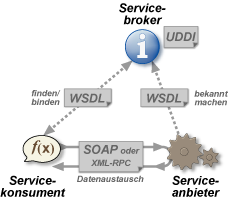
\includegraphics{bilder/Webservice.png}
		\caption{Kontrollfluss eines BPEL Prozesses}
	\label{fig:ExamlpleBPELProzess}
\end{figure}

Bei Web Services handelt es sich nicht um eine bestimmte Technik, sondern um ein B�ndel von verschiedenen Standards und Spezifikationen.
Web Service Stack ...

Bild

Im n�chsten Abschnitt wird WSDL etwas genauer vorgestellt.


\section{WSDL}
Die Beschreibung enth�lt Informationen dar�ber , woraus der Web Service besteht, welche Daten ausgetauscht werden und wie der Web Service aufgebaut ist.
WSDL dient dem Webservice dazu, standardisiertbekannzugeben, welche Funktionen er besitzt, wie die Schnittstellen (Parameter) aussehen und �ber welche Protokolle Konsumenten ihn ansprechen k�nnen.
 Seit M�rz 2001 ist die Version 1.1 aktuell. Auch hier wurde eine Arbeitsgruppe im W3C zur
Weiterentwicklung gegr�ndet, WSDL 1.2 und 2.0 sind in Arbeit.
Versionen 


Damit das Format hinsichtlich zuk�nftiger Nachrichtenformate und Transportprotokolle erweiterbar
ist, gliedert es sich in zwei Teile. Eine abstrakte und eine konkrete Definition.
Die abstrakte Definition beschreibt die Datentypen, die Operationen und Nachrichten. Diese
werden zu so genannten portTypes zusammen gefasst.
Die konkrete Definition bindet die portTypes an ein Transportprotokoll und fasst diese
ports zu services zusammen.
Dokument Struktur
Abstrakte Definition Konkrete Definitionen
Operationen undMessageswerden erstabstrakt beschrieben und dannan das jeweilige Netzwerk-Protokoll undMessage-Format gebunden (SOAP, HTTP, MIME)
Bild

definitions ist das Wurzelelement des WSDL-Dokuments. Es enth�lt den Namen des Services, Namespaces f�r den Service selbst und f�r die verwendete Standards.

types enth�lt Definitionen f�r eigene Datentypen. Standardm��ig werden die Datentypen aus der XML-Schema-Spezifikation verwendet.
Datentypen dienen derInteroperabilit�tvon Anwendungen und Diensten, um eine gemeinsame Austauschbasis f�r Daten zu gew�hrleisten

Das Konzept der XML-Schemas ist
plattformneutralundsprachunabh�ngig
Die Flexibilit�tder XML-Schemas erlaubt es in WSDL die Besonderheiten bestehender Programmiersprachen oder Datenaustauschstandards abzubilden


message  fasst die definierten Typen zu abstrakten Nachrichten zusammen
definiert nur unidirektionale Nachrichten

portType Der portType beschreibt die Schnittstelle des Services. In ihm werden eine oder mehrere
Operationen zusammen gefasst, �hnlich wie ein Java Interface. Diese ordnen der Operation
die Ein- und Ausgabeparameter zu. �ber diese Zuordnung wird das sogenannte Message
Exchange Pattern der Schnittstelle festgelegt.

binding die vom Web Service verwendeten Kommunikationsprotokolle und Nachrichten formate. definiert konkrete Nachrichtenformate und Protokoll-Einzelheiten
Die meist benutzten Protokolle sind SOAP, HTTP GET/POST. 
Eine Bindung muss exakt ein Protokoll spezifizieren. 
Jede Bindung baut auf genau eine Port Type auf.


service definiert die Endpunkte eines Dienstes. Der Endpunkt selbst steht mit einer URI im untergeordneten port-Element. 
Das service-Element stellt aus einem oder mehreren ports einen Dienst zusammen.
Ein port ordnet dem Binding einen bestimmten Endpunkt zu. Wie dieser definiert wird,
h�ngt von dem verwendeten Transportprotokoll ab. Bei SOAP �ber HTTP ist dies beispielsweise
die URL, �ber die der Service Provider erreichbar ist.






  
  
  WSDL ist jedoch nicht allein an SOAP gebunden. Es gibt eine Vielzahl von vordefinierten Bindungen, zu denen auch SOAP 1.1 z�hlt. WSDL h�lt sich an eine abstrakte Beschreibung von Web Services. WSDL verfolgt somit unterschiedliche Ziele:

		
 	Jeder Web-Service l�a�t sich als Objekt verstehen, das verschiedene Methoden
zur Verf�ugung stellt, auf die zugegriffen werden kann. Um diese Zugriffe zu
erm�oglichen und zu automatisieren, ist eine standardisierte Beschreibung der
Schnittstelle zum Web-Service notwendig. Hierf�ur wird die Web-Service Description
Language verwendet.
WSDL ist eine XML-basierte Sprache zur Beschreibung von Web-Services.
Sie beschreibt die Methodenschnittstelle desWeb-Services, nicht aber denWeb-
Service selbst. Neben der Methodenspezifikation beinhaltet sie auch technische
Daten, wie die eigentliche Lage des Dienstes und an welche Transportprotokolle
er gebunden ist.
DieWeiterentwicklung von WSDL wird durch das W3C kooridiniert. WSDL
liegt aktuell in der Version 2.0 vor und gliedert sich in drei Teile.
Die Core Language ([WSDL Pt. 1]) mit allen wesentlichen Strukturierungselementen,
die Message Exchange Patterns ([WSDL Pt. 1]) mit der Definition der
m�oglichen Kommunikationsmuster und
die Bindings, welche den Zugriff auf Operationen und den Transport der
gesendeten Nachrichten beschreiben.

Die Elemente in einem WSDL-Dokument lassen sich in abstrakte Definitionen
und konkrete technische Beschreibungen zu diesen Definitionen unterteilen. Die
abstrakten Elemente dienen dabei der detaillierten Beschreibung der Schnittstelle
einer Softwarekomponente. Die technischen Elemente dagegen beschreiben,
wo Endpunkte der Komponente im Netzwerk lokalisiert und �uber welche
Protokolle sie angesprochen werden k�onnen.
Die Unterscheidung in abstrakte und konkrete Definitionen bedeutet dabei
aus Sicht der Middleware eine Trennung zwischen Schnittstellenbeschreibung
und Serialisierungs- und Transportdetails. Sie erh�oht die Erweiterbarkeit, Wiederverwendbarkeit
und Portabilit�at von Web-Services.
Die konkreten Definitionen referenzieren
dabei stets abstrakte Definitionen. Das bedeutet, da� zu einer abstrakten
Definition mehrere konkrete Implementierungen existieren k�onnen.
Abbildung 6 zeigt die allgemeine Struktur eines WSDL-Dokuments und
die Verkn�upfungen der einzelnen Teilkomponenten. Jedes WSDL-Dokument
wird von einem definitions-Element eingeleitet. Das Element definiert den
Namensraum des WSDL-Dokuments und �offnet alle weiteren ben�otigten Namensr
�aume.
Abstrakte Definition
Die abstrakte Definition beinhaltet die sprach- und plattformunabh�angige Beschreibung
der Schnittstelle des Web-Service. Zu den abstrakten Definitionen
z�ahlen die types- und interface-Elemente.
Innerhalb des types-Elements werden die verwendeten Typen definiert. 
Der konkrete Definitionsteil beinhaltet, an welcher Stelle ein Web-Service �uberhaupt
zu finden und durch welche Transportmechanismen er abrufbar ist. Die
Definition umfa�t die binding- und service-Elemente.
Das binding-Element ist ein Container f�ur Elemente zur Beschreibung der konkreten
Serialisierungs- und Transportdetails f�ur ein deklariertes Interface.





\section{Komposition der Services mit BPEL}
WS-BPEL(kurz BPEL) ist eine XML-basierte, ausf�hrbare Sprache zur Modellierung und Beschreibung
von Gesch�ftsprozessen. BPEL ist 2002 aus IBMs WSFL und Microsofts XLANG entstanden und liegt aktuell in der Version 2.0  als OASIS Standard vor. Durch breite Produktunterst�tzung ist die Sprache auf dem Weg, sich auch als Industriestandard zu etabliert.


Mit BPEL l�sst sich ein Prozess beschreiben, der verschiedene Web Services zu einer Gesamtanwendung verkn�pft. Services k�nnen dabei auf zwei Arten kombiniert werden:
\begin{itemize}
	\item \textbf{Orchestration:} Ein zentraler Prozess koordiniert die
Operationen der Web Services, die in den Prozess
eingebunden sind.
\item \textbf{Choreography:} Es gibt keinen zentralen Koordinator. Jeder in
die Choreography eingebundene Web Service kennt seine Interaktionspartner. Bei der Choreographie erfolgt
die Zusammenarbeit �ber den Austausch von Nachrichten
in einem �ffentlichen Prozess.
\end{itemize}

BPEL unterst�tzt Orchestration und Choreography durch
\begin{itemize}
	\item \textbf{Executable Processes:} Spezifikation des intenen Verahaltens eines
Ge\-sch�fts\-pro\-zesses, der durch eine Engine
ausgef�hrt werden kann. Enth�lt alle f�r die Pro\-zess\-aus\-f�h\-rung notwendige Informationen bis auf die tats�chlichen Endpunkte der Web Services.
\item \textbf{Abstract Business Processes:} Spezifikation des
Nachrichtenaustauschs zwischen Partnern. Beschreibung des nach au�en sichtbaren Verhaltens des Prozesses. Keine Aussagen �ber interne Logik.
\end{itemize}

W�hrend abstrakte Prozesse nur der Beschreibung des Prozessverhaltens dienen,  k�nnen aus\-f�hr\-ba\-re BPEL-Prozesse (\textit{executable Processes}), wie der Name schon sagt, in einer BPEL-Engine ausgef�hrt werden. Da der Kontext dieser Arbeit das Testen von BPEL-Prozessen ist, und das Testen die Ausf�hrung voraussetzt, sind dementsprechend auch nur die ausf�hrbaren Prozesse relevant. Die weiteren Betrachtungen in dieser Arbeit beschr�nken sich aus diesem Grund ausschlie�lich auf die ausf�hrbaren Prozesse.


Mit BPEL k�nnen langlebige und zustandsbehaftete Prozesse modelliert werden. Es ist dabei m�glich, eine sehr flexible Fehlerbehandlung mit Kompensationsm�glichkeiten zu realisieren. Durch die strikte Trennung der Ablauflogik (BPEL-Prozess) und Implementierung (einzelnen Web Services) ist die Anpassung bei �nderungen des zugeh�rigen Gesch�ftsprozesses einfach durchzuf�hren. Bei ausreichend kleiner Granularit�t der einzelnen Services betreffen die Auswirkungen einer Gesch�ftsprozess�nderung ausschlie�lich den BPEL-Prozess selbst.

Die Schnittstelle nach au�en eines BPEL-Prozesses wird ebenfalls in WSDL beschrieben und kann wiederum als Web Service in andere Prozesse eingebunden werden.
Die damit gegebene Rekursivit�t erm�glicht durch hierarchische Aufbau der Prozessen die Abstraktionsschichten einzuf�hren und damit die Komplexit�t besser zu beherrschen.

Allerdings bring BPEL auch einige Nachteile mit sich. Als Erstes ist die Komplexit�t der Sprache zu nennen. Jedoch ist diese Komplexit�t in dem Anspruch begr�ndet, jede Art von Gesch�ftsprozessen realisieren zu k�nnen und zwar quer zu allen IT-Plattformen. Auch zu nennen sind die redundanten Ausdrucksmittel der Sprache, die aufgrund der Vereinigung zwei Sprachen entstanden sind, und oft das Verst�ndnis der Prozessen erschweren. Als letztes ist noch das Fehlen einer standardisierten grafischen Notation zu erw�hnen.

In den folgenden Abschnitten wird auf einige f�r diese Arbeit relevanten Aspekte der BPEL eingegangen.

\subsection{Partners}

BPEL-Prozesse interagieren mit anderen Web Services, die
man als Partner oder Partner-Prozesse bezeichnet. Ein
BPEL-Prozess benutzt Dienste von Partnern und bietet selbst Dienste nach au�en an. Die Beziehung zwischen den m�glichen Partner und dem Prozess selbst wird zuerst abstrakt durch die Rollen in einem \textit{Partner Link Type} beschrieben. In jedem solchen Element werden mindestens eine und maximal zwei Rollen definiert. Die Rollen k�nnen dabei entweder vom Prozess oder vom Partner �bernommen werden.  Derjenige der diese Rolle �bernimmt muss den \textit{Port Type}, der zu der Rolle zugeordnet ist, in seiner WSDL-Schnittstelle anbieten.

Die Beziehung zwischen dem BPEL-Prozess und einem konkreten Partner wird letztendlich in \textit{Partner Link} durch die Zuweisung der Rollen definiert.
Die Bindung an einen konkreten Web Service kann entweder statisch zum Zeitpunkt des Deployments oder dynamisch zur Laufzeit erfolgen. Die Abbildung \ref{fig:partnerLink} stellt den Zusammenhang grafisch dar.
\begin{figure}[htbp]
	\centering
		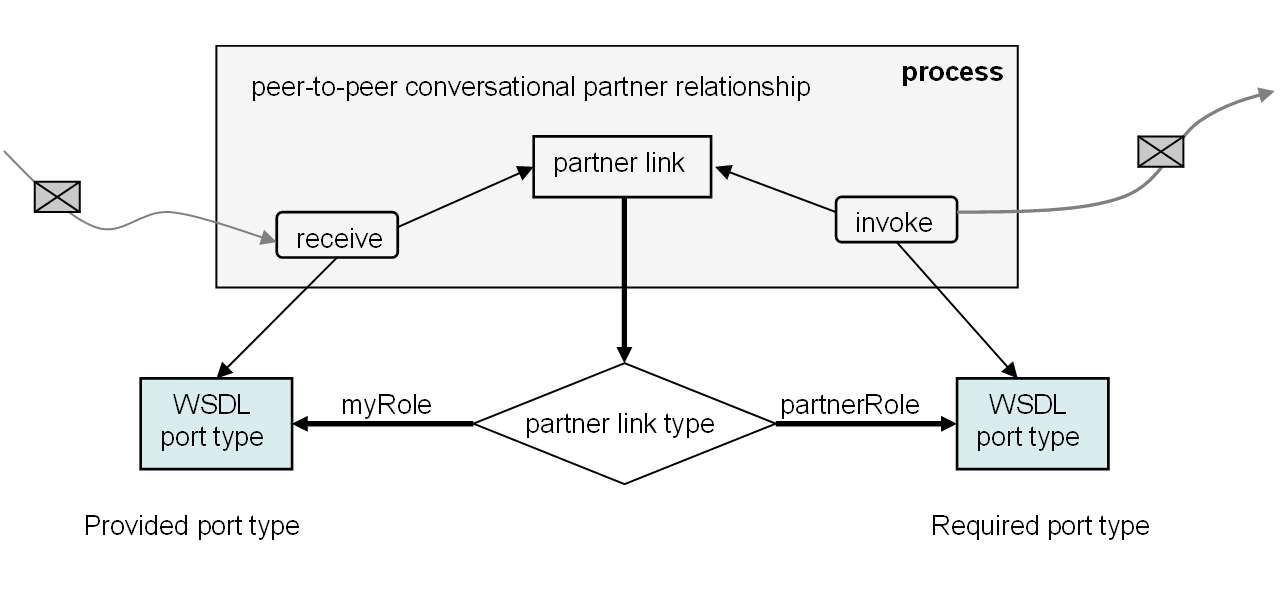
\includegraphics[width=0.82\textwidth]{bilder/partnerLink.png}
		\caption{Partner Link\cite{Dieter}}
	\label{fig:partnerLink}
\end{figure}

\subsection{BPEL Prozess}
BPEL-Prozess ist definiert in Form eines XML-Dokuments. Die Wurzel eines BPEL-Dokuments ist das Element $<$process$>$, welches die Struktur und den
Kontrollfluss eines Gesch�ftsprozesses in sich kapselt. Das Prozess-Element enth�lt drei wichtige Abschnitte:

\begin{itemize}
	\item $<$partnerLinks$>$ - Partner Link-Definitionen, die f�r Kommunikation mit den Partner benutzt werden.   
	\item $<$variables$>$ -  Variablen f�r die Speicherung von internen Daten und Daten, die Empfangen oder Gesendet werden.  Alle in diesem Bereich definierten Variablen sind globale Variablen. Es gibt M�glichkeit lokale Variablen zu definieren. Sie werden in einem Sichtbarkeitsbereich
(Scope) durch einen eindeutigen Namen und einen Datentyp definiert. 
	\item $<$activity$>$ - Gesch�ftslogik in Form von Aktivit�ten. 
\end{itemize}
 
Die Gesch�ftslogik wird in BPEL durch so genannte Aktivit�ten realisiert. Es gibt zwei Arten von Aktivit�ten: Basisaktivit�ten (basic activities) und Strukturierte Aktivit�ten (structured activities). Basisaktivit�ten beschreiben die elementaren Schritte des Prozesses. Strukturierten Aktivit�ten bestimmen den Kontrollfluss und k�nnen deswegen weitere Basis- oder Strukturierten Aktivit�ten enthalten. 

Die Basisaktivit�ten repr�sentieren einzelne Aktionen:
\begin{itemize}
\item $<$invoke$>$ - Aufruf anderer Web Services aus dem Prozess heraus. 
\item $<$receive$>$ - Blockierendes Warten auf Nachrichten.
\item $<$reply$>$ - Versenden einer Antwort.
\item $<$assign$>$ - Zuweisung und Manipulation von Variablenwerten.
\item $<$throw$>$ - Explizites Signalisieren eines Fehlers, welcher durch Fehlerbehandlungen abgefangen werden kann.
\item $<$exit$>$ - Beenden einer Prozessinstanz.
\item $<$wait$>$ - Warten auf einen Zeitpunkt oder f�r eine Zeitspanne.
\item $<$empty$>$ - Nichts machen (NOP).
\item $<$compensate$>$ - Kompensation aller eingebetteten Scopes, $<$compensate$>$ kann nur im FaultHandler
oder CompensationHandler eingebettet sein.
\item $<$compensateScope$>$ - Kompensation
eines speziellen Scope.
\item $<$rethrow$>$ - Wieterreichen der abgefangenen Fehler.
\item $<$validate$>$ - Validierung der Variablenwerten gegen XML-Schema.
	\end{itemize}
Mit den ersten drei lassen sich alle Kommunikationsszenarien implementieren:
\begin{itemize}
	\item synchrone request\slash response-Kommunikation
	\item asynchrone request\slash response-Kommunikation
	\item \textit{one way}-Kommunikation
\end{itemize}

WS-BPEL beschreibt den Ablauf von Gesch�ftsprozessen als strukturierte Aktivit�ten:
\begin{itemize}
\item $<$sequence$>$ - sequentielle Ausf�hrung von Aktivit�ten
\item $<$if$>$ - bedingte Auf�hrung von Aktivit�ten.\textit{ if}-Aktivit�t besitzt mehrere geordnete Bedingte Zweige definiert  durch $<$\textit{if}$>$- und $<$\textit{elseif}$>$- Elemente gefolgt von einem optionalem $<$\textit{else}$>$-Element. Der erste Zweig mit der zutreffenden Bedingung wird ausgef�hrt. 
\item $<$while$>$ - iterative Ausf�hrung der Aktivit�ten. Die Ausf�hrung findet solange statt, bis die Bedingung nicht mehr erf�llt ist. Die Auswertung der Bedingung findet vor jeder Schleifenausf�hrung statt.
\item $<$repeatUntil$>$ - iterative Ausf�hrung von Aktivit�ten. Die Ausf�hrung findet solange statt, bis die Bedingung erf�llt ist. Die Auswertung der Bedingung findet nach jeder Schleifenausf�hrung statt.
\item $<$forEach$>$ -  Ausf�hrung mehrerer Scopes. Die Ausf�hrung kann entweder seriell oder parallel erfolgen (gesteuert durch Attribut \textit{parallel}).
\item $<$pick$>$ - blockierendes Warten auf  Eintreffen eines von mehreren Ereignissen. Bei dieser strukturierenden Aktivit�t wird ein Zweig aus mehreren anhand eines Ereignisses (Nachricht oder Alarm) ausgew�hlt. Wurde ein zutreffendes Ereignis empfangen, so wird die zugeh�rige Aktivit�t ausgef�hrt und alle nachfolgenden Ereignisse verworfen. 
\item $<$flow$>$ - erm�glicht parallele Ausf�hrung von Aktivit�ten mit Synchronisationsm�glichkeit (siehe Abschnitt \ref{sec:linkkonzept}).  
\end{itemize}



\subsection{Link-Konzept}\label{sec:linkkonzept}
 In einer flow-Aktivit�t k�nnen Links definiert werden. Sie dienen
der Synchronisation nebenl�ufiger Aktivit�ten. Jeder Link verbindet eine
\textit{source}-  mit einer \textit{target}-Aktivit�t und besitzt eine implizite oder explizite \textit{transition condition} (boolscher Ausdruck). Ist der Ausdruck nicht spezifiziert, so ist der Wert der \textit{transition condition} \textit{true}. Jede Aktivit�t, die das Ziel eines Links ist, hat eine implizite oder explizite \textit{join condition} (boolscher Ausdruck). Im impiziten Fall ist das eine ODER-Verkn�pfung der Status aller eingehenden Links. Die Auswertung dieser Bedingungen bei der Ausf�hrung wird an einem kleinem Beispiel erl�utert.

\begin{figure}[h!]
	\centering
		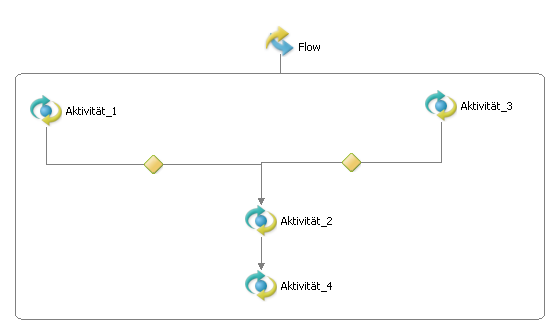
\includegraphics[width=0.53\textwidth]{bilder/FlowBespielLinks.png}
	\caption{Beispiel einer flow-Aktivit�t mit Synchronisationslinks}
	\label{}
\end{figure}

Ist die Ausf�hrung der Aktivit�t \textit{activity\_1} beendet, so wird \textit{transition condition} des Links \textit{link\_1} ausgewertet und der Status auf den entsprechenden Wert \textit{true} oder \textit{false}  gesetzt. Auf dieselbe Weise wird der Status des zweiten Links ermittelt. Stehen die Status der beiden Links fest, so kann die \textit{join condition} der Aktivit�t \textit{activity\_3} ausgewertet werden. Bei einem \textit{true}-Wert wird die Ausf�hrung des Prozesses  ganz normal mit \textit{activity\_3}  fortgesetzt. Ist der Wert \textit{false}, so wird eine Fehlermeldung (\textit{Join Failure}) erzeugt und der Kontrollfluss f�r Fehlerbehandlung aktiviert. Ist dieses Verhalten unerw�nscht, so kann das Standardattribut \textit{suppressJoinFailure} auf den Wert \textit{"`yes"'} gesetzt. In diesem Fall wird \textit{activity\_3} ebenfalls nicht ausgef�hrt, allerdings wird der Prozess ganz normal, ohne eine Fehelermeldung zu produzieren, mit der \textit{activity\_4} fortgesetzt.

Ist \textit{activity\_2} zum Beispiel in einem \textit{if}-Zweig, der w�hrend der Ausf�hrung nicht aktiviert wird, so kann der Status des ausgehenden Links nicht auf die normale Weise ermittelt werden. Die \textit{join condition}  kann ohne des Status des zweiten Links nicht ausgewertet werden.  Das w�rde zu einer Blockierung des Kontrollflusses bei \textit{activity\_3} f�hren. F�r solche Situationen sieht BPEL \textit{Dead-Path-Elimination} vor. Wird eine Aktivit�t aufgrund einer zu
\textit{false} ausgewerteten \textit{join condition}
oder eines nicht abgearbeiteten Zweiges einer if- oder pick-Aktivit�t nicht
ausgef�hrt, so wird f�r alle eventuell vorhandenen ausgehenden Links die \textit{transition condition}
auf \textit{false} gesetzt. Diese Werte werden soweit wie m�glich entlang des Pfades propagiert. Auf die Weise werden Pfade eliminiert, die nicht zur Ausf�hrung kommen, und damit Blockierungen des Kontrollflusses vermieden.

Bei der Verwendung von Links ist folgendes zu beachten:
\begin{itemize}\label{restrictions}
	\item ein Link darf genau eine \textit{source} und eine \textit{target}-Aktivit�t verbinden,
	\item Links d�rfen keine Zyklen bilden,
	\item es m�ssen \textit{boundary crossing}-Restriktionen beachtet werden:
\begin{itemize}
	\item Links d�rfen nicht in oder aus den Wiederholungsschleifen und \textit{Compensation Handler} ein- bzw. austreten
	\item Links d�rfen aus den \textit{Fault} und \textit{Termination Handler} nur austreten
	\item Links, die aus den \textit{catch} oder \textit{catchAll}-Bl�cken des Fault Handlers oder aus dem Termination Handler austreten, m�ssen in einem nicht zu den Handlern zugeh�rigem \textit{Scope} landen.)
\end{itemize}
\end{itemize}

\subsection{\textit{Scope}}
\textit{Scopes} dienen zur Strukturierung von BPEL-Prozessen und definieren Sichtbarkeitsbereiche f�r Variablen und Ereignisse. Ein \textit{Scope} ist ein Ausfuhrungskontext f�r Aktivit�ten mit der M�glichkeit,  eigene Fault, Compensation, Termination und Event Handler zu definieren. Das $<$process$>$-Element ist ein impliziter globaler Scope (Prozess-Scope).
\subsubsection{\textit{Event Handler}}
 BPEL bietet die M�glichkeit, parallel zum normalen Kontrollfluss bestimmte Ereignisse
mit so genannten \textit{Event Handlern} zu behandeln. \textit{Event Handler} geh�ren zu einem
bestimmten \textit{Scope} innerhalb des Prozesses oder zu dem globalen Prozess \textit{Scope}.
Sie behandeln Ereignisse, die den zugeordneten G�ltigkeitsbereich betreffen.
Innerhalb eines \textit{Event Handlers} k�nnen beliebige Abfolgen von BPEL Aktivit�ten definiert
werden. Es gibt zwei Typen von Ereignissen, auf die in einem \textit{Event Handler} reagiert werden kann: Nachrichten und zeit gesteuerten Ereignisse.

\subsubsection{Fehlerbehandlung und Kompensation}
  BPEL-Sprache hat wie viele moderne Programmiersprachen ein Konzept zur strukturierten Behandlung von Laufzeitfehlern.
  Tritt ein Fehler im laufenden Prozess auf, so wird ein f�r diesen Bereich zust�ndiger \textit{Fault Handler} aufgerufen. 
  Oft m�ssen im Fehlerfall bereits abgeschlossene Aktivit�ten kompensiert werden. In BPEL kann
daf�r ein \textit{Compensation Handler} definiert werden, in dem Aktivit�ten f�r die Kompensation festgelegt werden.
\textit{Compensation Handler} k�nnen nur aus \textit{Fault Handler} oder \textit{Compensation Handler} des umschlie�enden \textit{Scopes} aufgerufen werden. Au�erdem ein \textit{Compensation Handler} kann nur f�r \textit{Scopes} aufgerufen werden, die
ordnungsgem�� abgearbeitet wurden. Jedes \textit{Scope} besitz ein Fault und \textit{Compensation Handler}, der Prozess selbst hat in BPEL 2.0 nur den \textit{Fault Handler}. 
  
Ist kein benutzerdefiniertes \textit{Fault Handler} spezifiziert, so gibt es ein impliziter \textit{Fault Handler}, der die \textit{Compensation Handler}
aller direkt eingeschlossener \textit{Scopes} in der umgekehrten Reihenfolge ihrer Abarbeitung aufruft und
anschlie�end den Fehler an den umschlie�enden Scope oder den Prozess selbst weiter reicht. Es k�nnen eigene \textit{Fault Handler} spezifiziert werden, der
je nach Art des auftretenden Fehlers eine bestimmte BPEL-Aktivit�t ausf�hrt. F�r die Bindung bestimmter Aktivit�ten an die bestimmten Fehler werden \textit{catch} und \textit{catchAll}-Elemente verwendet.
  
Die Fehler k�nnen auch in den \textit{Compensation} und in den \textit{Fault Handler} selbst auftreten. In die Abbildung \ref{fig:ScopeFaultCompensation2} wird der Zusammenhang zwischen \textit{Handler} und \textit{Scopes} grafisch dargestellt. Die Pfeile zeigen dabei den m�glichen Kontrollfluss. 
\begin{figure}[h!]
	\centering
		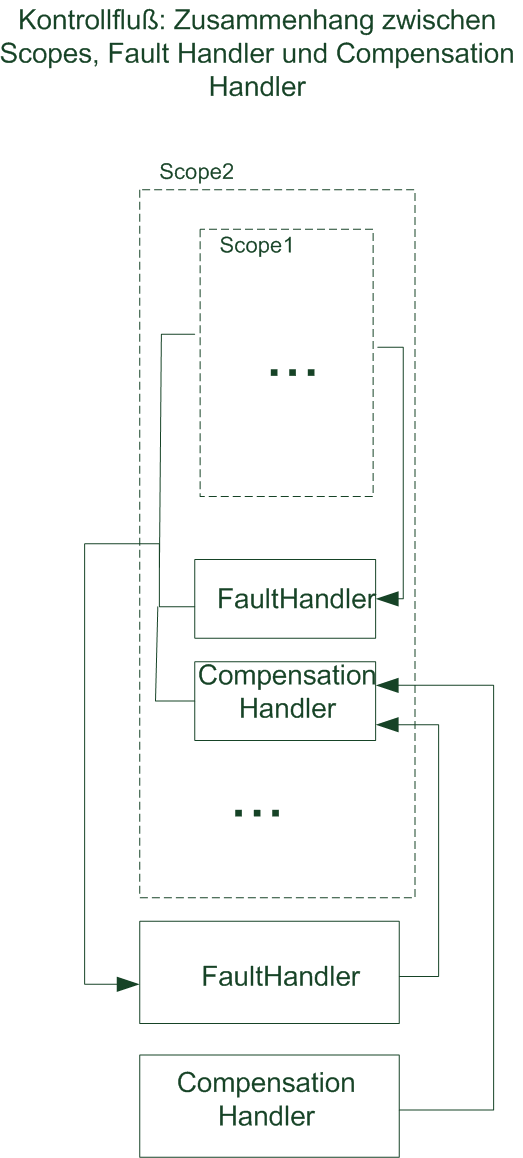
\includegraphics[width=0.33\textwidth]{bilder/ScopeFaultCompensation2.png}
	\caption{Zusammenhang zwischen Scopes, Fault und Compensation Handler}
	\label{fig:ScopeFaultCompensation2}
\end{figure}

 Als einzige Ausnahme bietet \textit{invoke}-Aktivit�t die M�glichkeit, eigene \textit{Fault} und \textit{Compensation Handler} zu definieren. Es entspricht einem expliziten \textit{Scope}, das die \textit{invoke}-Aktivit�t umschlie�t und \textit{Compensation} und \textit{Fault Handler} besitzt.

\subsubsection{Termination Handler}
Scopes besitzen die M�glichkeit, auf den Ablauf einer erzwungenen Terminierung Einfluss zu
nehmen. Das Verhalten wird innerhalb eines Termination Handler festgelegt, der im Falle einer erzwungenen Terminierung nach der
Beendigung aller laufenden Aktivit�ten des Scope ausgef�hrt wird. Ist kein
Termination Handler definiert, wird ein Standard-Termination-Handler aktiviert. Dieser kompensiert
alle erfolgreich beendeten eingebetteten Scopes in der umgekehrten Ausf�hrungsreihenfolge. Er verh�lt sich also wie der Standard-Fault-Handler.

\subsection{Prozessinstance}
Die Erzeugung von Prozessinstanzen erfolgt implizit anhand von Aktivit�ten (\textit{receive} oder \textit{pick}),
beim Eintreffen von externen Nachrichten. Die entsprechenden Aktivit�ten werden mit dem Attribut \textit{createInstance}=\textit{"'yes"'} gekennzeichnet.  
Zur
Identifikation von laufenden Prozessinstanzen dienen so genannten \textit{Correlation Sets}. Diese werden von BPEL-Engine verwendet, um Nachrichten an richtige Instanzen weiterleiten zu k�nnen.

Prozessinstanzen werden beendet, wenn die Aktivit�ten, die das Verhalten von Prozessen bestimmen,
abgearbeitet wurden (normale Beendigung), wenn ein Fehler den Prozess-\textit{Scope} erreicht,
der entweder behandelt oder nicht behandelt wird, oder wenn von Prozessinstanzen die \textit{exit}-
Aktivit�t ausgef�hrt wurde.


   

\subsection{Engine}
Ein BPEL-Prozess besteht aus der Gesch�ftslogik (definiert in BPEL), Servicebeschreibung (WSDL) und optional aus weiteren Datentypen (XML Schema). Diese Informationen werden zusammengefasst und in eine BPEL Engine deployt. Die Engine ist unter anderem daf�r verantwortlich, die \textit{Endpoints} der Partner des BPEL Prozesses zu spezifizieren. F�r jeden Link muss bekannt sein, welche WSDL-service und -port und welche Adresse f�r die Kommunikation benutzt werden sollen. Diese Information wird in so genannten \textit{Deployment Descriptoren} festgelegt.

\textbf{ActiveBPEL Engine}.
Die ActiveBPEL-Engine ist eine Runtime-Umgebung f�r die Business Process Execution Language, die in Java implementiert und sowohl BPEL 1.1 als auch BPEL2.0 konform ist. 
Die Engine l�uft innerhalb des Apache Tomcat Servers und stellt dort die zum automatischen Gesch�ftsprozess zusammengefassten Web Services - wiederum als Web Service - zur Verf�gung. Zum Deployen wird eine Archivdatei, die das BPEL-Modell, WSDLDateien
und den Engine-spezifischen Deployment Descriptor enth�lt, in das bpr-Verzeichnis
des Servers, auf dem die ActiveBPEL-Engine l�uft, abgelegt. 

\section{BPEL Testen}
Eine der wichtigsten Aufgaben bei der
Entwicklung von komplexer, umfangreicher Software ist die Pr�fung. In
der Praxis wird daf�r ein erheblicher Anteil des
gesamten Entwicklungsaufwands aufgebracht. Es
existieren zahlreiche Methoden und Techniken f�r die
Pr�fung von Software. Testen ist ein in der konventionellen Softwareentwicklung unentbehrliches Mittel zur Qualit�tssicherung.

\textit{Testen ist ein Prozess, ein Programm mit der Absicht
auszuf�hren, Fehler zu finden.}

Beim Testen von BPEL-Prozessen m�ssen im Vergleich zu anderen Anwendungen eine Besonderheit beachtet werden: externe Abh�ngigkeit in Form von Web Services. Die Durchf�hrung eines kompletten Tests ist nur dann m�glich, wenn alle beteiligten Web Services erreichbar sind und reproduzierbare Ergebnisse liefern. 
Zum richtigen Problem wird das Testen, wenn externe Service-Anbietern eingebunden sind. In der Regel hat man in dieser Situation nur die Beschreibung der Schnittstelle aber kein Quellcode. Aus diesem Grund kann ein Web Service in einer Testumgebung repliziert werden. 
Ein weiteres Problem ist das Testen von Fehlersituationen. Daf�r m�ssen die solche Situationen, wie "`Web Service nicht erreichbar"' oder "`antwortet mit einer Fehlermeldung"' simuliert werden. \cite{LuebketestSOA} 

Die angestrebte Isolation des BPEL-Prozesses f�r das Testen kann mit Hilfe eines Unit-Tests erreicht werden. Im Rahmen einer Masterarbeit \cite{Mayer2006}  ist das BPELUnit-Framework entstanden, der das Testen von BPEL-Kompositionen in isolation erm�glicht.

\subsection{BPELUnit-Framework}
BPELUnit ist ein Framework zum Testen von BPEL-Kompositionen in Isolation. Es erm�glicht wiederholbare \textit{white-box}-Tests zu erstellen, zu speichern und auszuf�hren. 
Das Framework richtet sich prim�r an die Entwickler, die das Testen und Programmieren w�hrend des Entwicklungsprozesses abwechseln machen. 
Dementsprechend bietet das  Framework eine schnelle und einfache M�glichkeit, die erstellten Tests immer wieder auszuf�hren und Ergebnisse auszuwerten.
Der Kern ist unabh�ngig von der Pr�sentationsschicht implementiert und bietet eine Schnittstelle f�r die Implementierung der Clients an. Drei Clients geh�ren geh�ren zum Framework:
\begin{itemize}
	\item Befehlszeilen-Client 
	\item ANT-Integration 
		\item Eclipse-Plugin 
\end{itemize}
 Bei den ersten beiden Clients erfolgt die Konfiguration �ber XML-Dokumente, die im Konfigurationsverzechnis (\textit{conf}) der BPELUnit-Installation abgelegt sind. Eclipse-Plugin erm�glicht neben der grafischen Darstellung des Ergebnisses auch komfortable Erstellung der Tests mit Hilfe eines Editors.
 
 Das Framework unterst�tzt \textit{ActiveBPEL Engine} und \textit{Oracle BPEL Process Manager (Server)}. Weitere Engines k�nnen durch implementieren entsprechenden Adapter integriert werden.

BPELUnit isoliert den zu testenden Prozess, indem es die Partner des Prozesses durch Mock's ersetzt, die diese Partner simulieren. Dadurch k�nnen Abh�ngigkeiten von externen Services aufgel�st werden. Schnellere Tests ist der angenehme Nebeneffekt dieser Vorgehensweise, denn die Simulationen der Web Services meist schneller als reale Implementierungen sind. 

\textbf{BPELUnit-Architektur}. Das Framework basiert auf einer Schichtarchitektur, die in der Abbildung \ref{fig:schichtarchitektur} dargestellt ist. 
 Der erste von unten Schicht ist f�r die Testspezifikation zust�ndig und legt fest, wie die Testdaten und das Verhalten der Partner definiert werden. Die Tests werden in den Test Suiten organisiert, wof�r die \textit{Test Organization}-Schicht verantwortlich ist. Die Ausf�hrung der Tests wird in der dritten Schicht \textit{Test Execution} realisiert. \textit{Test Results}-Schicht sorgt f�r die Sammlung der Daten und Statistiken  w�hrend der Tests.  Im folgenden werden die einzelnen Schichten etwas n�her erl�utert.
 \begin{figure}[htbp]
	\centering
		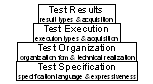
\includegraphics[width=0.47\textwidth]{bilder/FrameworkLayer.png}
		\caption{Schichtarchitektur des BPELUnit-Frameworks}
	\label{fig:schichtarchitektur}
\end{figure}
  
 
 \textbf{Testspezifikation}.
 Ein BPEL-Prozess hat einen Client und beliebige Anzahl von Partner. Die Partner bzw. die Web Services laufen parallel ab und interagieren dabei mit dem BPEL-Prozess. 
Das Verhalten der Partner (Mock's) w�hrend der Tests wird in den so genannten Testf�llen (\textit{eng. Testcases}) definiert. Zu diesem Zweck werden f�r jeden Testfall so genannten \textit{Tracks} definiert: einen \textit{Client-Track} und beliebig viele \textsl{Partner-Tracks}. Die Tracks legen die Interaktionen der jeweiligen Partner mit dem BPEL-Prozess anhand von Sequenzen der atomaren Interaktionen (Aktivit�ten) fest..
Dabei werden folgende Interaktionsmuster unterst�tzt: 
\begin{itemize}
	\item \textit{one way}-Interaktion: \textit{receive} oder \textit{reply},
	\item synchrone \textit{two way}-Interaktion: \textit{receive-reply} und \textit{reply-receive},
	\item asynchrone \textit{two way}-Interaktion: \textit{receive-reply} und \textit{reply-receive}.
\end{itemize}


 \begin{figure}[htbp]
	\centering
		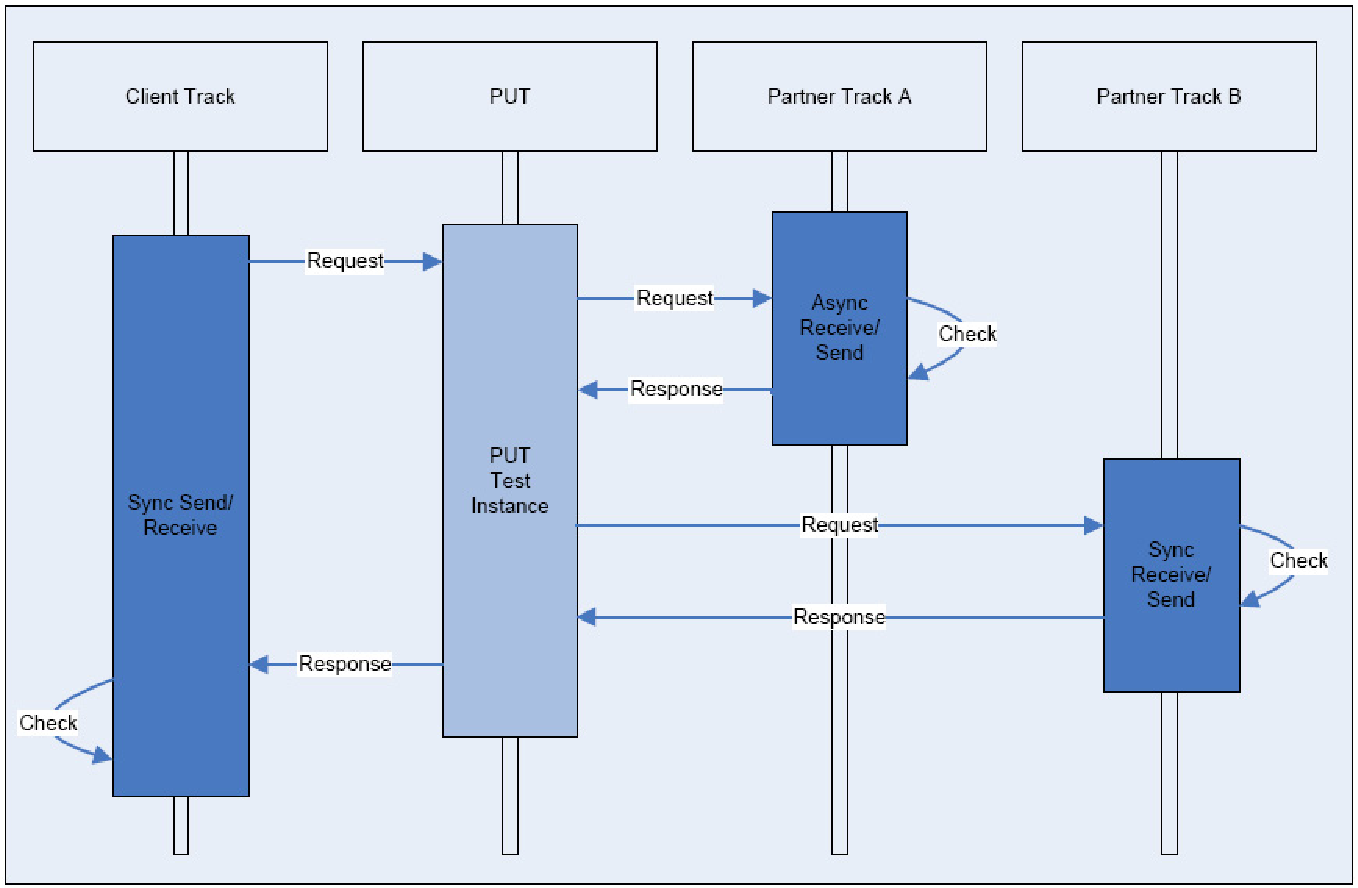
\includegraphics[width=0.8\textwidth]{bilder/TestcaseSequence.pdf}
		\caption{BPELUnit - Sequenzen in einem Testfall}
	\label{fig:sequenzen}
\end{figure}

Die Abbildung \ref{fig:sequenzen} zeigt das Zusammenspiel der Sequenzen eines Testfalls.

Durch Daten, die an den BPEL-Prozess verschickt werden, kann der Prozess gesteuert und bestimmte Zweige des Kontrollflusses stimuliert werden. Das Kenntnis der inneren Struktur ist vorausgesetzt (white-box-Test).
 Die Daten, die bei der Interaktion mit BPEL-Prozess verschickt werden, sind in XML spezifiziert. Es k�nnen WSDL-Nachrichten und sowohl einfache Datentypen als auch Elementen der XML Schema verwendet werden. Die Daten, die der BPEL-Prozess verschickt, k�nnen auf die Korrektheit �berpr�ft werden. 
F�r die Auswahl der relevanten Daten wird XPath \cite{W3C1999} verwendet. 

Mit der F�higkeit des Frameworks, die SOAP Faults zu  empfangen und zu senden, steht dem Tester die M�glichkeit zur Verf�gung, die Fault und Compensation Handler des BPEL-Prozesses zu testen.  
 
 
\textbf{Testorganisation}.  
Die einzelnen Testf�lle werden wie in den konventionellen Programmiersprachen in einer \textit{suite} organisiert. \textit{Suite} referenziert alle f�r den Test notwendigen Elemente: zu testende BPEL-Komposition, WSDL Beschreibungen, XML-Schemata usw. Au�erdem definiert die Suite f�r alle enthaltenen Testf�lle eine globale Testumgebung mit einer \textit{setup} und \textit{shutdown}-Routine, die f�r das \textit{Deployment} und \textit{Undeployment} des Prozesses zust�ndig ist. 

\textbf{Ausf�hrung der Tests}. Zum Testen muss der BPEL-Prozess in einer Testumgebung ausgef�hrt werden, die die Input- und Output-Daten des BPEL-Prozesses entsprechend der Testspezifikation behandelt. \textit{Real-life}-Testen hei�t der Ansatz, der bei BPELUnit-Framework daf�r verwendet wird. Dabei wird der zu testende BPEL-Prozess in eine BPEL-Engine deployt und als Web Service aufgerufen. Die Partner-Web Services m�ssen dabei durch Mock's ersetzt werden, die das Verhalten der Web Services simulieren, d.h., Web Service-Aufrufe empfangen und/oder selbst absetzen.   Beim \textit{Deployen} des BPEL-Prozesses m�ssen alle URI's der Partner-Web Services durch die URI's der Mock's ersetzt werden. 

 \begin{figure}[htbp]
	\centering
		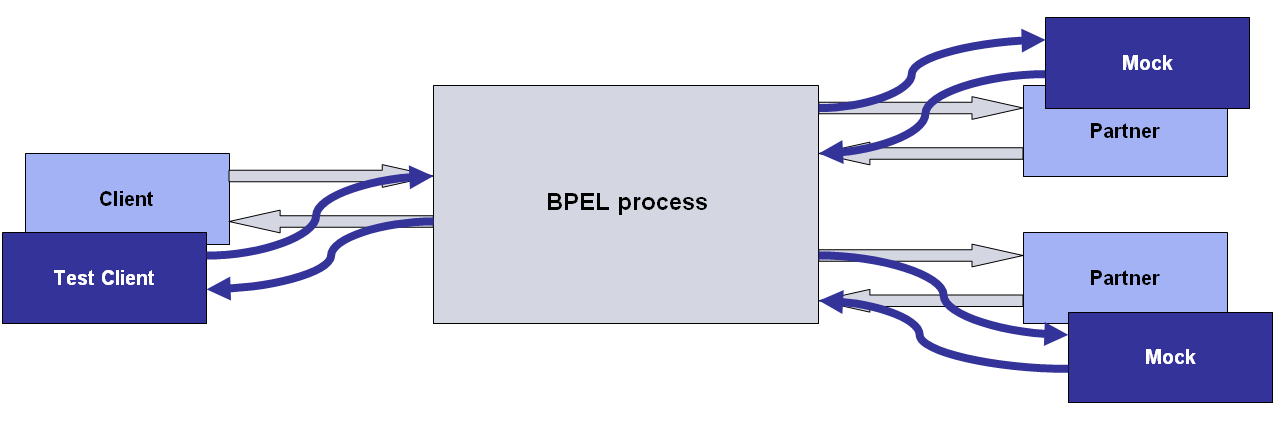
\includegraphics[width=0.75\textwidth]{bilder/BPLEUnitTestHarness.png}
		\caption{BPELUnit -Testumgebung}
	\label{fig:loggingservice}
\end{figure} 

Die Testumgebung ist neben der Simulation der Partner auch f�r die Kommunikation mit dem BPEL-Prozess verantwortlich, die �ber SOAP-Nachrichten stattfinden. Zu diesem Zweck simuliert BPELUnit den kompletten Web Service Stack und kommt mit allen wichtigen SOAP-Konstrukten zu recht. Das Framework erledigt sowohl das Verpacken der Daten in SOAP-Nachrichten als auch dekodieren der empfangenen SOAP-Nachrichten (Abbildung \ref{fig:bpelmiddleware}) und �bernimmt damit dem Tester viel Arbeit.
  
  
 \begin{figure}[htbp]
	\centering
		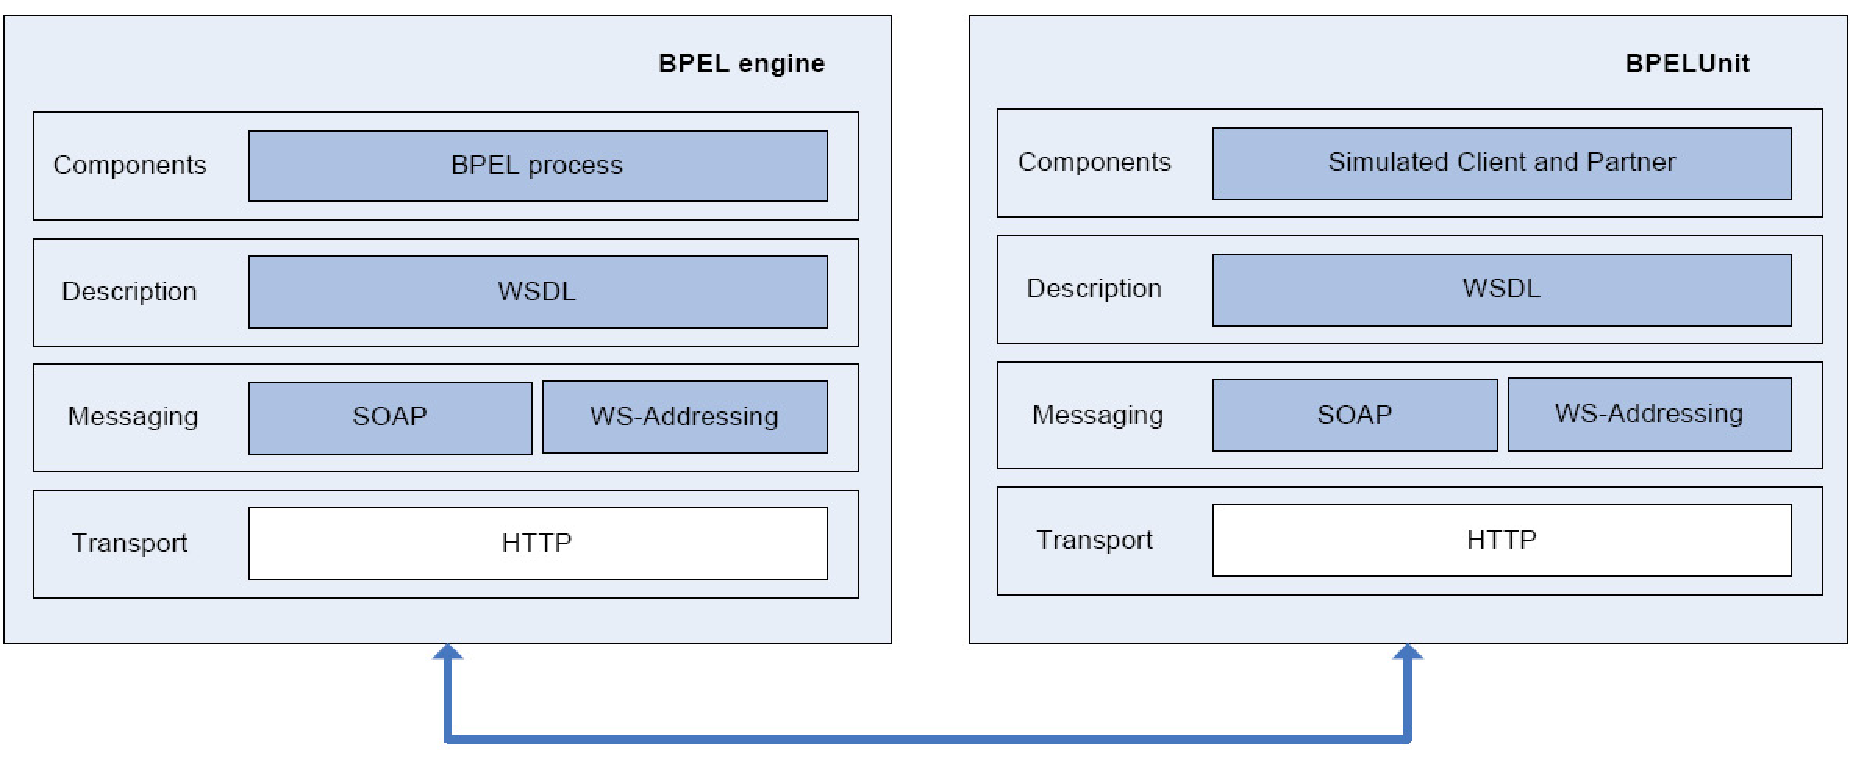
\includegraphics[width=0.98\textwidth]{bilder/BPELUnitMiddleware.pdf}
		\caption{Kommunikation zwischen BPEL-Prozess und simulierten Partnern}
	\label{fig:bpelmiddleware}
\end{figure}


F�r das \textit{Deployment} eines BPEL-Prozesses sind anbieterspezifische \textit{Deployment Descriptoren} erforderlich, die nicht standardisiert sind. Das \textit{Deployen} des BPEL-Prozesses ist, wie bereits erl�utert notwendig, und wird durch BPELUnit automatisch ausgef�hrt. Dazu muss f�r die jeweilige Engine ein entsprechendes Adapter implementiert werden.


\textbf{Testergebnisse}.
Beim Testen wird der BPEL-Prozess in einer Engine ausgef�hrt. Der beschr�nkte Zugriff auf den Prozess (bedingt durch die Ausf�hrung in einer BPEL-Engine) w�hrend der Tests erschwert die Sammlung der Information �ber die Ausf�hrung wesentlich. BPELUnit kann nur berichten, ob der Testfall erfolgreich war oder nicht. Im Fehlerfall 
werden zwei Typen von Fehlern unterschieden:
\begin{itemize}
	\item Fehler auf der Anwendungsebene - zum Beispiel eine erwartete Nachricht von BPEL ist nicht angekommen, oder enth�lt falsche Informationen oder zu viele Nachrichten sind angekommen,
	\item Fehler auf der Kommunikationsebene - Problem mit dem Web Service Stack.
\end{itemize}

Eine wichtige Information beim Testen ist die erreichte Testabdeckung. Das BPELUnit-Framework wird im praktischen Teil mit der Funktionalit�t der Ermittlung von  Testabdeckung erweitert.
 
  

\section{Abdeckung, als Ma� f�r die Testqualit�t}
Um die Softwarequalit�t anhand der Test bewerten zu k�nnen, m�ssen zus�tzliche
Informationen �ber die Tests bekannt sein. Wichtig sind unter anderem die Anforderungs-,
Code- und Datenabdeckung der Tests.
\begin{itemize}
	\item \textbf{Anforderungsabdeckungsmetriken} (\textit{eng. requirements coverage}) ist eine funktionale
Abdeckung auf Basis einer Spezifikation, die angibt, inwieweit die Testf�lle alle Anforderungen abdecken. Diese Metrik wird meist im Zusammenhang mit \textit{Black-Box-Tests} verwendet. 
	\item \textbf{Codeabdeckungsmetriken} (\textit{eng. code coverage}) ist eine Metrik f�r das Verh�ltnis zwischen
zu testenden und tats�chlich getesteten Elementen des Pr�flings. Die Tests, die auf der Codeabdeckung basieren, geh�ren zur Gruppe der strukturorientierten Testtechniken und zielen darauf ab, die innere Struktur der Software zu testen (\textit{White-Box-Test}).\cite{MyersJune2004}
\item \textbf{Datenabdeckungsmetriken} (\textit{eng.data coverage})  ist die Metrik, die angibt, wie und wann und in welcher Weise die Variablen verwendet werden (\textit{White-Box-Test}).
\end{itemize}
Die Anforderungs-, Code- und Datenabdeckung sind Mittel zur Messung der Qualit�t bzw. Voll"-st�n"-dig"-keit der Tests. Die beiden Testarten (\textit{Black-Box} und \textit{White-Box}) erg�nzen sich gegenseitig und werden in der Regel kombiniert angewendet. 

Die Aufgabe der BPEL ist, die Web Services in einer bestimmten Reihenfolge zu einer Anwendung zu verkn�pfen. Die Ablauf\-logik, die somit in einer BPEL-Datei gekapselt ist, kann am Besten mit kontrollflussorientierten Tests �berpr�ft werden. F�r die Bewertung solcher Tests eignen sich die Codeabdeckungsmetriken, die damit im Fokus dieser Arbeit stehen. Im weiteren Verlauf dieser Arbeit werden Anforderungs- und Datenabdeckung nicht weiter behandelt. Der Begriff \textit{Testabdeckung} wird ausschlie�lich als Synonym zu Codeabdeckung verwendet. 

Die Unit-Tests werden verwendet, um sicherzustellen, dass der erstellte Code korrekt funktioniert. Jedoch lassen sich dabei nur Aussagen �ber die Codebereiche machen, die im Test aufgerufen oder, anders gesagt, durch den Test abgedeckt wurden. Das zugrundeliegende Prinzip lautet: ist der Code abgedeckt, so ist die Wahrscheinlichkeit h�her, dass es keinen Fehler gibt. Das Ausf�hren aller potentiell fehlerhaften Stellen des Programms ist ein notwendiges Kriterium f�r das Finden der Fehler im Code. Deswegen ist die Angabe der erreichten Codeabdeckung aus der Sicht der Qualit�tssicherung nicht nur sinnvoll, sondern unabdingbar.

Bei der Analyse der Codeabdeckung geht es also darum festzustellen, wie gut die Codebereiche durch die Tests abgedeckt sind bzw. welche Bereiche gar nicht oder nicht ausreichend abgedeckt sind. Wenn ein Testentwickler auf diese Information st�ndig und einfach zugreifen kann, dann hat er die M�glichkeit, neue Tests gezielt zu erstellen. Dadurch kann die Qualit�t der Tests schrittweise erh�ht und die Erstellung �berfl�ssiger Tests vermieden werden. Mit Hilfe der Codeabdeckung kann also ein Optimum zwischen dem wirtschaftlichen Aufwand und der Testqualit�t gefunden werden, was bei der Herstellung der Software auch ein wichtiger Aspekt ist. 

In der folgenden Aussage werden die drei Begriffe \textit{Codeabdeckungsanalyse}, \textit{Testqualit�t} und \textit{Systemqualit�t} in eine Relation zueinander gestellt:
\begin{quotation}
	\textit{W�hrend Unit-Tests dazu dienen, die korrekte
	Funktionsweise der erstellten Software zu verifizieren und die Qualit�t des Gesamtsystems zu steigern, dient die Analyse der Codeabdeckung dazu, die Qualit�t der Tests sicherzustellen und zu erh�hen \cite{Wang2006}}.
\end{quotation}
Demzufolge h�ngt die Codeabdeckung unmittelbar mit der Qualit�t der Tests und indirekten mit der Qualit�t des Gesamtsystems.

 Die bekanntesten Abdeckungsmetriken werden im n�chsten Abschnitt beschrieben.
\subsection{Abdeckungsmetriken }\label{Abdeckungsmetriken}
Es gibt eine Vielzahl von unterschiedlichsten Abdeckungsmetriken. Eine gute �bersicht wird in \cite{Kaner1995} und 
\cite{Zhu1997} gegeben. In diesem Abschnitt werden nur die wichtigsten Abdeckungsmetriken vorgestellt, die f�r diese Arbeit relevant sind.

Als \textit{Testabdeckung} wird �blicherweise das Verh�ltnis zwischen
zu testenden und tats�chlich getesteten Elementen des Pr�flings bezeichnet. Es muss nicht immer 100\% gefordert werden. Je nach festgelegtem Ziel kann auch ein gewisser Anteil festgelegt werden. Die bekanntesten Kriterien sind 
Anweisungs-, Zweig-, Bedingungs- und Pfadabdeckung. In den n�chsten Abschnitten werden die Anweisungs- und Zweigabdeckung vorgestellt. Weitere Metriken werden aufgrund der exponentiell steigenden Anzahl der Testf�lle, die f�r die geforderte Abdeckung notwendig sind, oder geringen Praxisrelevanz nicht behandelt. F�r weitere Informationen zu diesen Metriken wird auf \ref{Liggesmeyer2002} verwiesen. 
\subsubsection{Anweisungsabdeckung}
Die Anweisungsabdeckung (\textit{eng. statement coverage}) ist die einfachste kontrollflussorientierte Metrik.  
Sie wird wie folgt definiert: 
\[
	Anweisungsabdeckung=\frac{\text{\textit{Anzahl der ausgef�hrten Anweisungen}}}{\text{\textit{Anzahl der Anweisungen}}}
\]
Das Ziel der Anweisungsabdeckung ist die mindestens einmalige Ausf�hrung aller Anweisungen des zu testenden Programms.
Bezogen auf den Kontrollflussgraph hei�t es, dass alle Knoten abgedeckt werden m�ssen. Es ist m�glich, mehrerer Anweisungen (z.B. Anweisungen innerhalb einer Schleife) zu einer Einheit
zusammenzufassen, die keinerlei Verzweigungen im Sinne von \textit{if-else}-Anweisungen enth�lt. Wenn die 100\% Anweisungsabdeckung nicht erreicht werden kann, dann ist das ein Hinweis auf den Programmcode, der m�glicherweise unter keinen Umst�nden ausgef�hrt werden kann. 

Anweisungsabdeckung ist ein schwaches Kriterium. Die Fehleridentifizierungsquote ist sehr niedrig. Der Grund daf�r ist, dass die Anweisungsabdeckung nur die einzelnen Anweisungen betrachtet, ohne Zusammenh�nge zu ber�cksichtigen.
\subsubsection{Zweigabdeckung}\label{Zweigabdeckung}
Zweigabdeckung (\textit{eng. branch coverage}) gilt als minimales Kriterium f�r kontrollflussorientierte Testtechniken.
\[
Zweigabdeckung=\frac{\text{\textit{Anzahl der durchlaufenen Zweige}}}{\text{\textit{Anzahl aller Zweige}}}
\]
Das hei�t, dass die hundertprozentige Zweigabdeckung dann erreicht ist, wenn alle Kanten des Kontrollflussgraphen mindestens einmal durchlaufen wurden. Erf�llte Zweigabdeckung stellt sicher, dass alle Verzweigungen des zu testenden Moduls tats�chlich erreichbar sind. Weil das Durchlaufen aller Zweige die Ausf�hrung aller Anweisungen verursacht, impliziert die Zweig\-ab\-deckung die Erf�llung der Anweisungsabdeckung. Mit der Zweigabdeckung k�nnen die nichtausf�hrbaren Programmzweige zus�tzlich aufgesp�rt werden. 

Obwohl die Fehlererkennungsquote gegen�ber der Anweisungsabdeckung steigt, werden nicht alle Aspekte des Kontrollflusses erfasst. Bei den Schleifen wird nur ermittelt, ob diese durchlaufen werden k�nnen.
Obwohl bei der vollst�ndigen Zweigabdeckung jede Entscheidung (komplexe Bedingungen), die Verzweigungen im Kontrollfluss ausl�sen, insgesamt die Wahrheitswerte $true$ und $false$ mindestens einmal annehmen muss, bleiben die Werte der einzelnen Bedingungen unber�cksichtigt. Au�erdem wird jeder Zweig f�r sich alleine betrachtet, ohne die Kombinationen von Zweigen zu ber�cksichtigen. \\[0.5cm]

Eine hohe Testabdeckung bedeutet nicht automatisch, dass der abgedeckte Code optimal getestet wurde. Au�erdem reicht das Erreichen von Abdeckungsvorgaben alleine nicht aus, um die Qualit�t der Software zu garantieren.  Die Testabdeckung ist nur ein Aspekt der Softwareentwicklung, der beim richtigen Einsatz zur Qualit�t der Software beitragen kann.

\nocite{Liggesmeyer2002}
\nocite{Winkler2003}
\section{Zusammenfassung}
\chapter{Testabdeckung in BPEL}
Durch die Berechnung der Testabdeckung will der Tester erfahren, wieviel von dem Pr�fling beim Testen ausgef�hrt wurde. F�r die Definition des Pr�flings, in diesem Fall BPEL-Prozesses, wird die BPEL Formalisierung von Ouyang in ??? verwendet. Nach der Pr�sentation der wichtigsten Punkten dieser Formalisierung folgen die Definition der  Aktivit�t- und Zweigabdeckung. Dar�ber hinaus werden zwei spezial f�r BPEL definierten Metriken vorgestellt: Link- und Handlerabdeckung.  
\section{Formale Definition von BPEL}
Die hier vorgestellte formale Beschreibung von WS-BPEL Process Model ist nicht
vollst�ndig und fasst nicht den gesamten Umfang von WS-BPEL um. Es werden nur
f�r diese Arbeit relevante Teile des Modells beschrieben. Als Grundlage dient
eine Definition aus  \cite{Chun2005}, die abgesehen von der Anpassung an den
Standard WS-BPEL 2.0 und einigen Erweiterungen, unver�ndert �bernommen wurde.  

\begin{Def}[WS-BPEL Process Model~\cite{Chun2005}] Ein BPEL-Prozessmodell ist ein Tupel $\mathcal{W=(A,\ E,\ C,\ L,\ HR,\ }type_{\mathcal{A}},\ type_{\mathcal{E}},\
instance,\ name,\ <_{seq},\ <_{if},\\ serialscp,\ process,\ trigger,\ scp_c,\
trigger_c,\ scp_t,\ trigger_{tf},\ \mathcal{LR},\ joincon,\\ 
transitionCondition,\ supjoinf,\ trigger_{jf})$ where: 
\end{Def}
\begin{itemize}
  \item $\mathcal{A}$ ist eine Menge von Aktivit�ten,
  \item $\mathcal{E}$ ist eine Menge von Ereignissen,
  \item $\mathcal{C}$ ist eine Menge von Bedingungen,
  \item $\mathcal{L}$ ist eine Menge von Links (innerhalb von Flow-Aktivit�ten),
  \item sei $\mathcal{B=E\cup C} \cup\{\bot\} $ eine Menge von Marken, wobei $\bot$ die leere Marke ist, dann ist $\mathcal{HR\subseteq A\times B\times A}$ ein annotierter Baum, der die Realaton zwischen einer Aktivit�t und ihren direkten Subaktivit�ten definiert,
	\item $\forall a\in \mathcal{A},\ let\ \mathcal{HR}_{p}=_{\pi 1,3}\mathcal{HR}$(Projektion auf zwei Aktivit�tsmengen von $\mathcal{HR}$), $children(a)=\{a'\in \mathcal{A}|\mathcal{HR}_p(a,a')\}$ ist die Menge von unmittelbaren Nachfolgern von $a$,
	\item $type_\mathcal{A}:\mathcal{A\rightarrow T_A}$ ist Funktion, die den Aktivit�ten die Aktivit�tstypen zuordnet 
	
	\begin{itemize}
		\item $\mathcal{T_A=T_B\cup T_S}$
		\item $\mathcal{T_B}=\{receive,\ reply,\ wait,\ assign,\ validate,\ empty,\
		throw,\ rethrow,\\ \ compensate,\ compensateScope,\ exit\}$
 		\item $\mathcal{T_S}=\{sequence,\ flow,\ pick,\ if,\ while,\ repeatUntil,\
		forEach,\ scope\}$
    \end{itemize}
    
	\item $\forall t\in \mathcal{T_A},\ \mathcal{A}_t=\{a\in \mathcal{A}|type_\mathcal{A}(a)=t\}$ ist die Menge aller Aktivit�ten des Types $t$,
 	\item $type_\mathcal{E}:\mathcal{E\rightarrow T_E}$ ist die Funktion, die den Ereignissen die Typen aus der Menge $\mathcal{T_E}$  zuordnet, wobei $\mathcal{T_E}=\{message,\ alarm,\ fault,\ compensation,\ termination\}.$
 	\item $\forall t\in \mathcal{T_E},\ \mathcal{E}_t=\{e\in \mathcal{E}|type_\mathcal{E}(e)=t\}$ ist die Menge der Ereignissen des Types $t$,
%\item $instance:\mathcal{A}_{receive}\cup \mathcal{A}_{pick}\rightarrow \mathcal{B}$ is a %function which sddigns a boolean value to the createInstance attribete of a receive or a %pick activity.
\item sei $\mathcal{A}^{structured}=\mathcal{A}_{sequence}\cup \mathcal{A}_{flow}\cup \mathcal{A}_{if}\cup \mathcal{A}_{while}\cup \mathcal{A}_{repeatUntil}\cup \mathcal{A}_{forEach}\cup \mathcal{A}_{pick}\cup \mathcal{A}_{scope}$ ist die Menge der strukturierten Aktivit�ten, $\forall_{s\in \mathcal{A}^{structured}}(children(s)\neq \emptyset)$, das hei�t, sie sind die internen Knoten des $\mathcal{HR}$ Baumes,
\item sei $\mathcal{A}^{basic}=\mathcal{A}_{invoke}\cup \mathcal{A}_{receive}\cup \mathcal{A}_{reply}\cup \mathcal{A}_{wait}\cup \mathcal{A}_{assign}\cup \mathcal{A}_{validate}\cup \mathcal{A}_{empty}\cup \mathcal{A}_{validate}\cup \mathcal{A}_{throw}\cup \mathcal{A}_{rethrow}\cup \mathcal{A}_{compensate}\cup \mathcal{A}_{compensateScope}$ ist die Menge der Basisaktivit�ten, $\forall_{s\in \mathcal{A}^{basic}}(children(s)= \emptyset)$, d.h., sie sind die Bl�tter des $\mathcal{HR}$ Baumes,
\item gegeben $\mathcal{A'}=\mathcal{A}_{sequence}\cup \mathcal{A}_{flow},\
\mathcal{HR} \cap (\mathcal{A}'\times B\times \mathcal{A})=\mathcal{HR} \cap
(\mathcal{A'}\times \{\bot\}\times \mathcal{A})$, die die automatische �bergabe des Kontrollflusses von einer Aktivit�t an ihre Subaktivit�ten repr�sentiert,
\item $\forall s\in \mathcal{A}_{sequence},\exists$ ist  $<^s_{seq}$ eine strenge totale Ordnung �ber $children(s)$,
\item $\mathcal{HR}\cap (\mathcal{A}_{pick}\times \mathcal{B}\times \mathcal{A})=\mathcal{HR}\cap (\mathcal{A}_{pick}\times \mathcal{E}^{normal}\times \mathcal{A})$, wobei $\mathcal{E}^{normal}=\mathcal{E}_{message}\cup \mathcal{E}_{alarm}$ eine Menge von normalen Ereignissen ist,
\item gegeben $\mathcal{A'}=\mathcal{A}_{if}\cup \mathcal{A}_{while}\cup
\mathcal{A}_{forEach},\ \mathcal{HR}\cap (\mathcal{A'}\times \mathcal{B}\times
\mathcal{A})=\mathcal{HR}\cap (\mathcal{A'}\times \mathcal{C}\times
\mathcal{A})$, so dass  if-, while- and forEach-Aktivit�ten eine Bedingung auswerten m�ssen,
\item gegeben $\mathcal{A'}=\mathcal{A}_{repeatUntil},\ \mathcal{HR}\cap (\mathcal{A'}\times \mathcal{B}\times \mathcal{A})=\mathcal{HR}\cap (\mathcal{A'}\times \{\bot\}\times \mathcal{A}))$,
\item $\forall s\in \mathcal{A}_{if},\ \exists$ ist $<^{s}_{if}$ eine strenge totale Ordnung �ber $children(s)$,
\item $\forall s\in \mathcal{A}_{if}$, sei $last(s)\in children(s)$ die Subaktivit�t im letzten Zweig so, dass $\neg \exists_{a\in
children(s)}(last(s)<^{s}_{if}a)$, sei $c\in \mathcal{C},\\
\mathcal{HR}(s,c,last(s))\Rightarrow \forall_{assign(c)\in
Assign(\mathcal{C})}eval(c,assign(c))=true$. $last(s)$ repr�sentiert den else-Zweig in if-Aktivit�t, was sichert (a), dass ein else-Zweig immer vorhanden ist und (b) mindestens ein Zweig in der Aktivit�t aktiviert wird,
\item $\forall s\in \mathcal{A}_{while},\ \left| \mathcal{HR}\cap (\{s\}\times \mathcal{C}\times \mathcal{A})\right|=1$, d.h., hat exakt eine Subaktivit�t,
\item $\mathcal{HR}\cap (\mathcal{A}_{scope}\times \mathcal{B}\times \mathcal{A})=\mathcal{HR}\cap (\mathcal{A}_{scope} \times (\mathcal{E}\times\{\bot \})\times \mathcal{A})$, wobei: $\forall s \in \mathcal{A}_{scope}$,
\begin{itemize}
	\item $\left|\mathcal{HR}\cap (\{s\}\times \{\bot\}\times \mathcal{A})\right|=1$, d.h., jeder Scope hat eine Aktivit�t,
	\item $\left|\mathcal{HR}\cap (\{s\}\times \{\mathcal{E}_{fault}\}\times \mathcal{A})\right|\geq 1$, d.h., jeder Scope hat mindestens einen Fault Handler,
		\item $\left|\mathcal{HR}\cap (\{s\}\times \{\mathcal{E}_{compensation}\}\times \mathcal{A})\right|\leq 1$, d.h., jeder Scope hat maximal einen Compensation Handler,
\end{itemize}
\item $process\in \mathcal{A}_{scope}$ ist der Wurzel des $\mathcal{HR}$ Baumes ,
\item $trigger_{tf}:\mathcal{A}_{throw}\cup \mathcal{A}_{rethrow}\rightarrow \mathcal{E}_{fault}$ ist die Funktion, die jede \textit{throw}-Aktivit�t auf ein Fehlerereignis abbildet, das durch diese Aktivit�t ausgel�st wird,
\item $scp_c:\mathcal{E}_{compensation}\rightarrow \mathcal{A}_{scope}\backslash \{process\}$ ist injektive Funktion, die das Compensationereignis auf ein Scope so abbildet, dass das Auftretten dieses Ereignisses die Kompensation dieses Scopes initiiert,
\item $trigger_c:\mathcal{A}_{compensate}\rightarrow \mathcal{E}_{compensation}$ ist injektive Funktion, die jede \textit{compensate}-Aktivit�t auf ein Compensationereignis abbildet, das durch dises Aktivit�t ausgel�st wird,
\item $\mathcal{LR}\subseteq \mathcal{A}\times \mathcal{L}\times \mathcal{A}$ ist annotierter azyklischer Graph, der die Relation zwischen \textit{Source}- und \textit{Target}-Aktivit�t eines Links,
\item sei $\mathcal{A}^{source}=\{a\in \mathcal{A}|\exists_{l\in \mathcal{L}}((a,l)\in\pi_{1,2}\mathcal{LR})\}$ die Menge von Source-Aktivit�ten aller Links, und $\mathcal{A}^{target}=\{a\in \mathcal{A}|\exists_{l\in \mathcal{L}}((l,a)\in \pi_{2,3}\mathcal{LR})\}$  die Menge von Target-Aktivit�ten aller Links, dann $\forall a\in \mathcal{A}^{source},\mathcal{L}_{out}(a)=\\
\{l\in \mathcal{L}|\exists_{a'\in \mathcal{A}}\mathcal{LR}(a,l,a')\}$ ist die Menge aller ausgehenden von $a$ Links, und $\forall a\in \mathcal{A}^{target}, \mathcal{L}_{in}(a)=\{l\in \mathcal{L}|\exists_{a'\in \mathcal{A}}\mathcal{LR}(a',l,a)\}$ ist die Menge aller eingehenden bei $a$ Links,
\item sei $a\in \mathcal{A}^{target},\ joincon(a)$, die die \textit{join condition} von $a$ definiert, ist boolsche Funktion �ber $\mathcal{L}_{in}(a)$(i.e. $Var(joincon(a))=\mathcal{L}_{in}(a))$,
\item sei $l\in_{ \pi 2}\mathcal{LR},\ transitionCondition(l)$,  die die \textit{transition condition} des Links $l$ definiert, ist boolsche Funktion,
\item Dead-path-elimination (DPE). 
Wird eine Aktivit�t aufgrund einer zu $false$ ausgewerteten $joinCondition$ oder eines nicht abgearbeiteten Zweiges einer $if-$ oder $pick-$Aktivit�t nicht ausgef�hrt, so wird f�r alle ausgehenden Links die \textit{transition condition} auf $false$ gesetzt. Dieses Verhalten wird als \textit{Dead-Path-Elimination} bezeichnet. 
\end{itemize}

Betrachtet man die Kontrollstruktur eines WS-BPEL Prozesses, so kann die $\mathcal{HR}$-Relation als �bergabe der Kontrolle von einer Aktivit�t an ihre Subaktivit�ten interpretiert werden. Damit entspricht ein Element dieser Relation einem Zweig des Kontrollflussgraphen. Allerdings deckt diese Relation nicht alle Zweige des Graphen ab, es fehlen n�mlich die Zweige, die die Kontrolle innerhalb der Schleifen von der inneren Aktivit�t an die Schleife zur�ckgeben. Die folgende Relation $\mathcal{HBR}$ beschreibt genau solche Beziehungen:\begin{itemize}
	\item $\mathcal{HBR}\subseteq \mathcal{A}\times(\mathcal{C}\cup
	\{\bot\})\times \mathcal{A}$ beschreibt die Relation zwischen einer Aktivit�t und ihrer \textit{Parent}-Aktivit�t
	\item $\forall a,a'\in \mathcal{A},\ \forall(a,a')\in_{\pi
	1,3}\mathcal{HBR}\Rightarrow a\in children(a')$ 
\end{itemize}

Folglich gilt f�r die Schleifen:
\begin{itemize}
	\item gegeben $\mathcal{A'}=\mathcal{A}_{while}\cup \mathcal{A}_{forEach},\
	\mathcal{HBR}\cap (\mathcal{A}\times \mathcal{B}\times
	\mathcal{A'})=\mathcal{HBR}\cap (\mathcal{A}\times \{\bot \}\times 
	\mathcal{A'}),$   
	\item gegeben $\mathcal{A'}=\mathcal{A}_{repeatUntil},\ \mathcal{HBR}\cap
	(\mathcal{A}\times \mathcal{B}\times \mathcal{A'})=\mathcal{HBR}\cap
	(\mathcal{A}\times \mathcal{C}\times \mathcal{A'}).$
\end{itemize}


Die Relationen $\mathcal{HR}$ und $\mathcal{HBR}$ beschreiben zusammen alle Kanten des Kontrollflussgraphen des zugeh�rigen WS-BPEL Prozesses.

\section{Definition der Abdeckungsmetriken f�r BPEL}\label{sec:metrikdefinition}
 In diesem Abschnitt werden die Metriken f�r die Messung der Testabdeckung in BPEL definiert. Dabei werden die in Abschnitt \ref{Abdeckungsmetriken} beschrieben Abdeckungsmetriken an BPEL-Kontext angepasst und neue spezifische Metriken eingef�hrt.  Bei allen Metriken wurde darauf geachtet, dass die 100\% Abdeckung beim Testen erreicht werden kann. 

  \subsection{Aktivit�tabdeckung}
  Mit BPEL l�sst sich ein Prozess beschreiben, der in der Lage ist, verschiedene Dienste (Web SerServices) zu einer Gesamtanwendung zu verkn�pfen. Die Kommunikation mit den Diensten wird durch Basisaktivit�ten realisiert. Die Basisaktivit�ten sind die elementaren Aktivit�ten eines Prozesses, die keine weiteren Aktivit�ten enthalten. 
 
 Bei der Statementabdeckung geht es darum, festzustellen, wie viele der
Anweisungen beim Testen ausgef�hrt wurden. Da die Basisaktivit�ten der WS-BPEL
 den Anweisungen der anderen Programmiersprachen ent\-spre\-chen, kann die Anweisungsabdeckung als Ausgangspunkt f�r die Definition der Aktivit�tabdeckung dienen.
 
 Insbesondere ist diese Statistik im Bezug auf einzelne Aktivit�ten interessant. So ist die Information, ob alle \textit{Invokes} (Web Service-Aufrufe) beim Testen ausgef�hrt wurden, sehr wichtig, um die erste Einsch�tzung �ber die Testqualit�t zu machen. In dieser Hinsicht ist die Definition der Abdeckungsmetriken f�r die einzelnen Basisaktivit�ten sinnvoll.
\begin{Def}    
\begin{itemize}
	\item $\forall t\in \mathcal{T}_\mathcal{B},\ \mathcal{A}^{executed}_t$ ist die Menge der Basisaktivit�ten vom Typ $t$, die beim Testen ausgef�hrt wurden. Somit kann die Aktivit�tabdeckung f�r alle Basisaktivit�ten wie folgt definiert werden:
		\[
	\mathcal{S}_t(\mathcal{W})=\frac{\left| \mathcal{A}^{executed}_t\right|}{ \left|\mathcal{A}_t\right|},\ \forall t\in \mathcal{T}_\mathcal{B}
\]

Die gesamte Statementabdeckung bezieht sich auf alle Basisaktivit�ten:
	\[
	\mathcal{S}(\mathcal{W})=\frac{\left|\bigcup_{t\in \mathcal{T}_\mathcal{B}} \mathcal{A}^{executed}_t\right|}{ \left|\mathcal{A}^{basic}\right|}
\]
\end{itemize}
\end{Def}

Zu bemerken ist, dass die Basisaktivit�ten, die in s�mtlichen Handler verwendet werden, nach Definition der Mengen $\mathcal{A}_t$, $\mathcal{A}^{executed}_t$ und $\mathcal{A}^{basic}$ in den Anweisungsabdeckungsmetriken ber�cksichtigt werden. 

Es sollte beim Testen mindestens sichergestellt werden, dass alle
Basisaktivit�ten, die die elementaren Aktivit�ten eines Prozesses sind, durch
die Tests abgedeckt sind. Die Anweisungsabdeckung ist dennoch ein schwaches
Kriterium, weil dabei nur die einzelnen Anweisungen betrachtet, ohne
Zusammenh�nge zu ber�cksichtigen.    

\subsection{Zweigabdeckung}
Die Zweigabdeckung beschreibt das Verh�ltnis von durchlaufenen Zweigen zu allen
m�glichen Zweigen des BPEL-Prozesses. Wie bereits im Abschnitt \ref{bpelformal}
erkl�rt, werden die Zweige durch Relationen $\mathcal{HR}$ und $\mathcal{HBR}$
beschrieben. Die Funktion $branch\_executed$ bestimmt welche Zweige beim Testen
durchlaufen wurden und wird wie folgt definiert:      
\begin{itemize}
	\item $branch\_executed:\mathcal{HR}\cup \mathcal{HBR}\rightarrow \mathcal{B}$,
	\item $\forall r\in \mathcal{HR}\cup \mathcal{HBR},\ branch\_executed(r)=true$ nur wenn die Relation r beim Testen verwendet wurde.
\end{itemize}
Au�erdem werden folgende Funktionen eingef�hrt:
\begin{itemize}
\item 
sei $\mathcal{A}_i\subseteq\mathcal{A},\ s\in \mathcal{A}_i,\ t=type_\mathcal{A}(s)$
	\item $br\_number_{set}(\mathcal{A}_i)=\sum_{s\in\mathcal{A}_i}br\_number_t(s)$ berechnet f�r eine Menge von Aktivit�ten, die Zweige in der Kontrollstruktur, die durch diese Aktivit�t beschrieben werden,
	\item $ex\_br\_number_{set}(\mathcal{A}_i)=\sum_{s\in \mathcal{A}_i}ex\_br\_number_t(s)$ berechnet f�r eine Menge von Aktivit�ten die Anzahl der Zweige, die beim Testen durchlaufen wurden.
\end{itemize}
Es folgt die Definition der entsprechenden Funktionen f�r alle Typen der Aktivit�ten:
\begin{itemize}
	\item sequence:
	\begin{itemize}
	\item $br\_number_{sequence}(s)=\left|children(s)\right|-1+	br\_number_{set}(children(s)),\ s \in \mathcal{A}_{sequence}$
	\item $EX^{s}_{seq}=\{(s,b,a)\in \mathcal{HR}|s \in \mathcal{A}_{sequence}\wedge \exists_{a_k\in children(s)}(a_k <^{s}_{seq}a)\wedge branch\_executed((s,b,a))=true \}$
	\item $ex\_br\_number_{sequence}(s)=\left|EX^{s}_{seq}\right|+ex\_br\_number_{set}(children(s))$
\end{itemize}
\item if:
	\begin{itemize}
	\item $br\_number_{if}(s)=\left|children(s)\right|+br\_number_{set}(children(s)),\ s \in \mathcal{A}_{if}$
	\item $EX^{s}_{if}=\{(s,b,a)\in \mathcal{HR}|s \in \mathcal{A}_{if}\wedge branch\_executed((s,b,a))=true \}$
		\item $ex\_br\_number_{if}(s)=\left|EX^{s}_{if}\right|+ex\_br\_number_{set}(children(s))$
\end{itemize}
\item pick:
	\begin{itemize}
	\item $br\_number_{pick}(s)=\left|children(s)\right|+br\_number_{set}(children(s)),\ s \in \mathcal{A}_{pick}$
	\item $EX^{s}_{pick}=\{(s,b,a)\in \mathcal{HR}|s \in \mathcal{A}_{pick}\wedge branch\_executed((s,b,a))=true \}$
		\item $ex\_br\_number_{pick}(s)=\left|EX^{s}_{pick}\right|+ex\_br\_number_{set}(children(s))$
\end{itemize}
\item loops ($\forall t\in\{while,\ repeatUntil,\ forEach\}$):
	\begin{itemize}
	\item $br\_number_{t}(s)=2+br\_number_{set}(children(s)),\ s \in \mathcal{A}_{t}$
	\item $EX^{s}_{1}=\{(s,b,a)\in \mathcal{HR}|s \in \mathcal{A}_{t}\wedge branch\_executed((s,b,a))=true \}$
	\item $EX^{s}_{2}=\{(a,b,s)\in \mathcal{HBR}|s \in \mathcal{A}_{t}\wedge branch\_executed((s,b,a))=true \}$
	\item $EX^{s}_{t}=EX^{s}_{1}+EX^{s}_{2}$
		\item $ex\_br\_number_{t}(s)=\left|EX^{s}_{t}\right|+ex\_br\_number_{set}(children(s))$
\end{itemize}
\item flow:
	\begin{itemize}
	\item $br\_number_{flow}(s)=\left|children(s)\right|+br\_number_{set}(children(s)),\ s \in \mathcal{A}_{flow}$
	\item $EX^{s}_{flow}=\{(s,b,a)\in \mathcal{HR}|s \in \mathcal{A}_{flow}\wedge branch\_executed((s,b,a))=true \}$
		\item $ex\_br\_number_{flow}(s)=\left|EX^{s}_{flow}\right|+ex\_br\_number_{set}(children(s))$
\end{itemize}
\item scope:
	\begin{itemize}
	\item $br\_number_{flow}(s)=br\_number_{set}(children(s)),\ s \in \mathcal{A}_{scope}$
		\item $ex\_br\_number_{scope}(s)=ex\_br\_number_{set}(children(s))$\\
	Bemerkung: alle Zweige innerhalb von Handlern gehen in die Rechnung ein, weil nach Definition von $\mathcal{A}_{scope}$ alle Handler in der Menge $children(scope)$ enthalten sind,
\end{itemize}
\item Basisaktivit�ten ($\forall t\in \mathcal{T}_\mathcal{B}$):
	\begin{itemize}
	\item $br\_number_{t}(s)=0,\ s \in \mathcal{A}^{basic}$
	\item $ex\_br\_number_{t}(s)=0,\ s \in \mathcal{A}^{basic}$
\end{itemize}
\end{itemize}

$process$ ist die Scope-Aktivit�t an der Wurzel des Baumes, der durch die Schachtelung von Aktivit�ten entsteht. Nach der Definition beinhaltet process-Aktivit�t alle Aktivit�ten des WS-BPEL Prozesses. Dementsprechend kann die Zweigabdeckung f�r einen WS-BPEL Prozess folgenderma�en definiert werden:  
\[
\mathcal{B}=\frac{ex\_br\_number_{scope}(process)}{br\_number_{scope}(process)}
\]

Die Abbildung \ref{fig:ExamlpleBPELProzess} verdeutlicht an einem Beispiel welche Kontrollflusszweige durch die Metrik abgedeckt sind. Die dickeren Pfeile markieren den Ausf�hrungspfad. W�hrend alle durchgezogenen Kanten dieses Pfades (auch in \textit{Fault}- und \textit{CompensationHandler}) f�r die Zweigabdeckung relevant sind, gehen die gestrichelten nicht in die Rechnung ein. Die �bergabe der Kontrolle in einem Fehlerfall an die entsprechenden Handler bleibt unber�cksichtigt.
\begin{figure}[htbp]
	\centering
		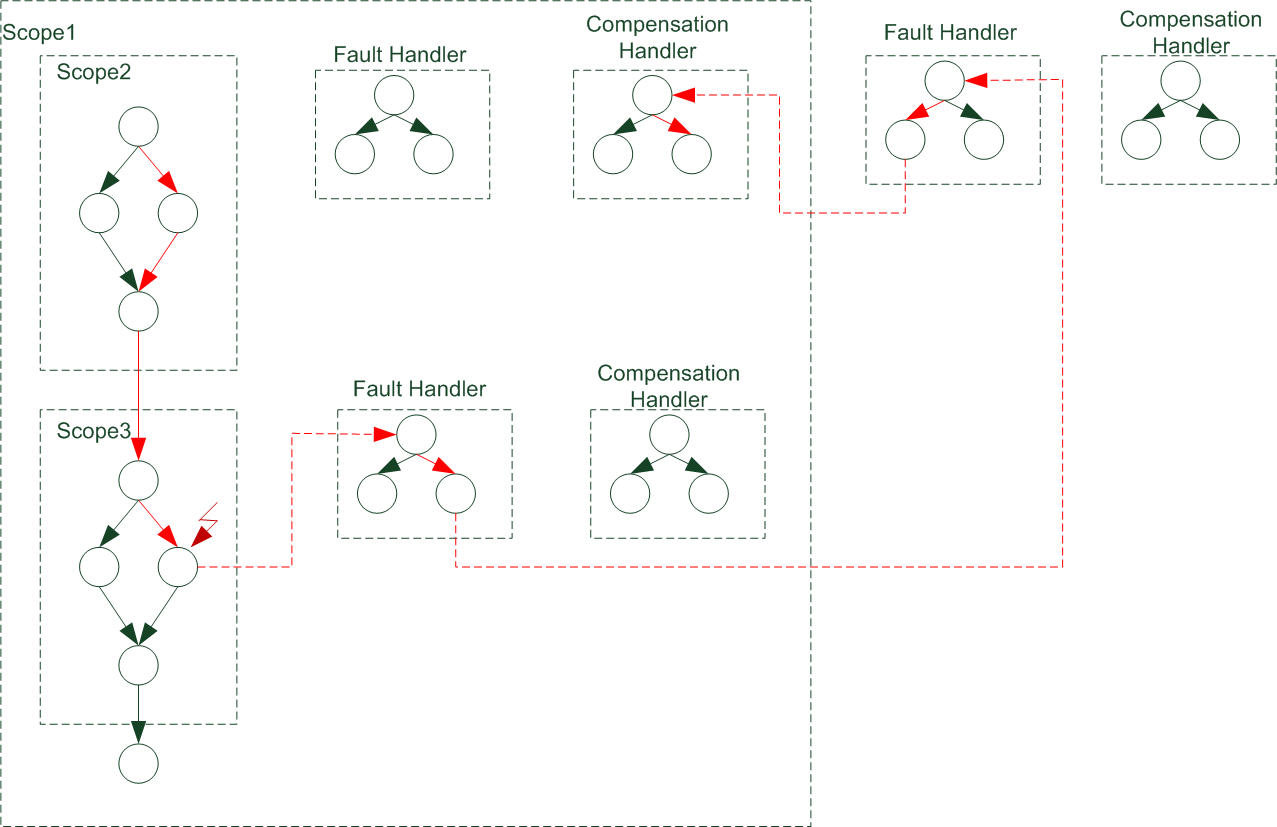
\includegraphics[width=0.9\textwidth]{bilder/Fault_Compensation.png}
		\caption{Kontrollfluss eines BPEL Prozesses}
	\label{fig:ExamlpleBPELProzess}
\end{figure}

Obwohl die Fehlererkennungsquote gegen�ber der Anweisungsabdeckung steigt, werden nicht alle Aspekte des Kontrollflusses erfasst. W�hrend jeder Zweig f�r sich alleine betrachtet wird, bleiben die Kombinationen von Zweigen unber�cksichtigt. 

In den n�chsten beiden Abschnitten werden die f�r WS-BPEL spezifischen
Testabdeckungsmetriken vorgestellt: Link- und Handlerabdeckung.      

\subsection{Link Abdeckung}
Das Link-Konzept ist in WS-BPEL ein wichtiges aber komplexes Modellierungsmittel. Die Links dienen der Synchronisation zwischen parallelen Aktivit�ten. Das Verhalten der Links kann mit Hilfe von \textit{transition} und \textbf{joinCondition} kontrolliert werden. Durch diese Bedingungen ist es m�glich komplexe Logik zu modellieren. Daraus ergibt sich die zwingende Notwendigkeit die Links und deren Verhalten zu testen. 
 
F�r die Definition einer entsprechenden Metrik wird eine Auswertungsfunktion
definiert). Let $f$ be a boolean function (or propositional statement),
$Var(f)$ yields all the propositional variables used in $f$ . Let $F$ be a set
of boolean functions and $B$ be the boolean set (true, false), a variable
assignment of $F$ is a mapping $assign: Var(F)\rightarrow B$, and the set of
all possible variable assignments of $F$ is denoted by $Assign(F)$. An
evaluation function is a mapping $eval: F \times Assign(F)\rightarrow B$
(\cite{Ouyang2005}).

F�r die Tests sind nur die Links relevant, deren transition condition nicht mit
einem konstanten Wert belegt sind, sondern mit einem Ausdruck, der erst zur
Laufzeit ausgewertet werden kann. Es ist dabei wichtig, dass der Ausdruck
sowohl zu $true$ als auch zu $false$ ausgewertet wird, um das Verhalten in beiden F�llen zu testen.

Die entsprechende Metrik hei�t $Link\ Coverage$ und wird wie folgt definiert:
\begin{itemize}
	\item $l \in_{\pi 2}\mathcal{LR}$,
	\item $f=transcon(l)$,
	\item $Assign_{test}\subseteq Assign(f)$ die Menge der Kombinationen von Variablenbelegungen, die beim Testen stattgefunden sind,
\end{itemize}
\begin{equation*}
\begin{split}
\mathcal{L}=\frac{\{\left|l\in_{\pi 2}\mathcal{LR}|Var(f)\neq \emptyset\wedge eval(f,Assign_{test}(Var(f))=true)\right|
}{2*\left|\{l\in_{\pi 2}\mathcal{LR}|Var(f)\neq \emptyset \}\right|}+
\\\frac{\{\left|l\in_{\pi 2}\mathcal{LR}|Var(f)\neq \emptyset\wedge eval(f,Assign_{test}(Var(f))=false)\right|\}}{2*\left|\{l\in_{\pi 2}\mathcal{LR}|Var(f)\neq \emptyset \}\right|}
\end{split}
\end{equation*}
	Damit es m�glich ist, die 100\%  Abdeckung dieser Metrik zu erreichen, werden nur die Links ber�cksichtigt, derenn transition condition mindestenns eine Variable enth�lt ($Var(f)\neq \emptyset$).
	
	Au�erdem ist es wichtig, dass nur die Links beachtet werden, deren transition condition beim Testen ausgewertet wurde und nicht durch $DPE$ auf $false$ gesetzt wurde. Anderenfalls k�nnen sehr einfache Tests, die die zugeh�rige Logik nicht testen, sehr schnell 50\% Abdeckung dieser Metrik erreichen. So eine Metrik w�rde dem Verh�ltnis zwischen Abdeckung und Testqualit�t (siehe Abschnitt ) widersprechen.

\subsection{Fault und Compensation Handler Abdeckung}
WS-BPEL Sprache hat ein Konzept zur strukturierten Behandlung von
Laufzeitfehlern. Die Umschaltung von normalen auf \textit{FaultHandler-}Kontrollfluss erfolgt automatisch beim Auftreten eines Fehlers. Was nichts anderes hei�t, als dass der zugeh�rige \textit{FaultHandler} ausgef�hrt wird. Die Fehler k�nnen auch in den \textit{Compensation} und in den \textit{FaultHandler} selbst auftreten. Die Tatsache, dass die
BPEL-Prozesse langlebig sein k�nnen und in unternehmenskritische Bereichen eingesetzt werden, verdeutlicht die Notwendigkeit, das Verhalten des Systems auch im
Fehlerfall umfassend zu testen. Demzufolge sollten die entsprechenden Handler durch die Tests abgedeckt werden. Die in diesem Abschnitt vorgestellten Metriken
k�nnen dabei als Indikator f�r die Testqualit�t bez�glich der Fehlerbehandlung und Kompensation dienen.

\textbf{FaultHandler.} Eine wichtige Information beim Testen des Systems im
Fehlerfall ist, ob alle  $catch$- bzw $catchAll$-Bl�cken durch die Tests
ausgef�hrt werden.   

\begin{itemize}
	\item $A_{catch}=\{a\in \mathcal{A}^{structured}\cup \mathcal{A}^{basic}|(s,f,a)\in \mathcal{HR}\wedge f\in \mathcal{E}_{fault}\wedge s\in \mathcal{A}_{scope}\}$ die Menge der top-level Aktivit�ten in allen $catch$- und $catchAll$-Bl�cken, 
	\item $\left|A_{catch}\right|$ entspricht der Anzahl von catch- und catchall-Bl�cken
	\item $A^{executed}_{catch}=\{a\in A_{catch}|\exists (s,f,a)\in \mathcal{HR}\wedge branch\_executed((s,f,x))=true\}$ die Teilmenge der Aktivit�ten aus $A_{catch}$, die getestet wurden,
\end{itemize}
\[
FH=\frac{\left|A_{catch}\right|}{\left|A^{executed}_{catch}\right|}
\]

Im Rahmen einer Fehlerbehandlung ist es m�glich, die
eigentlich in sich erfolgreichen Aktionen r�ckg�ngig zu machen. Daf�r sind in
WS-BPEL die Compensation Handler vorgesehen.
\textbf{Compensation Handler.}
\begin{itemize}
	\item $A_{compensation}=\{a\in \mathcal{A}^{structured}\cup \mathcal{A}^{basic}|(s,c,a)\in \mathcal{HR}\wedge c\in \mathcal{E}_{compensate}\wedge s\in \mathcal{A}_{scope}\}$ die Menge der top-level Aktivit�ten in allen Compensation Handler
	\item $\left|A_{compensation}\right|$ entspricht der Anzahl der Compensation Handler
	\item $A^{executed}_{compensation}=\{a\in A_{compensation}|\exists (s,c,a)\in \mathcal{HR}\wedge branch\_executed((s,c,a))=true\}$ die Teilmenge der Aktivit�ten aus $A_{compensate}$, die getestet wurden,
\end{itemize}
\[
CH=\frac{\left|A^{executed}_{compensation}\right|}{\left|A_{compensation}\right|}
\]

Da die Gesch�ftsprozesse in der Regel langlebig sind und dar�ber hinaus sensitive
Daten verarbeiten k�nnen, ist eine ausreichende Fehlerbehandlung zwingend notwendig.
Im Rahmen einer Fehlerbehandlung ist oft das Zur�cksetzen vorangegangener �nderungen erw�nscht. Daf�r sind CompensationHandler in BPEL vorgesehen, die das R�ckg�ngig-machen von eigentlich in sich erfolgreichen Aktionen �bernehmen.

Aufgrund dieser besonderen Wichtigkeit der Fehlerbehandlung muss das Verhalten des Systems im Fehlerfall umfassend getestet werden. Die in diesem Abschnitt vorgestellten Metriken k�nnen dabei als Indikator f�r die Testqualit�t bez�glich der Fehlerbehandlung und Kompensation dienen.
 
\textbf{FaultHandler.}
Eine wichtige Information ist zum Beispiel, ob alle durch den Programmierer vogesehen Fehlerbehandlungen in Form von \textit{catch}- bzw \textit{catchAll}-Bl�cken durch die Tests stimuliert werden. 
Die folgende Definition legt die dazugeh�rige Metrik fest: 
\[
	FaultHandlerAbdeckung=\frac{\text{Anzahl der getesten \textit{catch}- und \textit{catchAll}-Bl�cken }}{\text{Anzahl der \textit{catch}- und \textit{catchAll}-Bl�cken}}
\]

Die impliziten \textit{FaultHandler} werden nicht ber�cksichtigt. Die sogenannten \textit{Inline-FaultHandler}, die direkt in die \textit{invok}e-Aktivit�ten integriert sind, m�ssen dagegen in die Berechnung einflie�en.

\textbf{Compensation Handler.}
Diese Metrik gibt den Abdeckungsgrad der \textit{CompensationHandler} an: 
\[
	CompensateHandlerAbdeckung=\frac{\text{Anzahl der getesten \textit{CompensationHandler}}}{\text{Anzahl der \textit{CompensationHandler}}}
\]
Die \textit{Inline-CompensateHandler} werden ebenfalls ber�cksichtigt. \\
\\






\section{Zusammenfassung}
In diesem Abschnitt wurden Konzepte, Technologien und Werkzeuge beschrieben, die f�r diese Arbeit relevant sind. Besonders ausf�hrlich wurde die BPEL-Sprache behandelt, die im Fokus dieser Arbeit steht. Die detaillierte Beschreibung der Konzepten der Sprache dient dem Verst�ndnis der formalen Definition der Metriken (\ref{}) und Umsetzung der Abdeckungsmessung (\ref{}).

ImAbschnitt Design und Implementierung  
\chapter{Verfahren f�r die Messung der Testabdeckung}

In diesem Abschnitt werden einige Ans�tze f�r die Messung der Testabdeckung in BPEL-Prozessen betrachtet und bewertet. Zum Schluss wird eine geeignete L�sung f�r die Integration in BPELUnit-Framework ausgew�hlt.  


Die Verfahren, die in konventionellen Sprachen f�r die Messung der Abdeckung verwendet werden, k�nnen nicht direkt auf BPEL �bertragen werden. Es m�ssen einige BPEL-spezifische Restriktionen beachtet werden:
\begin{itemize}
\item BPEL-Prozesse werden in speziellen Ablaufumgebungen (\textit{BPEL-Engine}) ausgef�hrt.
\item BPEL-Prozesse k�nnen nur mit Web Services (\textit{partner}) kommunizieren.
\item Gesch�ftslogik wird in BPEL-Prozessen durch Aktivit�ten realisiert. 
\end{itemize} 


Es gibt mehrere M�glichkeiten die Informationen �ber Ablauf eines BPEL-Prozesses zu sammeln: 
\begin{itemize} 
	\item \textbf{Instrumentierung}. Der Quellcode wird vor dem Deployen und Ausf�hren modifiziert, indem bestimmte Aktivit�ten hinzugef�gt werden, die die Ausf�hrung der entsprechenden Codebereichen signalisiereb. 
	\item \textbf{Tracing}. Der Ablauf des Programms wird �ber eine Debug-API der Ablaufumgebung  mitverfolgt.
	\item \textbf{Web Service-Mock's}(\cite{Mayer2006}). W�hrend der Ausf�hrung k�nnen aufgerufene Mock-Partner (Web Services, die durch Mock's ersetzt wurden) ihre Interaktionen mit dem BPEL-Prozess protokollieren. 
	\item \textbf{Log-Dateien der BPEL-Ausf�hrungsumgebung}(\cite{Li2005}). Aus den Log-Dateien der Ausf�hrungsumgebung kann Information �ber den Ablauf des BPEL-Prozesses extrahiert werden. 
\end{itemize}

    
Die dritte und vierte M�glichkeit eignen sich f�r die Messung der Abdeckung nicht werden daher an dieser Stelle nur ganz kurz behandelt. Durch eine Erweiterung der Logik von Web Service-Mock's ist es m�glich, die Interaktionen der Mock's mit dem BPEL-Prozess zu protokollieren. Aus dise Weise lassen sich nur Auusagen �ber externes Verhalten des Prozesses (Kommunikation mit anderen Web Services) machen. Die interne Logik und der Kontrollfluss bleiben w�hrend der Laufzeit verborgen. Zur Ermittlung von Metriken fehlen damit die Informationen �ber die Ausf�hrung des Prozesses. Die Log-Dateien der Ablaufumgebungen, wenn diese �berhaupt existieren, sind anbieterabh�ngig und nicht standardisiert, was diese M�glichkeit auch ausschlie�t. 

Der Instrumentierungs- und Tracingansatz sind als Verfahren f�r die Messung der Codeabdeckung aus dem Bereich der konventionellen Programmiersprachen bekannt. Die beiden Ans�tze wurden in der Masterarbeit von P.Dul \cite{Dul2005} im Bezug auf Programmiersprache Java detailliert untersucht und verglichen.
 
\section{Instrumentierungsansatz.}

\begin{wrapfigure}[14]{r}{6cm}
\centering%
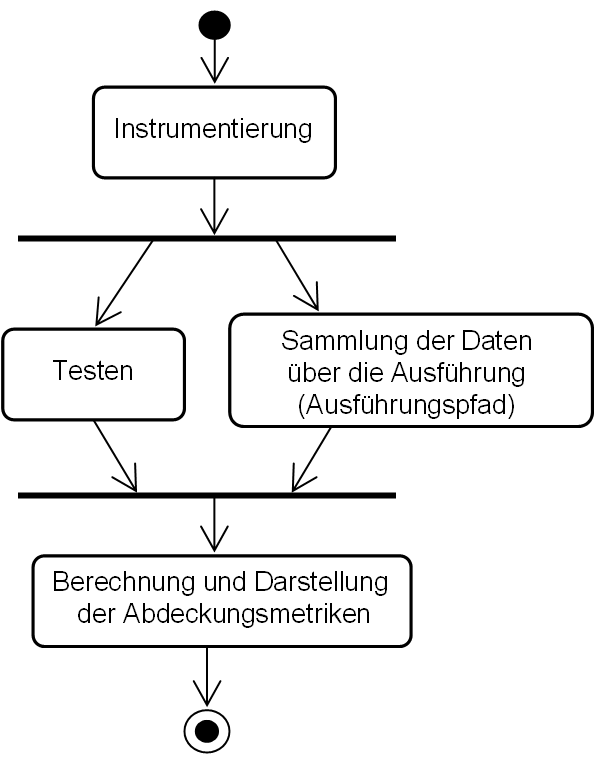
\includegraphics[width=0.3\textwidth]{bilder/Instrumentierung.png}%
\label{}
\end{wrapfigure}
Bei der Instrumentierung handelt es sich um ein einfaches Verfahren zur Messung der Testabdeckung, das in zahlreichen kommerziellen und nicht kommerziellen Werkzeugen eingesetzt wird. 
Dabei werden in den Quellcode zus�tzliche Anweisungen eingef�gt, die die Ausf�hrung bestimmter Codebereiche dokumentieren. Damit der Originalcode unver�ndert bleibt, wird die Instrumentierung auf einer Kopie durchgef�hrt. 

W�hrend der Instrumentierung werden die relevanten statistischen Daten des Quellcodes, die f�r die Auswertung der Ergebnisse notwendig sind, gesammelt und gespeichert. Anhand dieser Daten und der Information, die w�hrend der Ausf�hrung gesammelt wird, kann die Auswertung erfolgen und die Codeabdeckung ermittelt werden. Der Instrumentierungsansatz f�hrt zu einer erheblichen Vergr��erung des Programms.  

Cobertura ist ein bekanntes Werkzeug zur Ermittlung der Testabdeckung in Java-Programmen, das unter General Public License verf�gbar ist und auf dem Instrumentierungsverfahren basiert. 

..........Der Instrumentierungsansatz f�hrt offensichtlich zu einer erheblichen Zunahme der
Programmgr��e: Es wird eine Kopie des originalen Quellcodes generiert. Dann wird
die Kopie instrumentiert

\section{Tracingansatz}
Die modernen Entwicklungsumgebungen verf�gen �ber Debugger, die unter anderem eine Tracing-Funktionalit�t mit sich mitbringen.
\begin{quotation}
	\textit{Tracing bezeichnet man in der Programmierung eine Funktion zur Analyse von Fehlersuche von Programmen.
Dabei wird z.B. bei jedem Einsprung in eine Funktion, sowie bei jedem Verlassen eine Meldung ausgegeben, sodass der Programmierer mitverfolgen kann, wann und von wo welche Funktion aufgerufen wird...Wikipedia}
\end{quotation}
Diese Funktionalit�t erlaubt den Ablauf des Programms zu verfolgen und kann zur Messung der Testabdeckung genutzt werden. Auch bei diesem Ansatz wird der Quellcode im Vorfeld analysiert, um alle relevanten statischen Informationen zu sammeln. 

\section{Vergleich der Verfahren und Auswahl des Ansatzes f�r die Realisierung der Abdeckungsmessung in BPEL}
Die Tabelle \ref{Vergleichstabelle} beruht auf Ergebnissen aus \cite{Dul2005} und stellt die beiden Verfahren im BPEL-Context gegen�ber.
\begin{table}[h!]
\begin{tabular}{p{6cm}p{0.5cm}p{6cm}}
\textbf{Instrumentierungsansatz}&\ &\textbf{Tracingansatz}\\[0.1cm]
\hline \\
Basiert auf dem Hinzuf�gen von
Instrumentierungsanweisungen in
eine Kopie des zu untersuchenden
Quellcodes.&\ &
 Basiert auf den F�higkeiten des
Debuggers, Informationen
�ber das ablaufende
Programm zu erhalten.\\
\\
 Es besteht grunds�tzlich die
Gefahr den Programmablauf oder
die Programmlogik durch das
Hinzuf�gen von Instrumentierungsanweisungen zu
ver�ndern.&\ &
 Es besteht keine Gefahr, dass der
Programmablauf oder die Programmlogik
beim Tracingansatz
ver�ndert werden.\\
\\
 Es besteht grunds�tzlich die
Gefahr von Namenskonflikten
oder der Verletzung der Spezifikation.&\ &
 Es besteht keine Gefahr, dass
Namenskonflikte oder eine
Verletzung der Spezifikation
auftreten.\\
\\
 Overhead wird durch zus�tzliche
Aktivit�ten im Quellcode
generiert.&\ &
 Overhead wird durch die
Anwendung der Debug-API generiert.\\
\\
 Es ist eine aktivit�tsbasierte
Messung der Testabdeckung
m�glich.&\ &
 Es ist nur eine zeilenbasierte
Messung der Testabdeckung
m�glich.\\
\\
Die Messung bleibt unabh�ngig von 
Anbieter der Ablaufumgebung.&\ & 
Die Messung ist nur m�glich, wenn der Anbieter der Ablaufumgebung eine Tracing-Funktion unterst�tzt. Die L�sung ist anbieterspezifisch.
\end{tabular}
\caption{Vergleich der Ans�tze\cite{Dul2005}}
\label{Vergleichstabelle}
\end{table}

Zahlenm��ig weist der Tracingansatz weniger Nachteile auf. Jedoch fehlt es teilweise Unterst�tzung der BPEL-Ablaufumgebungen f�r Debugging bzw. es gibt keine Tracing-Funktionalit�t, die die Verfolgung des Ablaufs erm�glichen w�rde. Noch gr��eres Problem ist, dass diese Schnittstelle in keinster Weise standardisiert ist. Alle Nachteile des Instrumentierungsansatzes entstehen aus der Tatsache, dass die Manipulation des Quellcodes stattfindet. 

Bei der Fallstudie in der oben erw�hnten Masterarbeit wurde festgestellt, dass die Messung beim Tracingansatz wesentlich langsamer ist, als beim Instrumentierungsansatz. Diese Aussage hat aber f�r den BPEL-Prozess, der die Dienste �ber Netzwerk anspricht, keine G�ltigkeit. Der Grund daf�r ist der Netzwerkzugriff, der f�r die Kommunikation notwendig ist. Auch wenn BPELUnit-Framework die M�glichkeit anbietet, den BPEL-Prozess isoliert von den einzelnen Web Servives zu testen, werden die Mock's, die Web Services simulieren, immer noch �ber Netzwerkschicht angesprochen. Die Programmeinheit, die die Meldungen �ber Ausf�hrung bestimmter Codeteile empf�ngt, muss ebenfalls �ber Netzwerkschicht angesprochen werden. Au�erdem muss die Zeit f�r die Instrumentierung ber�cksichtigt werden. Im Kapitel \ref{chap:fallstudie} werden f�r die vorgestellten Beispiele gemessene Zeitdifferenzen angegeben. 


\textbf{Auswahl des Ansatzes f�r die Realisierung der Abdeckungsmessung in BPEL}\ \\
Da nur die ersten beiden Ans�tze (Instrumentierungs- und Tracingansatz) die Realisierung der Abdeckungsmessung f�r alle definierten Abdeckungsmetriken (siehe Abschnitt \ref{metrikdefinition}) im n�tigen Umfang erm�glichen, reduziert sich die Auswahl auf diese Beiden.

Aufgrund der vorgesehenen Integration der L�sung in das BPELUnit Framework muss bei der Auswahl des Verfahrens auf die Kompatibilit�t zum Framework und den darunterliegenden Konzepten geachtet werden.  Eine der zentralen Ziele bei der Konzeption des BPELUnit Frameworks war die Anbieterunabh�ngigkeit. In dieser Hinsicht hat man sich entschieden, den Ansatz \textit{real-life Testen} zu verwenden und damit auf die Verwendung von Debug-API zu verzichten. Das Deployment ist zwar immer noch anbieterspezifisch, die Abh�ngigkeit wurde aber mit dieser Entscheidung auf einen Minimum reduziert. 
Der Einsatz der Tracing-Funktionalit�t f�r die Messung der Testabdeckung w�rde  die Verwendung des Frameworks mit BPEL-Ablaufumgebungen ausschlie�en, die keine Traicing-Funktionalit�t unterst�tzen. Au�erdem m�sste das Framework an jede einzelne \textit{Engine} angepasst werden. Demzufolge eignet sich f�r die Messung der Abdeckung im BPELUnit Framework der Instrumentierungsansatz am Besten. 

\chapter{Umsetzung der Abdeckungsmessung}
In diesem Abschnitt wird die Umsetzung der Abdeckungsmessung f�r BPEL mit dem Instrumentierungsansatz vorgestellt. Die Ermittlung der Testabdeckungsmetriken nach diesem Verfahren erfolgt, wie bereits im Abschnitt \ref{sec:instrumentierungsansatz} erl�utert, im Wesentlichen in drei Phasen:
\begin{itemize}
	\item Instrumentierung (in diesem Fall der BPEL-Datei),
	\item Sammlung der Daten w�hrend der Testausf�hrung,
	\item Auswetung der Daten und Berechnung der Metriken.
\end{itemize}

Die Instrumentierung ist die Kernaufgabe und wird im folgenden Abschnitt ausf�hrlich vorgestellt. Anschlie�end im Abschnitt \ref{sec:auswertung} werden die zwei anderen Phasen erl�utert.  
\section{Instrumentierung des BPEL-Prozesses}\label{sec:umsetzungInstr}
Instrumentierung erfolgt in zwei Schritten. Zuerst wird die BPEL-Dateis mit speziellen Marken annotiert. Jede Marke repr�sentiert dabei ein f�r die jeweilige Metrik relevantes Element und wird in Form eines Kommentars in den Kontrollfluss eingebettet. Im zweiten Schritt wird daf�r gesorgt, dass diese Marken, sobald der Kontrollfluss sie bei der Ausf�hrung erreicht, an spezielle Komponente �bertragen werden, die die empfangenen Daten anschlie�end f�r die Berechnung der Metriken verwendet.

F�r die korrekte Ermittlung der Testabdeckung ist die richtige Platzierung der Marken entscheidend. Dieses Problem kann im ersten Schritt behandelt werden, ohne BPEL-spezifischen Aspekte der Kommunikation ber�cksichtigen zu m�ssen, die erst im zweiten Schritt zum Tragen kommen.
\subsection{Annotation des Prozesses}
Bei der Instrumentierung einer BPEL-Datei sind mehreren Aufgaben zu erledigen:
\begin{itemize}
\item Analyse der BPEL-Datei,
\item Sammlung und Speicherung der statischen Daten (f�r die sp�tere Auswertung),
\item Annotation des BPEL-Prozesses mit Marken.
\end{itemize}
Die Ausf�hrung der Aufgaben erfolgt in drei Phasen, die sequentiell abgearbeitet werden. 

\textbf{Phase 1.} W�hrend der ersten Phase wird der BPEL-Prozess analysiert. Dabei werden f�r jede Metrik alle f�r sie relevanten Elemente des Prozesse bestimmt und gespeichert. Dadurch wird gesichert, dass die Elemente, die w�hrend der Instrumentierung in den Prozess eingef�gt werden, bei der Besimmung der Metriken unber�cksichtigt bleiben. Die relevanten Elemente k�nnen anhand der Definitionen der jeweiligen Metrik (siehe Abschnitt \ref{sec:metrikdefinition}) bestimmt werden:
\begin{itemize}
	\item Aktivit�tabdeckung - alle Basisaktivit�ten,
	\item Zweigabdeckung - alle Strukturierten Aktivit�ten,
	\item Linkabdeckung - alle Links mit \textit{transition condition}, die nicht kostant \textit{true} oder \textit{false} ist,
	\item Fault Handler-Abdeckung - alle \textit{catch}- und \textit{catchAll}-Elemente,
	\item Compensation Handler-Abdeckung - alle Compensation Handler. 
\end{itemize}

\textbf{Phase 2.} Die zweite Phase wird ausf�hrlich in den folgenden vier Abschnitten f�r jede Metrik einzeln vorgestellt. An dieser Stelle werden lediglich einige Bemerkungen gemacht, die f�r jede Metrik gelten. 

In Phase 2 erfolgt die Annotation des Prozesses mit speziellen Marken. Jede Marke ist eindeutig identifizierbar und geh�rt zu einer bestimmten Metrik. Au�erdem identifiziert jede Marke ein Element des Kontrollflusses, das f�r die Abdeckungsmessung relevant ist. Liegen die Marken w�hrend des Tests auf dem Ausf�hrungspfad, so werden diese an eine Komponente �bertragen. Damit protokolliert jede Marke Stimulation eines bestimmten Kontrollflusselements. 
Alle eingef�gten Marken werden gespeichert und stehen f�r die Auswertung und Berechnung der Metriken zur Verf�gung. Bei der Instrumentierung ist zu beachten, dass es grunds�tzlich m�glich ist, die interne Programmlogik des Prozesses  durch die Manipulation zu ver�ndern. Die syntaktische Korrektheit darf nat�rlich auch nicht beeintr�chtigt werden.

In der zweiten Phase wird die BPEL-Datei soweit vorbereitet, dass in der darauf folgenden Phase 3 jede Marke lediglich durch Aktivit�ten ersetzt werden, die die Marken an speziellen Web Service schicken.

Obwohl die Realisierung der Daten�bertragung erst im zweiten Schritt erfolgt, wird zur Vereinfachung bereits in diesem Abschnitt statt einer Marke auch von \textit{Logging} oder \textit{Logging-Aktivit�t} gesprochen.
Grafisch werden die Marken ebenfalls bereits als \textit{invoke}-Aktivit�ten\footnote{Eigentlich geh�rt zu jeder \textit{invoke}-Aktivit�t eine \textit{assign}-Aktivit�t, die die Marken an eine Variable zuordnet. F�r bessere �bersichtlichkeit werden die zugeh�rigen \textit{assign}-Aktivit�ten aber nicht dargestellt.} dargestellt. 
Die Komponente zum Empfangen von Marken wird \textit{Coverage Logging Service} genannt. 

Zu erw�hnen ist noch, dass die Metriken in beliebigen Reihenfolge abgearbeitet werden k�nnen, weil alle ben�tigten Elemente des Originalprozesses f�r alle Metriken in der ersten Phase gespeichert wurden. 


\textbf{Phase 3.} In dieser Phase werden BPEL-Aktivit�ten in den Prozess eingef�gt, die daf�r sorgen, dass die Marken, die beim Testen auf dem Ausf�hrungspfad liegen, an den Web Service �bertragen werden. Dank Vorbereitungen, die in der zweiten Phase gemacht wurden, k�nnen die Marken einfach durch entsprechende Aktivit�ten ersetzt werden, ohne dabei auf die Semantik und Syntax des Prozesses zu achten. 

 
  \subsubsection{Aktivit�tabdeckung}
  Zu betonen ist, dass es  bei der Messung der Testabdeckung nicht darum geht, ob die Aktivit�t \textit{erfolgreich} ausgef�hrt wurde, sondern lediglich darum, ob es zur Ausf�hrung der Aktivit�t kommt. Die Logging-Aktivit�ten, die die Ausf�hrung der Basisaktivit�ten signalisieren sollen, werden im Kontrollfluss direkt vor der jeweiligen Aktivit�t platziert. Bei der \textit{receive}-Aktivit�t kann die Protokollierung ausnahmsweise erst nach der Ausf�hrung stattfinden. Die \textit{receive}-Aktivit�t wird erst ausgef�hrt, wenn sie die Kontrolle hat und eine Nachricht von au�en ankommt. Bei diesem Verhalten darf die Ausf�hrung der Aktivit�t erst nach dem Eintreffen einer Nachricht registriert werden. 
  
  Befindet sich eine Basisaktivit�t in einer \textit{sequence}, so kann die zugeh�rige Logging-Aktivit�t direkt davor oder danach eingef�gt werden. Die Semantik der \textit{sequence}-Aktivit�t sorgt daf�r, dass die Logging-Aktivit�t und die Basisaktivit�t im Kontrollfluss direkt hintereinander erreicht werden. Ist eine Basisaktivit�t in einer anderen Strukturierten Aktivit�t eingebettet, so wird eine \textit{sequence} eingef�gt, die diese Basisaktivit�t und die zugeh�rige Loggingaktivit�t umschlie�t. Durch das Schachtelungsprinzip der Strukturierten Aktivit�ten ist diese Vorgehensweise an jeder Stelle des Prozesses m�glich.
  
  Das Link-Konzept, wie bereits angek�ndigt, braucht eine  besondere Betrachtung. 
  Innerhalb der \textit{flow}-Aktivit�ten erm�glicht das Link-Konzept die Syn\-chro\-ni\-sa\-tions\-ab\-h�n\-gig\-keit\-en zwischen den Aktivit�ten zu definieren und durch die darauf aufbauenden Bedingungen die Ausf�hrung der Aktivit�ten zu steuern (Abschnitt \ref{sec:linkkonzept}). Befindet sich eine eingef�gte Logging-Aktivit�t im Kontrollfluss direkt vor oder nach der Basisaktivit�t, so besteht die Gefahr, dass die Ausf�hrung falsch erfasst wird:
\begin{itemize}
	\item Protokollierung findet vor der Basisaktivit�t statt und die Aktivit�t  selbst wird aufgrund der \textit{transition} oder \textit{join condition} nicht ausgef�hrt.
	\item Protokollierung findet nach der Basisaktivit�t statt, die Aktivit�t selbst wird aufgrund der \textit{transition} oder \textit{join condition} nicht ausgef�hrt und das Attribut \textit{suppress join} ist mit dem Wert \textit{"`yes"'} belegt.
\end{itemize}
In den beiden F�llen wird die Ausf�hrung einer Aktivit�t registriert, obwohl die Aktivit�t gar nicht ausgef�hrt wurde.

Um zu erreichen, dass die Aktivit�t und das Logging entweder beide ausgef�hrt oder beide nicht ausgef�hrt werden, muss die Synchronisation und damit der Link sich auf beide beziehen. Zu beachten ist, dass ein Link genau eine \textit{target}- und eine \textit{source}-Aktivit�t verbinden kann. Damit ist es nicht m�glich, denselben Link f�r die Aktivit�t selbst und f�r die Protokollierung zu verwenden.  Schlie�t man die zu protokollierende Aktivit�t und die Logging-Aktivit�t in eine \textit{sequence} ein und definiert diese als Ziel des Links, so ist das gew�nschte Verhalten erreicht, ohne die Gesch�ftslogik des BPEL-Prozesses zu beeinflussen.  Das gilt f�r beide Werte des \textit{suppress join}-Attributes. 
\begin{figure}[htbp]
	\centering
		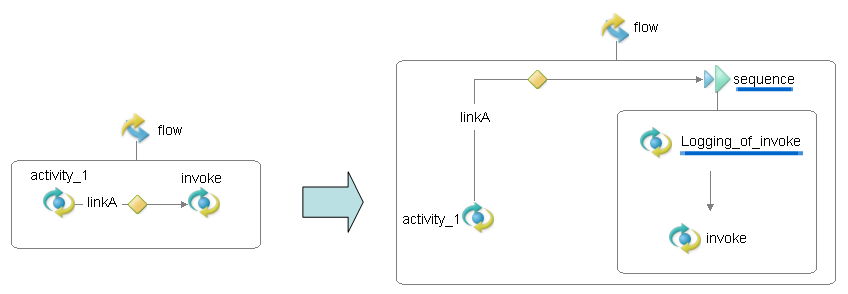
\includegraphics[width=0.83\textwidth]{bilder/ActivityIsTarget.png}
		\caption{Erfassung von Basisaktivit�ten in flow-Umgebung}
	\label{fig:activityAsTarget}
\end{figure}
Die Definition und die Quelle des Links (\textit{source}-Aktivit�t) bleiben unver�ndert. Die Abbildung \ref{fig:activityAsTarget} stellt die Manipulation grafisch dar. Die neu eingef�gten Aktivit�ten sind unterstreichen.

Die entsprechenden �nderungen des XML-Codes:
      %\begin{lstlisting}[caption=\textit{Invoke}-Aktivit�t als Ziel\\ eines Links,numbers=none,label=Listing1]{Name}
\setlength{\columnsep}{1cm}
\begin{multicols}{2}
\lstset{emph={joinCondition,target }, emphstyle=\color{red}}
 
     \begin{lstlisting}[numbers=none,label=Listing1]{Name}
<flow>

	 ...
  <invoke ... joinCondition=...>
    <target linkName="LinkA"/>
  </invoke>  
  
  
</flow>    
  \end{lstlisting}
\lstset{emph={[2]sequence}, emphstyle=[2]\color{blue}}
      \begin{lstlisting}[numbers=none]{Name}          
<flow>
	 ...
  <sequence joinCondition=...>
    <target linkName="LinkA"/>
    <!--Logging-->
    <invoke .../>
  </sequence>
  ...
</flow>      
\end{lstlisting}
\end{multicols}

\subsubsection{Zweigabdeckung}
Die Strukturierten Aktivit�ten bestimmen in BPEL den Kontrollfluss und spielen damit eine entscheidende Rolle f�r die Ermittlung der Zweigabdeckung. Die Zweige werden n�mlich bei der Analyse der Strukturierten Aktivit�ten des Prozesses identifiziert. Die Protokollierung der Zweigen erfolgt im Wesentlichen nach dem Schema, das f�r die Erfassung der Aktivit�tabdeckung vorgestellt wurde. An den entsprechenden Stellen in der BPEL-Datei werden Marken eingef�gt, die das Aktivieren der entsprechenden Zweigen markieren. Damit die Datei bei diesen Manipulationen syntaktisch g�ltig bleibt, wird ebenfalls, wenn es notwendig ist, 
eine umschlie�ende \textit{sequence}-Aktivit�t eingef�gt. 

Ausf�hrlicher werden einige Strukturierten Aktivit�ten vorgestellt, die im Bezug auf die Zweigabdeckung einige Besonderheiten aufweisen.

\textbf{\textit{If}-Aktivit�t.}
Es muss bei diesem Konstrukt darauf geachtet werden, dass der \textit{else}-Zweig erfasst wird. Ist der Zweig nicht explizit im Quellcode vorhanden, dann muss er hinzugef�gt und wie alle anderen Zweige mit einer Marke annotiert werden.

\textbf{\textit{Flow}-Aktivit�t.}
\begin{wrapfigure}[11]{r}{7,2cm}
\centering%
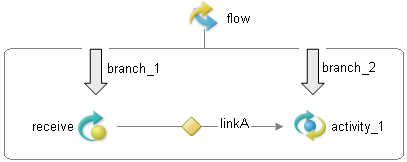
\includegraphics[width=0.45\textwidth]{bilder/FlowCreateInstance.png}%
\caption{Beispiel - Zweigabdeckung in \textit{flow}-Aktivit�t}
\label{fig:zweigabdeckungInFlow}
\end{wrapfigure}
Bei der Messung der Zweigabdeckung in einer \textit{flow}-Aktivit�t m�ssen einige Details beachtet werden. Die Abbildung \ref{fig:zweigabdeckungInFlow} zeigt ein kleines Beispiel, an dem die Problemen und entsprechende L�sung erl�utert werden. Die breiten Pfeile repr�sentieren die Zweige \textit{branch\_1} und \textit{branch\_2}, deren Aktivierung protokolliert werden soll. Jeder BPEL-Prozess muss mindestens eine Aktivit�t enthalten, die die Instanziierung des Prozesses initiieren kann (Attribut \textit{createInstance}=\textit{"'yes"'}). In diesem Beispiel ist das die \textit{receive}-Aktivit�t. Alle anderen Basisaktivit�ten m�ssen im Kontrollfluss hinter dieser Aktivit�t liegen. Der Beispielprozess ist nur aufgrund des Synchronisationslinks \textit{linkA} g�ltig. Der Link sorgt daf�r, dass die \textit{receive}-Aktivit�t vor \textit{activity\_1} abgearbeitet wird. 

F�r die �berwachung dieser Zweige wird der Prozess nach dem bisherigen Schema erweitert. Die Abbildung \ref{fig:ZweigabdReceive} (links) stellt den modifizierten Prozess grafisch dar. Es werden zwei Logging-Aktivit�ten eingef�gt, die jeweils in eine \textit{sequence}-Aktivit�t eingeschlossen sind. Der entstandene Prozess ist nicht mehr g�ltig: die \textit{receive}-Aktivit�t ist nicht mehr die erste Basisaktivit�t im Kontrollfluss.
%\begin{figure}[htbp]
%	\centering
%		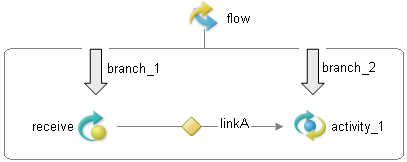
\includegraphics[width=0.5\textwidth]{bilder/FlowCreateInstance.png}
%	\label{fig:createInstanceProblem}
%\end{figure}

 Die Protokollierung der Zweige kann logischerweise erst nach der Erzeugung einer Prozessinstanz erfolgen. Die zugeh�rigen Logging-Aktivit�ten d�rfen im Kontrollfluss nur nach der receive-Aktivit�t platziert werden. Die rechte Abbildung zeigt den Prozess, der diesen Anforderungen entspricht. 
\begin{figure}[htbp]
  \centering
  \begin{minipage}[b]{.485\textwidth}
    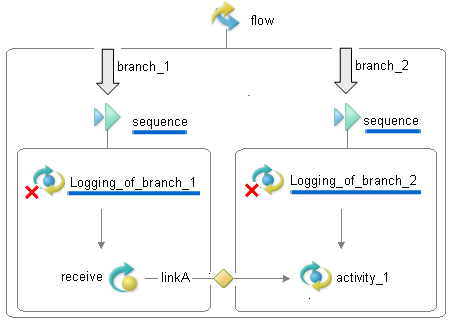
\includegraphics[width=\linewidth]{bilder/FlowCreateInstance2.png}  
  \end{minipage}
  \hspace{0.1cm}
  \begin{minipage}[b]{.485\textwidth}
    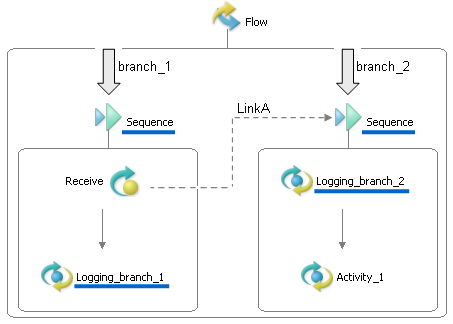
\includegraphics[width=\linewidth]{bilder/FlowCreateInstance3.png}  
  \end{minipage}
      \caption{Erfassung der Zweigabdeckung in einer \textit{flow}-Aktivit�t}
      \label{fig:ZweigabdReceive}
\end{figure}
Die Protokollierung des Zweiges \textit{branch\_1} darf erst nach der Ausf�hrung der \textit{receive}-Aktivit�t stattfinden. Zu Beachten ist, dass die komplette \textit{sequence}-Aktivit�t aufgrund des Links nach der \textit{receive}-Aktivit�t ausgef�hrt wird. Diese Anordnung stellt sicher, dass ein Zweig nur dann als "`abgedeckt"' gilt, wenn die Zielaktivit�t dieses Zweiges zur Ausf�hrung kommt. Es ist sinnvoll, die Aktivierung eines Zweiges im Zusammenhang mit Abdeckungsmetriken wie folgt zu definieren:

\textit{Ein Zweig ist genau dann "`aktiviert"', wenn die Aktivit�t, zu der der Zweig f�hrt, startet bzw. bei \textit{receive}-Aktivit�t wartet auf Nachricht.}

Nur in diesem Sinne "`aktivierte"' Zweige gelten beim Test als abgedeckt.
Das hei�t, dass die Synchronisationslinks ber�cksichtigt werden m�ssen. 
 
%\begin{wrapfigure}[12]{r}{7,5cm}
%\centering%
%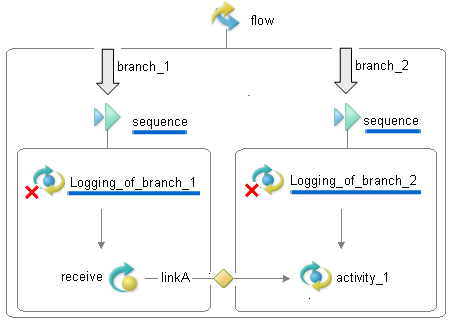
\includegraphics[width=0.48\textwidth]{bilder/FlowCreateInstance2.png}%
%\label{}
%\end{wrapfigure}


 %\begin{figure}[htbp]
	%\centering
	%	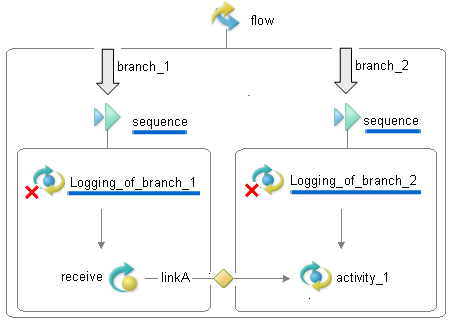
\includegraphics[width=0.5\textwidth]{bilder/FlowCreateInstance2.png}
	%\label{fig:createInstanceProblem}
%\end{figure}
%\begin{wrapfigure}[12]{r}{7,5cm}
%\centering%
%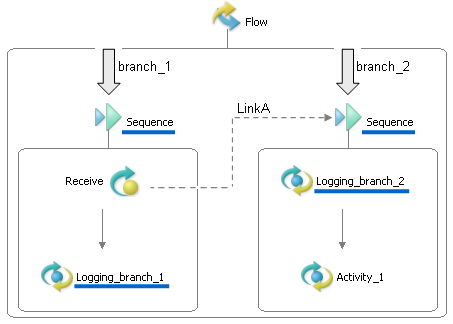
\includegraphics[width=0.48\textwidth]{bilder/FlowCreateInstance3.png}%
%\label{}
%\end{wrapfigure} 
 
 %\begin{figure}[htbp]
%	\centering
%		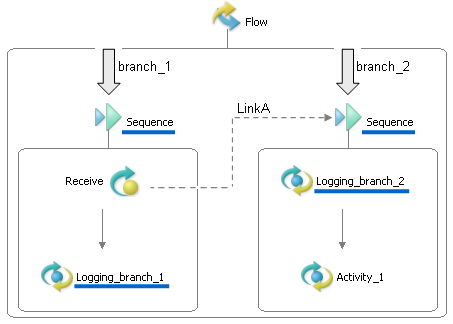
\includegraphics[width=0.5\textwidth]{bilder/FlowCreateInstance3.png}
%	\label{fig:createInstanceProblem}
%\end{figure}
 
 \textbf{\textit{RepeatUntil}-Aktivit�t.}
 Die Auswertung der Bedingung erfolgt bei dieser Wiederholungsschleife erst nach der Ausf�hrung des Schleifenk�rpers. In der Schleife kann man ohne weiteren Logik nicht feststellen, ob das die erste oder bereits wiederholte Ausf�hrung ist. Denn im Falle einer wiederholten Ausf�hrung muss die Aktivierung des Zweiges von der Bedingung zum Schleifenk�rper (in der Abbildung \ref{fig:repeatUntil2} \textit{branch\_2}) signalisiert werden. Die entsprechende �berpr�fung kann mit Hilfe eines Z�hlers, der bei jedem Schleifendurchlauf hochgez�hlt wird, und einer \textit{if}-Abfrage realisiert werden.  Die Z�hlvariable muss nat�rlich im Prozess deklariert und vor der Schleife initialisiert werden. Die entsprechende Modifikation der \textit{repeatUntil}-Aktivit�t ist in der Abbildung dargestellt. Die Deklaration der Variable und die Initialisierung vor der Schleife sind nicht abgebildet.
 \begin{figure}[htbp]
	\centering
		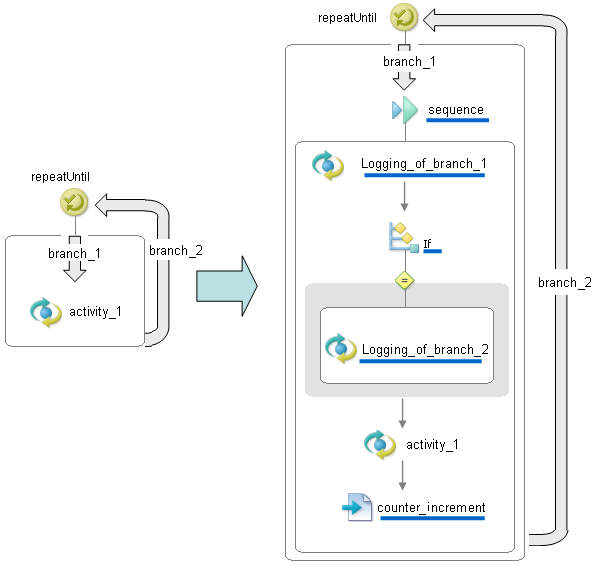
\includegraphics[width=0.65\textwidth]{bilder/repeatUntilZweig.png}
      \caption{Erfassung der Zweigabdeckung in einer \textit{repeatUntil}-Aktivit�t}
	\label{fig:repeatUntil2}
\end{figure}
\FloatBarrier 
\subsubsection{Linkabdeckung}\label{sec:Linkabdeckung}
Es geht bei dieser Metrik um Synchronisationslinks mit einer \textit{transition condition}, die nicht mit einem konstanten Wert \textit{true} oder \textit{false} belegt ist. Die Ermittlung dieser Metrik ist ebenfalls mit Hilfe der Links realisiert. Um die korrekte Erfassung des Linkstatus (\textit{transition condition}) zu erreichen m�ssen folgende Aspekte beachtet werden:
\begin{itemize}
	\item \textit{boundary crossing}-Restriktionen,
	\item unterschiedliche Wertebelegung des \textit{suppress join}-Attributes und daraus resultierendes Verhalten beim Auftreten von \textit{Join Failure},
	\item \textit{Dead-Path-Elimination}.
\end{itemize} 
Diese Aspekte wurden im Abschnitt \ref{restrictions} ausf�hrlich erkl�rt.

\textbf{Beispiel}. Als Grundlage f�r die Erl�uterungen dient folgendes Szenario. Ein Unternehmen  hat einige Strategien entwickelt, um die Gro�kunden trotz gro�er Konkurenz an sich langfristig zu binden. Als besonderen Service wird  zum Beispiel eine bestimmte Lieferdauer f�r diese Kunden  garantiert. Aus diesem Grund ist man  bereit, die Engp�sse auf dem Lager f�r die Gro�kunden durch Bestellungen bei Konkurenz zu �berbr�cken und auf diese Weise kurzfristig sogar Verluste in Kauf zu nehmen. Der Gesch�ftsprozess wird entsprechend der Strategie angepasst und in den IT-Systemen (mit BPEL) umgesetzt. Ein vereinfachter Ausschnitt des zugeh�rigen BPEL-Prozesses ist in der Abbildung \ref{fig:LinkAbdeckungBeispiel} grafisch Dargestellt.
\newpage
\begin{wrapfigure}[12]{r}{7,5cm}
\centering%
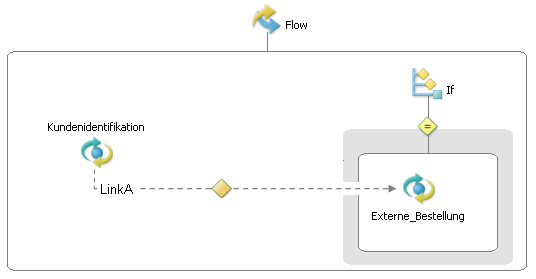
\includegraphics[width=0.48\textwidth]{bilder/FlowBeispiel.png}%
      \caption{Linkabdeckung - Beispielprozess }
\label{fig:LinkAbdeckungBeispiel}
\end{wrapfigure} 
Es gibt zwei Web Services \textit{customer identification}- und \textit{external order}-Service, die von BPEL in dem Prozess aufgerufen werden.   Die daf�r zust�ndigen \textit{invoke}-Aktivit�ten sind in einer \textit{flow}-Umgebung eingebettet. Die \textit{if}-Abfrage (\textit{orderSize}$>$\textit{inventory}) stellt sicher, dass externe Unternehmen nur dann beauftragt werden, wenn die Ware nicht im Lager vorhanden ist. Da die externe Bestellungen nur bei Gro�kunden in Frage kommen, muss erst der Kunde identifiziert werden. Die entsprechende Reihenfolge der Web Service-Aufrufe wird durch das Synchronisationslink \textit{link1} gesichert. Die \textit{transition condition} des Links \textit{customerType='major'} sichert, dass nur die Gro�kunden diesen Service genie�en k�nnen.  


%\begin{figure}[htbp]
%	\centering
%		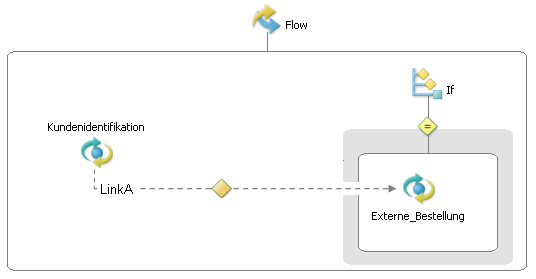
\includegraphics[width=0.5\textwidth]{bilder/FlowBeispiel.png}
%	\label{fig:FlowBeispielDesigner}
%\end{figure}
%\vspace{1cm}

Die Erfassung des Status jedes relevanten Links ist f�r die Ermittlung der Linkabdeckung notwendig. Abh�ngig von dem Wert der \textit{transition condition} muss w�hrend der Ausf�hrung die Marke an den \textit{Coverage Logging Service} verschickt werden, die auf den Wert der \textit{transition condition} zur�ck schlie�en l�sst.  Als m�gliche L�sungen werden drei Ans�tze mit ihren Vor- und Nachteilen vorgestellt und anschlie�end eine ausgew�hlt.

\underline{Variante 1.}\\
Zwei zus�tzliche Links werden definiert (\textit{link1Copy} und \textit{link1Neg}). Dabei �ber\-nimmt der \textit{link1Neg} die negierte  \textit{transition condition} des Originallinks ( \textit{not(customerType='major')}) und  der \textit{link1Copy} die unver�nderte. Die Negierung erfolgt in den meisten Anfragesprachen mit Hilfe der Funktion \textit{not()}. Das gilt sowohl f�r \textit{XPath 1.0} \cite{W3C1999}, die \textit{default}-Sprache in BPEL ist, als auch f�r \textit{XQuery 1.0} \cite{W3C2007a}. Beim Einsatz weiterer Anfragesprachen muss �berpr�ft werden, ob die Funktion \textit{not()} vorhanden ist, und, falls das nicht der Fall ist, muss entsprechende Erweiterungen vorgenommen werden. Die Logging-Aktivit�ten werden bei diesem Ansatz direkt in der \textit{flow}-Umgebung platziert. 
  Dadurch sind sie bereit f�r die Ausf�hrung, sobald der Kontrollfluss die \textit{flow}-Aktivit�t erreicht. Die \textit{source}- und \textit{target}-Aktivit�ten des Originallinks k�nnen dabei beliebig tief in Strukturierte Aktivit�ten eingebettet sein. Durch die am Anfang definierten Links, wird die \textit{source}-Aktivit�t des Originallinks mit den Logging-Aktivit�ten verlinkt. Sobald der Status der Links bekannt ist, wird eine Logging-Aktivit�t ausgef�hrt.

Die \textit{default join condition} der Logging-Aktivit�ten (\textit{or}-Verkn�pfung der Status aller eingehenden Links) und komplement�ren \textit{transition conditions} der beiden neuen Links garantieren, dass nur eine Logging-Aktivit�t gleichzeitig ausgef�hrt werden kann.
%\begin{figure}[htbp]
%	\centering
%		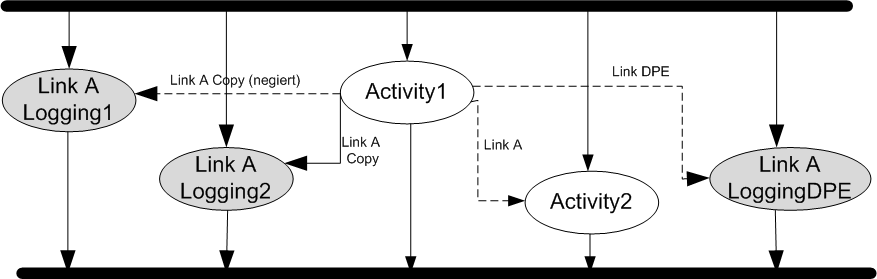
\includegraphics{bilder/LinksAnsatz1.png}
%	\label{fig:LinksAnsatz1}
%\end{figure}
\begin{figure}[htbp]
	\centering
		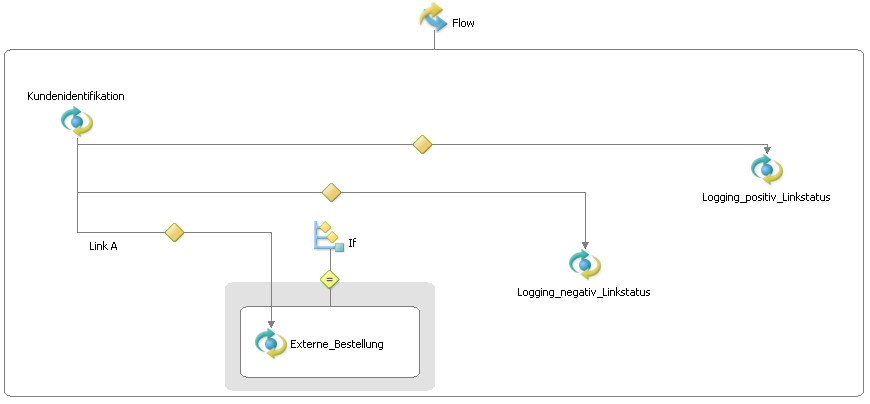
\includegraphics[width=0.98\textwidth]{bilder/FlowBeispielV1.png}
      \caption{Erfassung der Linkabdeckung (erste Variante)}
	\label{fig:LinksAnsatz1Designer}
\end{figure}


\begin{table}[h!]
\begin{tabular}{p{6cm}p{0.5cm}p{6cm}}
\textbf{Vorteile}&\ &\textbf{Nachteile}\\[0.1cm]
\hline \\
Logging kann stattfinden, unabh�ngig davon, ob \textit{external order}-Service aufgerufen wird&\ &\textit{boundary crossing}-Restriktionen k�nnen verletzt werden\\
\end{tabular}
%\caption{Vergleich der Ans�tze}
\label{Vergleichstabelle}
\end{table} 
\FloatBarrier
Die Variante erm�glicht den Linkstatus unabh�ngig von dem Aufruf des Web Services \textit{external order} zu erfassen. Das hei�t, der Linkstatus wird auch dann erfasst, wenn die Bedingung \textit{orderSize}$>$\textit{inventory} zu \textit{false} ausgewertet wird und der Zweig mit \textit{external order}-Service nicht ausgef�hrt wird. Damit wird die formale Definition der Metrik umgesetzt.

Allerdings funktioniert diese Vorgehensweise nicht in allen Situationen. Die Bearbeitung mehrerer Auftr�ge von verschiedenen Kunden kann in BPEL mittels einer Schleife umgesetzt werden. Die \textit{invoke}-Aktivit�t \textit{customer identification} und die komplette \textit{if}-Aktivit�t k�nnen in die Schleife eingebettet werden, um die Bestellungen auf die gleiche Weise nacheinander zu bearbeiten. In dieser Situation w�rde die Instrumentierung der BPEL-Datei nach dem vorgestelltem Verfahren die Syntaxregeln der BPEL-Sprache verletzen: ein Link darf die Grenzen einer Schleife nicht schneiden (\textit{boundary crossing}-Restriktionen, Abschnitt \ref{sec:linkkonzept}).  

\underline{Variante 2.}\\
Ziel dieses Ansatzes ist, die \textit{boundary crossing}-Restriktionen bei der Erfassung der Linkabdeckung einzuhalten. Die Konstruktion der Links \textit{link1Copy} und \textit{link1Neg} erfolgt auf dieselbe Weise.
Bei dieser Variante wird die \textit{target}-Aktivit�t des Links (\textit{invoke}-Aktivit�t \textit{external identification}) mit den beiden Logging-Aktivit�ten in eine \textit{flow}-Aktivit�t eingeschlossen.
%\begin{figure}[htbp]
%	\centering
%		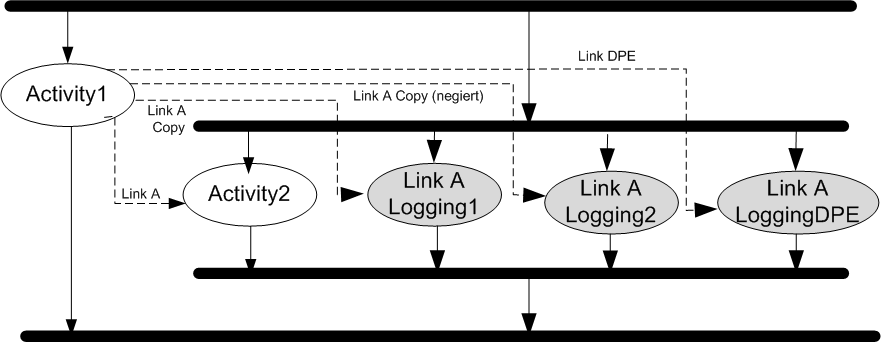
\includegraphics{bilder/LinksAnsatz2.png}
%	\label{fig:LinksAnsatz2}
%\end{figure}
\begin{figure}
	\centering
		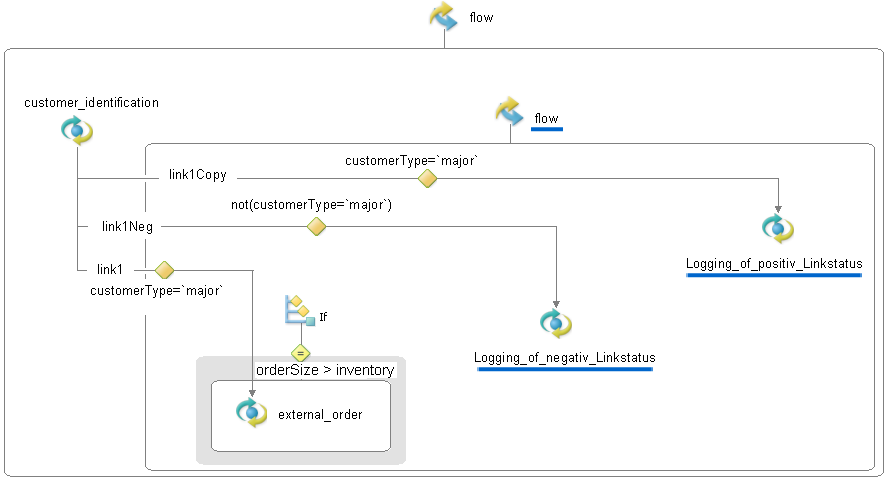
\includegraphics[width=0.95\textwidth]{bilder/FlowBeispielV2.png}
      \caption{Erfassung der Linkabdeckung (zweite Variante)}
	\label{fig:LinksAnsatz2Designer}
\end{figure}


\begin{table}[h!]
\begin{tabular}{p{6cm}p{0.5cm}p{6cm}}
\textbf{Vorteile}&\ &\textbf{Nachteile}\\[0.1cm]
\hline \\
\textit{boundary crossing}-Restriktionen werden eingehalten&\ &Die Links k�nnen nur dann geloggt werden, wenn Web Service \textit{external order} aufgerufen wird.
\\
\end{tabular}
%\caption{Vergleich der Ans�tze}
\label{Vergleichstabelle}
\end{table}
Bei diesem Verfahren schneiden der Originallink und die neu eingef�gten Links dieselben Grenzen der Strukturierten Aktivit�ten.
Setzt man eine syntaktisch g�ltige Ausgangs-BPEL-Datei voraus, so werden keine \textit{boundary crossing}-Restriktionen verletzt. Die eingef�gte \textit{flow}-Aktivit�t kann ebenfalls zu keiner Verletzung f�hren.

Wird die Bedingung \textit{orderSize}$>$\textit{inventory} zu \textit{false} ausgewertet, so k�nnen die Logging-Aktivit�ten nicht ausgef�hrt werden. Der Linkstatus kann in dieser Situation nicht erfasst werden.
\FloatBarrier
\underline{Variante 3.}\\
Bei dieser Variante wird die \textit{source}-Aktivit�t des Links (\textit{customer identification}) mit einer \textit{flow}-Aktivit�t umschlossen. Einerseits sorgt die Platzierung der Logging-Anweisungen in derselben \textit{flow}-Umgebung f�r die Einhaltung der \textit{boundary crossing}-Restriktionen. Andererseits kann das Logging auch stattfinden, wenn die Zielaktivit�t nicht ausgef�hrt wird. Da der Status der Links nach der Ausf�hrung der Quellaktivit�t gesetzt wird, sind die Logging-Aktivit�ten zu diesem Zeitpunkt startbereit und k�nnen gleich die entsprechenden Marken an den \textit{Coverage Logging}-Service verschicken.
%\begin{figure}[htbp]
%	\centering
%		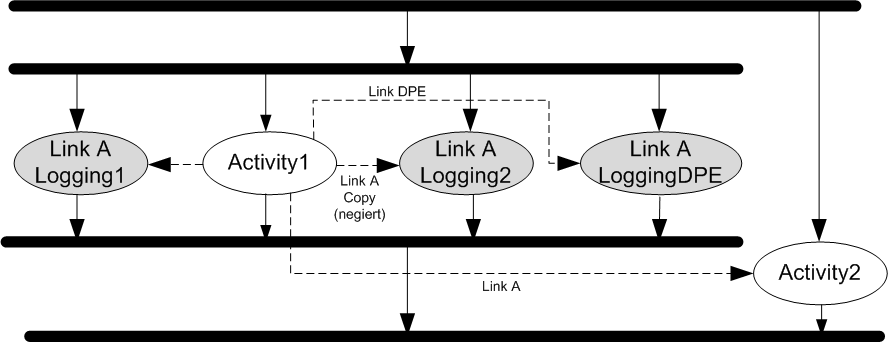
\includegraphics{bilder/LinksAnsatz3.png}
%	\label{fig:LinksAnsatz3}
%\end{figure}
\begin{figure}[htbp]
	\centering
		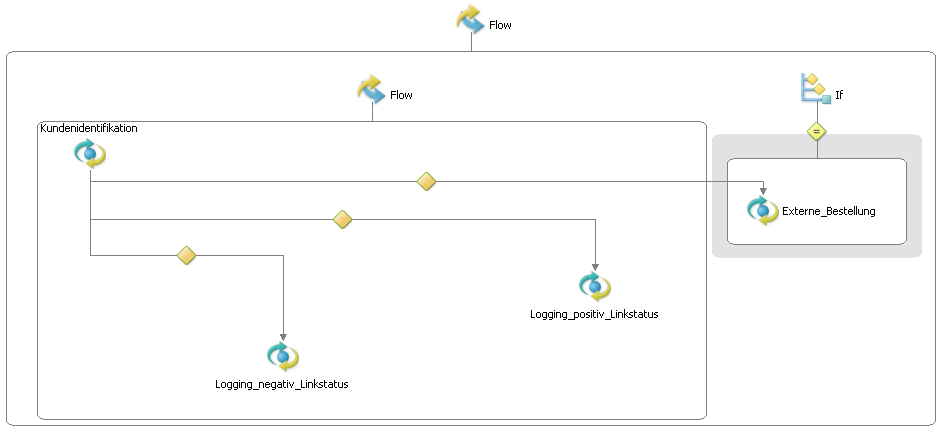
\includegraphics[width=0.95\textwidth]{bilder/FlowBeispielV3.png}
      \caption{Erfassung der Linkabdeckung (dritte Variante)}
	\label{fig:LinksAnsatz3Designer}
\end{figure}

W�hrend die ersten beiden Varianten keine korrekte Messung der Linkabdeckung in allen Situationen erm�glichen, setzt das dritte Verfahren die Definition der Linkabdeckung in allen Situationen ohne Ausnahmen um.
\FloatBarrier
\subsubsection{Fault und Compensation Handler-Abdeckung}
F�r die Fault und Compensation Handler werden die Marken auf dieselbe Weise (mit Hilfe einer umschlie�enden s\textit{equence}-Aktivit�t) in den \textit{catch}- und \textit{catchAll}-Bl�cken bzw. in Compensation Handler platziert. Die folgende Abbildung zeigt entsprechende Modifikationen am Beispiel von Fault Handler.

\begin{figure}[htbp]
	\centering
		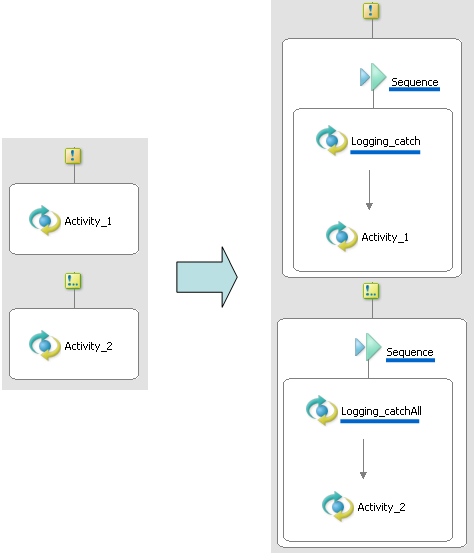
\includegraphics[width=0.65\textwidth]{bilder/FaultHandler.png}
      \caption{Erfassung der \textit{Fault Handler}-Abdeckung}
	\label{fig:LinksAnsatz3Designer}
\end{figure}


Zuvor m�ssen \textit{inline}-Handler (sowohl Fault- als auch Compensation-Handler), die in \textit{invoke}-Aktivit�ten direkt eingebettet sind, umgewandelt werden. Dabei wird die betroffene invoke-Aktivit�t in einen expliziten Scope eingeschlosse, der die Handler auf die �bliche Weise definiert. Die entsprechenden �nderungen des XML-Quellcodes: 

\begin{multicols}{2}
\lstset{emph={invoke}, emphstyle=\color{red}}
      \begin{lstlisting}[numbers=none,label=Listing1]{Name}


<invoke name=...>
    <catch faultName="...">
    ...
    </catch>
    <catchAll>...</catchAll>
    <compensationHandler>
    ....
    </compensationHandler>
</invoke>      
  \end{lstlisting}
\lstset{emph=[2]{scope, faultHandlers}, emphstyle=[2]\color{blue}}
      \begin{lstlisting}[numbers=none]{Name}
      
       
<scope ...>
    <faultHandlers>
        <catch faultName=...>
        ...
        </catch>
        <catchAll>
        ...
        </catchAll>
    </faultHandlers>
    <compensationHandler>
    ...
    </compensationHandler>
    <invoke name=.../>
</scope>     
\end{lstlisting}
\end{multicols}

\FloatBarrier
\subsection{Erweiterung des BPEL-Prozesses f�r die �bertragung der Testabdeckungsdaten}\label{sec:markenuebertragung}
Ein BPEL-Prozess kann nach au�en grunds�tzlich nur mit Web Services kommunizieren. Demzufolge muss der Dienst f�r den Empfang der Nachrichten als Web Service realisiert und w�hrend des Testens erreichbar sein. 
 \begin{figure}[htbp]
	\centering
		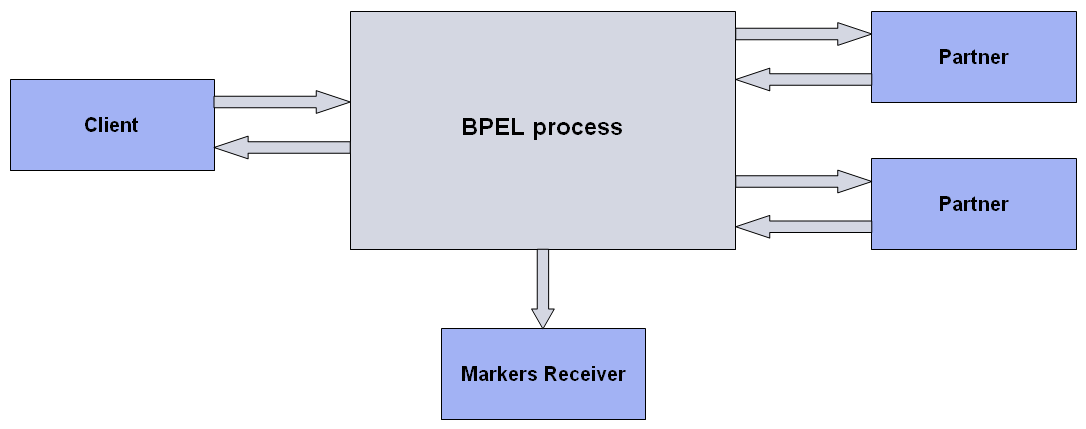
\includegraphics[width=0.75\textwidth]{bilder/bpelProzess.png}
		\caption{Partner eines BPEL-Prozesses}
	\label{fig:loggingservice}
\end{figure}

\textbf{Web Service zum Empfangen von Marken (\textit{Coverage Logging Service})}.

F�r die Kommunikation des BPEL-Prozess mit einem Web Service sind folgende Daten notwendig:
\begin{itemize}
	\item WSDL-Beschreibung,
	\item \textit{Partner Link Type},
	\item \textit{Partner Link}.
\end{itemize}

\underline{WSDL-Beschreibung}. Die einzige Funktionalit�t, die der Service �ffentlich anbieten muss, ist der Empfang von Marken in Form von Zeichenketten. Dementsprechend einfach sieht die Schnittstelle dieses Services aus. Der \textit{Port Type} hat nur eine Funktion \textit{receiveMarkers}, die die Zeichenketten empfangen kann.  Als Nachrichtenprotokoll wird SOAP verwendet. Die Abbildung \ref{fig:webserrvice} zeigt die grafische Darstellung der Schnittstelle.
\begin{figure}[htbp]
	\centering
		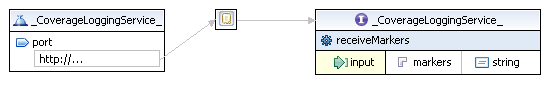
\includegraphics[width=0.7\textwidth]{bilder/WebServiceWSDL.png}
		\caption{WSDL Beschreibung des \textit{Coverage Logging Service}}
	\label{fig:webserrvice}
\end{figure}

\underline{\textit{Partner Link Type}}. Der \textit{Partner Link Type} sowie die WSDL-Beschreibung des \textit{Coverage Logging Services} sind f�r die Kommunikation des BPEL-Prozesses mit dem Service notwendig. Wird der \textit{Partner Link Type} in die WSDL-Datei integriert, was zul�ssig ist, so steht dieser Link in allen BPEL-Dateien, die diese WSDL-Beschreibung referenzieren, zur Verf�gung. Damit entf�llt die Notwendigkeit, den Link explizit zu referenzieren. Aus diesem Grund wird diese L�sung vorgezogen.
\begin{verbatim}
<plnk:partnerLinkType
     xmlns:plnk="http://docs.oasis-open.org/wsbpel/2.0/plnktype"
     name="PLT_CoverageLoggingService_">
   <plnk:role name="MarkersReceiver" 
                     portType="_CoverageLoggingService_" />
</plnk:partnerLinkType>
\end{verbatim}

\underline{\textit{Partner Link}}. \textit{Partner Link} spezifiziert die in \textit{Partner Link Type} festgelegten  Rollen und wird in BPEL-Datei definiert. 
\begin{verbatim}
<partnerLink name="PL_CoverageLoggingService_" 
             partnerLinkType="PLT_CoverageLoggingService_" 
             partnerRole="MarkersReceiver" />
\end{verbatim}

\textbf{Datenaufbereitung und -�bertragen}.
Mit Hilfe von invoke-Aktivit�ten kann ein BPEL-Prozess mit einem Web Service kommunizieren. Die \textit{invoke}-Aktivit�t hat folgende Attributen:
\begin{itemize}
	\item \textbf{partnerLink}: identifiziert \textit{Partner Link}, der f�r die verwendet werden soll,
\item \textbf{portType}:  WSDL-\textit{Port Type} des Zielservices an,
\item \textbf{operation}: WSDL-Operation,
\item \textbf{inputVariable}: Variable, die die zu sendenden Daten enth�lt,
\item \textbf{outputVariable}: Variable, die die Antwort des Services speichert.
\end{itemize}

Soll eine asynchrone Kommunikation realisiert werden oder eine Operation aufgerufen werden, die keine R�ckgabedaten erzeugt, so wird der Attribut \textit{outputVariable} weggelassen. Eine \textit{invoke}-Aktivit�t, die die Marken an den Service verschickt, sieht folgenderma�en aus:  
\begin{verbatim}
<invoke inputVariable="_YXZ_0" 
        operation="receiveMarkers" 
        partnerLink="PL_CoverageLoggingService_" 
        portType="_CoverageLoggingService_" />
\end{verbatim}

Zuvor muss die Variable \textit{\_YXZ\_0} nat�rlich deklariert werden. Damit die Variable im ganzen Prozess benutzt werden kann, wird sie als globale Variable (im \textit{variables}-Element des Prozesses) definiert. Zur Vermeidung der Namenskonflikten werden die Variablennamen aus einem kryptischen Pr�fix und einem Z�hler, der bei jeder Variable hochgez�hlt wird, erzeugt. Da in BPEL durch flow-Aktivit�t die nebenl�ufige Ausf�hrung der Aktivit�ten m�glich ist, muss f�r jeden Zweig eine neue Variable deklariert und als \textit{inputVariable} bei \textit{invoke}-Aufrufen verwendet werden. Die Zuordnung der Marken erfolgt mit Hilfe einer \textit{assign}-Aktivit�t:
\begin{verbatim}
<assign>
   <copy>
      <from>
         <literal>marker1#marker2#markers3</literal>
      </from>
      <to part="markers" variable="_YXZ_0"/>
   </copy>
</assign>
   \end{verbatim}

\section{Auswertung der Daten und Berechnung der Metriken}\label{sec:auswertung}
Beim Instrumentieren des BPEL-Datei werden Marken generiert, die die entsprechenden Aspekte des Kontrollflusses eindeutig identifizieren und zu einer bestimmten Metrik geh�ren. Alle Marken, die in den Kontrollfluss eingef�gt wurden, werden gespeichert und stehen w�hrend und nach der Ausf�hrung des Prozesses zur Verf�gung.
W�hrend der BPEL-Prozess zum Testen ausgef�hrt wird, werden die Marken an den \textit{Coverage Logging}-Service gesendet. 
Die empfangenen Marken liegen auf dem Ausf�hrungspfad und wurden damit durch die Tests abgedeckt. 

Anhand der bei der Instrumentierung gespeicherten und w�hrend der Ausf�hrung gesammelten Daten kann die Testabdeckung ermittelt und Statistiken erstellt werden. Dabei gibt es die M�glichkeit sowohl die Statistik einer ganzen \textit{Testsuite} als auch der einzelnen Testf�llen zu generieren.

\section{Zusammenfassung}
%

Ein BPEL-Prozess kann nach au�en grunds�tzlich nur mit Web Services kommunizieren. Demzufolge muss der Dienst f�r den Empfang der Nachrichten als Web Service realisiert und w�hrend des Testens erreichbar sein. 

 \begin{figure}[htbp]
	\centering
		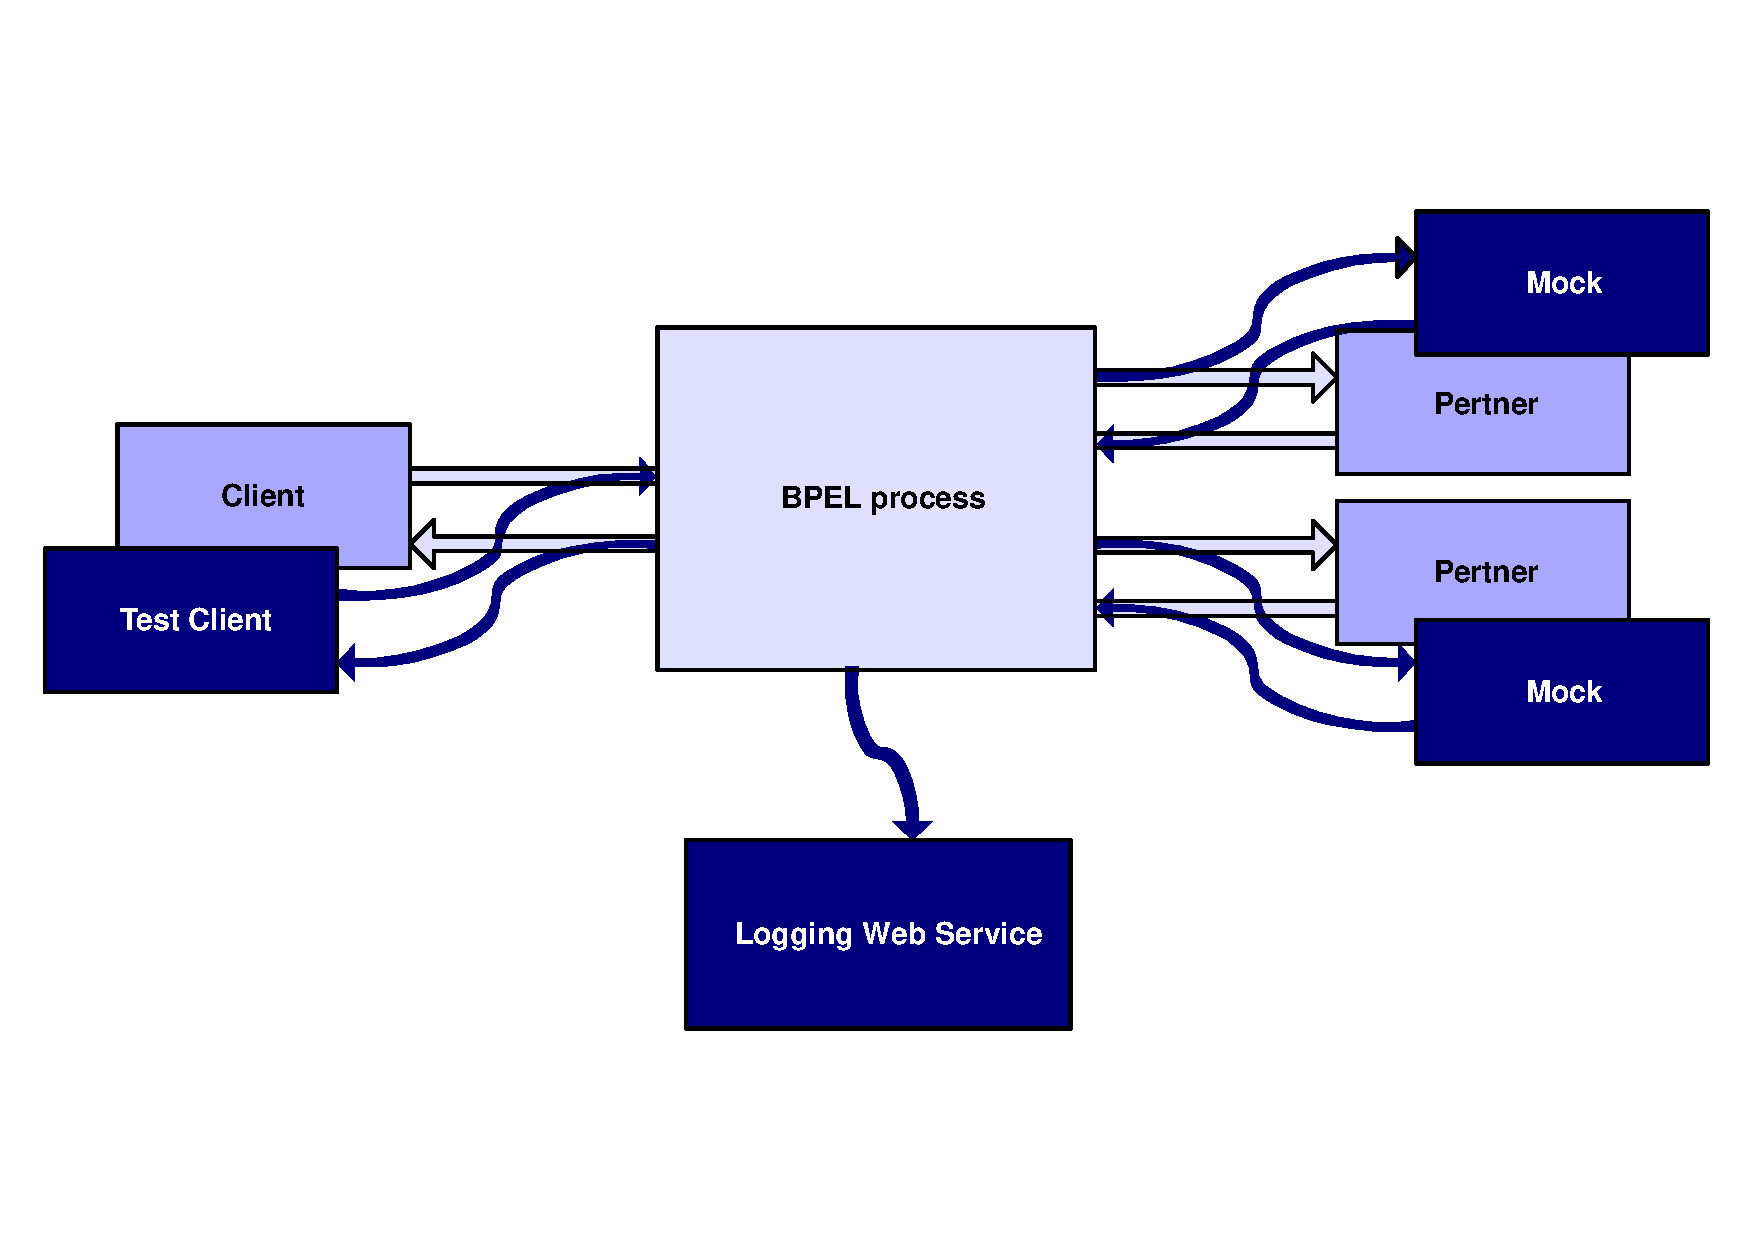
\includegraphics[width=0.90\textwidth]{bilder/loggingservice.pdf}
		\caption{Service}
	\label{fig:loggingservice}
\end{figure}

Die Abbildung \ref{} skizziert den gesamten Ablauf der Abdeckungsmessung.
\begin{itemize}
\item Referenzierung des Web Services im BPEL-Prozess.
\item Annotation des PBPEL-Prozesses durch Marken. Diese Marken sind eindeutig und signalisieren je nach Metrik entweder die Ausf�hrung der Aktivit�ten oder Aktivierung bestimmter Kontrollflusse. Gleichzeitig m�ssen die Daten f�r die sp�tere Auswertung gespeichert werden.
\item Hinzuf�gen von Aktivit�ten, die die Marken an den Service verschicken.		
\item Sammlung der Daten w�hrend der Ausf�hrung des Prozesses.
\item Auswertung der Daten und Ermittlung von Metriken.
\end{itemize} 

Im Abschnitt \ref{sec:empfaengerWS} wird erl�utert, was notwendig ist, damit WS als Kommunikationspartner dem Prozess zur Verf�gung steht. 
Der zweite und der dritte Schritt geh�ren zu der Instrumentierung und werden im Abschnitt \ref{sec:instrumentierung} erl�utert.
Die letzten zwei Schritte werden in Abschnitt erkl�rt.

\section{Referenzierung des Web Services}\label{sec:empfaengerWS}
F�r die Kommunikation des BPEL-Prozess mit dem WS sind f�r den Prozess selbst oder die Engine folgende Daten notwendig:
\begin{itemize}
	\item WSDL Beschreibung
	\item PartnerLinkType
	\item PartnerLink
	\item die konkrete Adresse, unter der der service erreicht werden kann.
\end{itemize}

\textbf{WSDL Beschreibung}. Die einzige Funktionalit�t, die der Service �ffentlich anbieten muss, ist der Empfang von Marken in Form von Strings. Dementsprechend einfach sieht die Schnittstelle dieses Services aus. Der \textit{Port Type} hat nur eine Funktion \textit{receiveMarkers}, die die String empfangen kann. Der Service ist unter einer festen Addresse "`http:\/\/localhost:7777\/ws\/\_CoverageMarkersReceiver\_"' erreichbar.  Die Abbildung \ref{fig:webserrvice} zeigt die grafische Darstellung der Schnittstelle.
\begin{figure}[htbp]
	\centering
		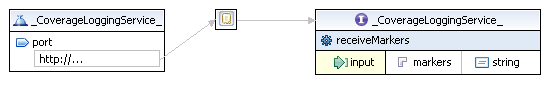
\includegraphics[width=0.7\textwidth]{bilder/WebServiceWSDL.png}
		\caption{WSDL Beschreibung vom Service zum Empfangen von Marken}
	\label{fig:webserrvice}
\end{figure}

\textbf{PartnerlinkType}. Die einfachste M�glichkeit in disem Fall ist, den PartnerLink direkt in der WSDL-Datei zu platzieren.

\begin{verbatim}
<plnk:partnerLinkType
     xmlns:plnk="http://docs.oasis-open.org/wsbpel/2.0/plnktype"
     name="PLT_CoverageMarkersReceiver_">
   <plnk:role name="MarkersReceiver" 
                     portType="_CoverageMarkersReceiver_" />
</plnk:partnerLinkType>
\end{verbatim}

\textbf{PartnerLink}. PartnerLink spezifiziert die in PartnerLinkType festgelegten  Rollen und wird in BPEL-Datei definiert. 
\begin{verbatim}
<partnerLink name="PL_CoverageMarkersReceiver_" 
             partnerLinkType="PLT_CoverageMarkersReceiver_" 
             partnerRole="MarkersReceiver" />
\end{verbatim}


\textbf{Adresse}. F�r den PartnerlinkType m�ssen WSDL service und port sowie konkrette Adresse des Partners festgelegt werden. Diese Information muss der Engine zur Verf�gung stehen und wird in Deployment Descriptor festgelegt. 
\begin{verbatim}
<partnerLink name="PL_CoverageMarkersReceiver_">
  <partnerRole endpointReference="static">
    <wsa:EndpointReference 
    				xmlns:wsa="http://schemas.xmlsoap.org/ws/2003/03/addressing" 
    				xmlns:cov="http://www.bpelunit.org/coverage/CoverageMarkersReceiver">
      <wsa:Address>http://localhost:7777/ws/_CoverageMarkersReceiver_</wsa:Address>
      <wsa:ServiceName PortName="Soap_service_port">cov:_CoverageReportingService_</wsa:ServiceName>
    </wsa:EndpointReference>
  </partnerRole>
</partnerLink>
\end{verbatim}


\section{Instrumentierung}\label{sec:instrumentierung}
Die Instrumentierung eines BPEL-Prozesses besteht aus mehreren Aufgaben:
\begin{itemize}
\item Analyse des BPEL-Prozesses.
\item Sammlung und Speicherung der statischen Daten (f�r die sp�tere Auswertung).
\item Annotation des BPEL Prozesses mit Marken. Jede Marke identifiziert ein relevantes f�r die jeweilige Metrik Aspekt (entweder eine Aktivit�t oder Kontrollfluss�nderung). Erreicht der Kontrollflu� beim Testen die Stelle, an der die Marke positioniert ist, so ist der zugeh�rige Aspekt durch den Test abgedeckt.
\item die Marken von allen Metriken , die im Kontrollflu� unmittelbar hintereinanderliegen, werden zusammengefasst (Optimierung).
\item Hinzuf�gen der BPEL-Aktivit�ten, f�r die �bertragung der Marken an den Web Service f�r Empfang von Marken.	
\end{itemize}
Die Ausf�hrung der Aufgaben erfolgt in drei Phasen, die sequentiell abgearbeitet werden k�nnen. 


\begin{figure}[htbp]
	\centering
		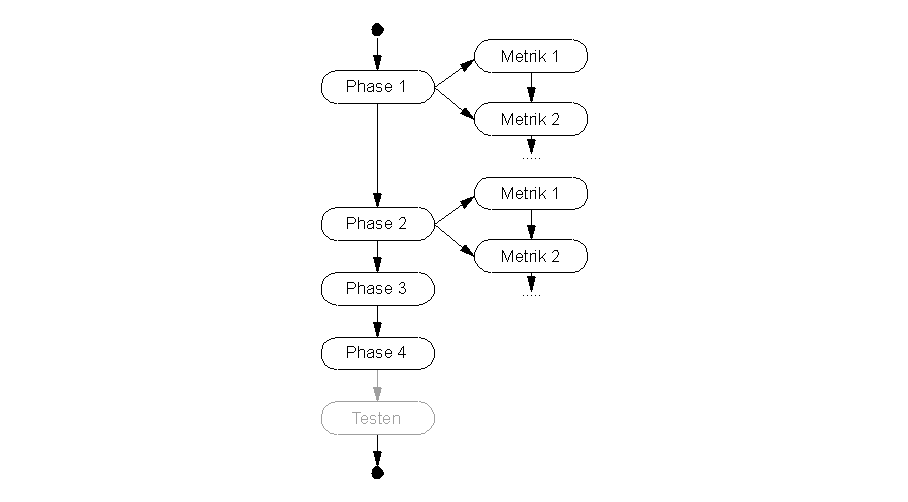
\includegraphics[width=0.5\textwidth]{bilder/Phasen.png}
		\caption{Phasen}
	\label{fig:phasen}
\end{figure}

\textbf{Phase 1.} W�hrend der ersten Phase wird der BPEL-Prozess analysiert. Dabei werden f�r jede Metrik alle f�r sie relevanten Elemente des Prozesse bestimmt und gespeichert. Dadurch wird gesichert, dass die Elemente, die w�hrend der Instrumentierung in den Prozess eingef�gt werden, bei der Besimmung der Metriken unber�cksichtigt bleiben. Die Definitionen der Metriken (siehe Abschnitt \ref{sec:metrikdefinition}) legen die relevanten Elemente des Prozesses f�r die jeweilige Metrik fest:
\begin{itemize}
	\item Aktivit�t Abdeckung - alle Basisaktivit�ten.
	\item Zweigabdeckung - alle strukturierten Aktivit�ten.
	\item Link Abdeckung - alle Links mit \textit{transition condition}, die nicht kostant \textit{true} oder \textit{false} ist.
	\item Fault Handler Abdeckung - alle \textit{catch}- und \textit{catchAll}-Elemente.
	\item Compensation Handler Abdeckung - alle Compensation Handler. 
\end{itemize}

\textbf{Phase 2.} Diese Phase wird ausf�hrlich in den folgenden vier Abschnitten f�r jede Metrik einzeln vorgestellt. An dieser Stelle werden lediglich einige Bemerkungen gemacht, die f�r jede Metrik gelten. 

In dieser Phase werden die statische Daten des Prozesses, die f�r die Ermittlung der Metriken notwendig sind, gesammelt und gespeichert. Gleichzeitig  erfolgt die Annotation des Prozesses mit speziellen Marken. Jede Marke ist eindeutig identifizierbar und geh�rt zu einer bestimmten Metrik. Au�erdem identifiziert jede Marke ein Element des Kontrollflusses, das f�r die Abdeckungsmessung relevant ist.

Die Marken werden, wie bereits erl�utert, in der n�chsten Phase durch invoke-Aktivit�ten ersetzt. Daher bedeutet eine in den Kontrollfluss eingef�gte Marke, dass ein Aspekt des Kontrollflusses an dieser Stelle w�hrend der Ausf�hrung als "`abgedeckt"' markiert wird. Jede Marke repr�sentiert damit die Protokollierung eines Aspekts. Daher wird im weiteren Verlauf der Arbeit bei einer Marke auch von einer \textit{Loggingaktivit�t} oder kurz \textit{Logging} gesprochen. Graphisch werden die Marken ebenfalls als invoke-Aktivit�ten dargestellt. 

F�r die korrekte Ermittlung der Testabdeckung ist die richtige Platzierung der Marken entscheidend. Die entsprechenden Verfahren werden in den folgenden vier Abschnitten f�r jede Metrik einzeln vorgestellt. 

Bei der Instrumentierung ist zu beachten, dass es grunds�tzlich m�glich ist, die interne Programmlogik des Prozesses  durch die Manipulation zu ver�ndern. Die syntaktische Korrektheit darf nat�rlich auch nicht beeintr�chtigt werden. Obwohl die Marken zun�chst als Kommentare eingef�gt werden und damit weder Programmlogik noch die syntaktische Struktur des Programmes �ndern, werden diese Aspekte bereits in dieser Phase beachtet. Der Grund daf�r ist, dass jede Metrik, um bestimmte Aspekte zu erfassen, zus�tzliche Logik braucht (insbesondere im Zusammenhang mit dem Link-Konzept).  Also ist es sinnvoll bereits bei der Platzierung der Marken f�r die semantische und syntaktische Korrektheit des Prozesses zu sorgen, so dass die Marken in der letzten Phase einfach durch entsprechende Aktivit�ten ersetzt werden k�nnen.

Dadurch dass in der ersten Phase alle ben�tigten Elemente des Originalprozesses f�r alle Metriken gespeichert wurden, k�nnen
die Metriken in beliebigen Reihenfolge abgearbeitet werden. 

\textbf{Phase 3.} In dieser Phase werden die Marken, die im Kontrollflu� hintereinander liegen,  zusammengefasst. Anschlie�end werden alle entstandenen Markengruppen  durch BPEL-Aktivit�ten ersetzt, die die Marken an den Web Service verschicken. Die Tatsache, dass der Prozess in der zweiten Phase so aufbereitet wurde, dass die Marken einfach durch Aktivit�ten ersetzt werden k�nnen, vereinfacht diese Phase wesentlich.       


% Ziel: m�glichst wenige Eingriffe in die Logik des Programms.
  Damit die BPEL-Datei syntaktisch korrekt bleibt, muss die Datei f�r die Instrumentierung vorbereitet werden.

  \subsection{Statementabdeckung}

  
  Alle strukturierenden Aktivit�ten (bis auf Sequence) sind so konstruiert, dass sie in ihren Komponenten genau oder maximal eine Aktivit�t erlauben. Durch das Schachtelungsprinzip k�nnen trotzdem beliebig komplexe Strukturen an diesen Stellen eingef�gt werden. Wenn an diesen Stellen nur ein Basic-Aktivit�t vorhanden ist, dann kann man nicht ohne Weiteres dahinter oder davor eine zus�tzliche Aktivit�t hinzuf�gen. Das w�rde zur Verletzung der Syntaxregeln f�hren. Also muss man vor der Instrumentierung eine umschlie�ende strukturierende Aktivit�t hinzuf�gen. Da das Logging entweder direkt davor oder danach statfinden soll, ist die Sequence-Aktivit�t gut f�r diesen Zweck geeignet. 
  
  Innerhalb der Flow-Aktivit�ten erm�glicht das Link-Konzept die Synchronisationsabh�ngigkeiten zwischen den Aktivit�tten zu definieren und durch die darauf aufbauenden Bedingungen die Ausf�hrung der Aktivit�ten zu steuern. Durch das Einf�gen der Protokollieranweisungen alleine kann eine Basic-Aktivit�t, die das Ziel eines oder meheren Links ist, nicht protokolliert werden. ...
  
  L�sung Sequence-Element um diese Aktivit�t und den Link auf die Sequence verschieben. Damit ist die richtige Protokollierung unabh�ngig vom suppressJoin-Wertes garantiert. Die Crossing-Boundary Bedingung wird durch den Eingriff auch nicht verletzt.
  
  
 
\lstset{emph={joinCondition,target }, emphstyle=\color{blue}}
      \begin{lstlisting}[caption=Beispielcode]{Name}
<flow>
  <links>
    <link name="CtoD"/>
  </links>
  <receive name="C" ...>
    <source linkName="CtoD"/>
  </receive>
  <invoke ... joinCondition=...>
    <target linkName="CtoD"/>
  </invoke>
</flow>      \end{lstlisting}

\lstset{emph={[2]sequence}, emphstyle=[2]\color{red}}
      \begin{lstlisting}[caption=Beispielcode][firstnumber=1]{Name}
<flow>
  <links>
    <link name="CtoD"/>
  </links>
  <receive name="C" ...>
    <source linkName="CtoD"/>
  </receive>
  <sequence joinCondition=...>
    <target linkName="CtoD"/>
    <!--Logging-->
    <invoke .../>
    <!--Logging-->
  </sequence>
</flow>      \end{lstlisting}


\subsection{Zweigabdeckung}

Jede Kante wird geloggt durch Einf�gen von Marken vor den Aktivit�ten

otherwise oder else einf�gen

sequenzen Einf�gen

 Flow: beim Fehler.
 
 \subsection{Fault Handler Abdeckung}

\subsection{Compensation Handler Abdeckung}
\chapter{Design und Implementierung}
 
 \begin{figure}[htbp]
	\centering
		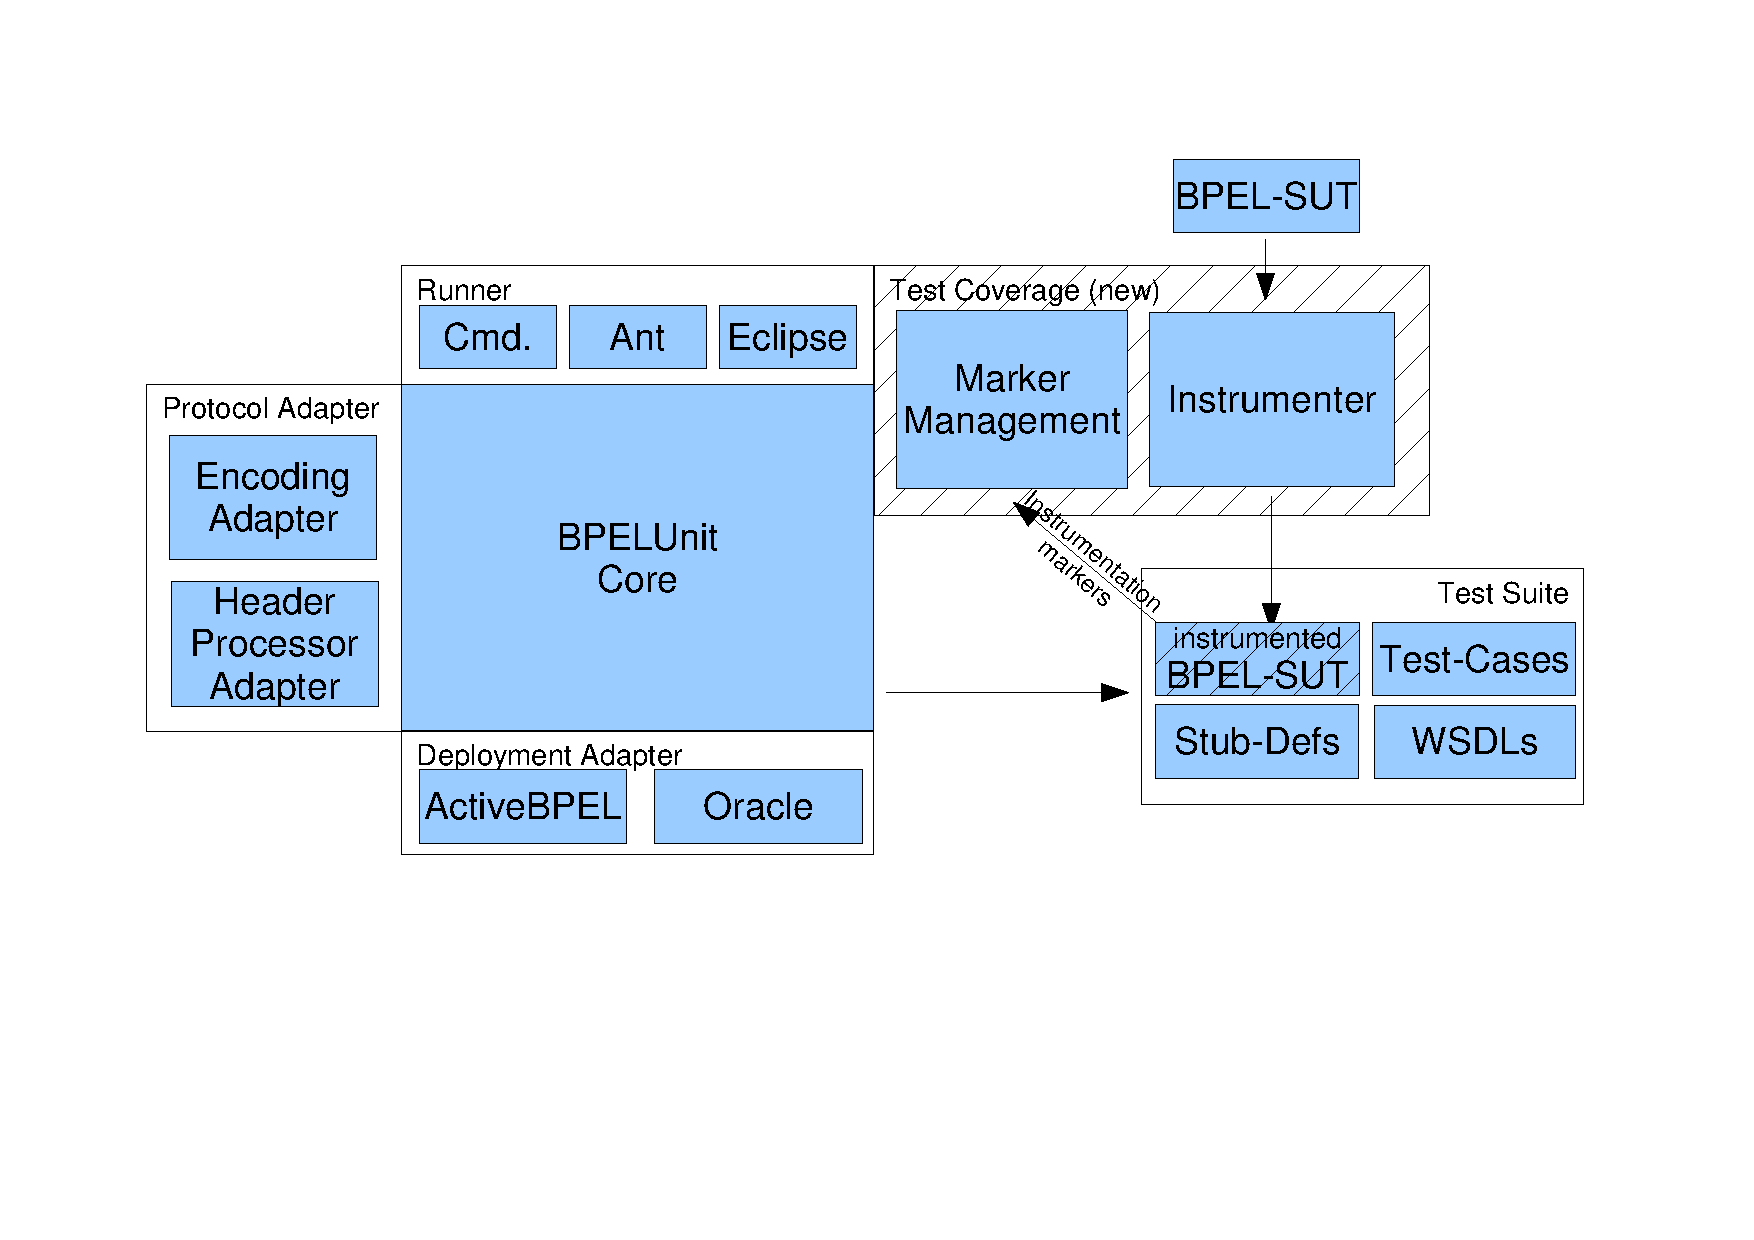
\includegraphics[width=0.9\textwidth]{bilder/bpelunit-architecture-with-coverage.pdf}
		\caption{Kontrollfluss eines BPEL Prozesses}
	\label{fig:ExamlpleBPELProzess}
\end{figure}
\section{Zusammenfassung}
%Ein BPEL-Prozess besteht aus der Gesch�ftslogik (definiert in BPEL), Servicebeschreibung (WSDL) und optional aus weiteren Datentypen (XML Schema). Diese Informationen werden zusammengefasst und in eine BPEL Engine deployt. Die Engine ist unter anderem daf�r verantwortlich, die \textit{Endpoints} der Partner des BPEL Prozesses zu spezifizieren. F�r jeden Link muss bekannt sein, welche WSDL service und port und welche Adresse f�r die Kommunikation benutzt werden sollen. Diese Information wird in so genannten Deployment descriptoren festgelegt.
   Das Deployment und die Syntax der Deploymentdescriptoren ist nicht spezifiziert.



F�r das Testen, wie bereits erl�utert, muss BPEL-Prozess in eine Engine deployt werden. Die BPEL-Dateien mit  den Deploymentinformation werden in einem Archive zusammengefasst und an die BPEL Engine �bergeben. Damit der Web Service f�r den BPEL-Prozess erreichbar ist, muss die WSDL Beschreibung des Web Services in dem Archive enthalten sein. Au�erdem muss f�r die Kommunikation mit diesem Web service ein PartnerLink definiert. F�r diesen Link muss in dem Deployment descriptor die WSDL service und port sowie die konkrete Adresse (in diesem Fall eine feste Adresse auf dem lokalen Host) festgelegt werden.
   Das Deployment und die Syntax der Deploymentdescriptoren ist nicht spezifiziert.

PARTNERLINKTYPE wird in der WSDL Platziert

 Hierzu m�ssen von der jeweiligen BPEL Engine abh�ngige Deployment-Informationen bereitgestellt werden. 

In disem Abschnitt werden zuerst zwei M�glichkeiten f�r die Integration der Messung der Testabdeckung in das Framework vorgestellt. Nach einem Vergleich der beiden Ans�tze wird einen als L�sung ausgew�hlt

Die Aufgabe 

die SOAP-Nachrichten, die an Coverage Receiver gerichtet sind m�ssen dekodiert werden und  an den Servece (Mock) weitergeleitet werden.  

Ansatz1
Es kann ein spezieller Partner Track f�r den Service definiert und zu jedem TestCase zugeordnet werden. Zu jedem Testfall kann dann ein \textit{Thread} gestartet werden, der die Coverage Nachrichten empf�ngt. Es reicht aus jedem TestCase aus. Es muss die Logik f�r den Manager der Marken implementiert werden. Daf�r kann entweder die receive Aktivit�t mehrmals hintereinander geschaltet werden, oder eine neue Aktivit�t, die alle Nachrichten akzeptiert.



 Das Framework dekodiert und leitet weiter , man braucht sich keine Gedanken zu machen. 

nachteil gr��ere Eingriffe in das Framework und an vielen Stellen:
\begin{itemize}
	\item beim Start jedes Testcases muss ein zus�tzliches Thread gestartet werden
	\item beim shutdown unber�cksichtigt 
	\item beim Auswerten des Ergebnissen muss dieser Thread unber�cksichtigt bleiben 
\end{itemize}



Ansatz2

Direkt nachdem Empfangen der Nachricht wird diese an den Receiver weitergeleitet. Dieser muss sich um die Dekodierung der SOAP Nachrichten k�mmern


Dadurch dass beim ersten Ansatz die ganze Funktionalit�t  der Kommunikation (der �bermittlung und Dekodierung der Nachrichten) durch das Framework erledigt werden erscheint diese M�glichkeit als eleganter. Aber Velangsamen
\chapter{Beispiele}\label{beispiele}
In diesem Abschnitt werden die Metriken an einem Besipiel demonstriert. Als Beispiel dient ein sehr einfacher BPEL-Prozess zur Verarbeitung von Bestellungen (Abbildung \ref{fig:Bespielprozess}).
\begin{figure}[htbp]
	\centering
		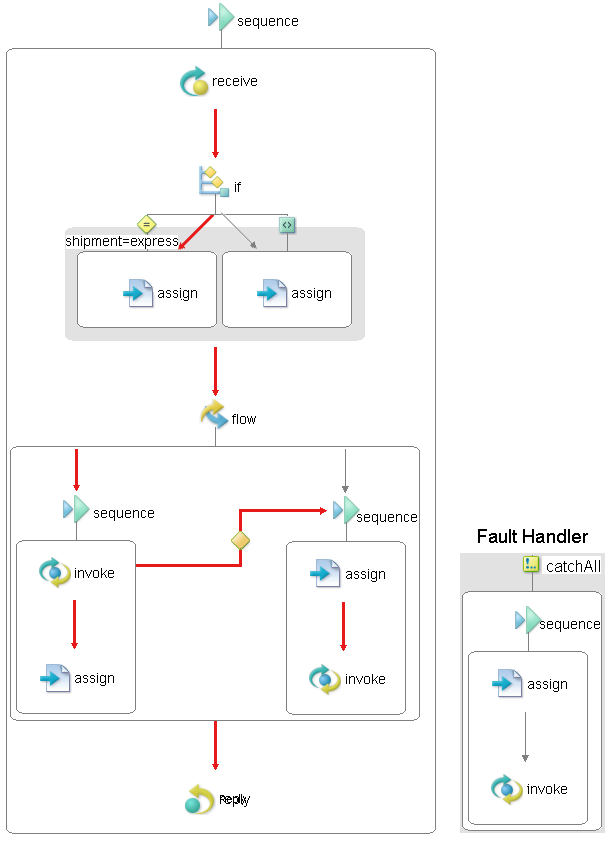
\includegraphics[width=0.6\textwidth]{bilder/Beispiel.png}
		\caption{Beispielprozess}
	\label{fig:Bespielprozess}
\end{figure}

Abh�ngig vom Liefertyp (\textit{express} oder \textit{normal}) werden die Bestellungsdaten unterschiedlich verarbeitet. Wenn der Kunde einen besonderen Status (VIP) hat, was mit dem \textit{Customer Identification}-Service festgestellt wird, dann wir der Kunde und sein Handelsvertreter �ber die Bestellung benachrichtigt.
Das wird mit Hilfe des Synchronisationslinks \textit{link\_1} modelliert, der eine explizite \textit{transition condition} aufweist: \textit{customerType='VIP'}.
F�r den Fehlerfall ist ein einfacher Fault Handler implementiert.

Der Prozess bekommt in einem Testfall eine Bestellung eines \textit{VIP}-Kunden mit folgenden Daten:
\begin{verbatim}
<order>
    <shipment>express</shipment>
    <customerId>12345</customerId>
    <productId>46298</productId>
</order>
\end{verbatim}

Es ist nur wichtig zu wissen, dass der Kunde den VIP-Status hat. Bei der Bearbeitung der Daten wird der mit roten Pfeilen markierte Pfad durchlaufen.
Mit der Erweiterung des BPELUnit-Frameworks kann die Testabdeckung ermittelt werden. Der Befehlszeilen-Client liefert die Testabdeckung im XML-Format:
\begin{verbatim}
<testingCoverage xmlns="http://www.bpelunit.org/schema/coverageResult">
  <FileStatistics filename="bpel/prozess.bpel">
    <statistic name="ActivityCoverage" totalItems="10" testedItems="7" />
    <statistic name="ActivityCoverage: assign" totalItems="5" 
                                                          testedItems="3" />
    <statistic name="ActivityCoverage: invoke" totalItems="3" 
                                                          testedItems="2" />
    <statistic name="ActivityCoverage: receive" totalItems="1" 
                                                          testedItems="1" />
    <statistic name="ActivityCoverage: reply" totalItems="1" 
                                                          testedItems="1" />
    <statistic name="BranchCoverage" totalItems="10" testedItems="8" />
    <statistic name="CompensationHandlerCoverage" totalItems="0" 
                                                          testedItems="0" />
    <statistic name="FaultHandlerCoverage" totalItems="1" testedItems="0" />
    <statistic name="LinkCoverage" totalItems="2" testedItems="1" />
    <statistic name="LinkCoverage: negativLinks" totalItems="1" 
                                                          testedItems="0" />
    <statistic name="LinkCoverage: positivLinks" totalItems="1" 
                                                          testedItems="1" />
  </FileStatistics>
</testingCoverage>
\end{verbatim}


Obwohl es sich um einen sehr einfachen BPEL-Prozess handelt, deckt ein Testfall   bereits 70\% der Basisaktivit�ten und 80\% der Zweige ab. Es wird allerding nur 50\% der Linkabdeckung erreicht und der Fault Handler wird gar nicht getestet. Der Tester kann diese Ergebnisse nutzen, um neue Testf�lle zu definieren und fehlende Bereiche abzudecken.
\chapter{Fallstudie}\label{chap:fallstudie}
Zur �berpr�fung der praktischen Einsetzbarkeit der entwickelten L�sung wurde eine Fallstudie durchgef�hrt. Die Web Service-basierte Anwendung und die zugeh�rigen Tests, die dabei verwendet wurden, sind aus einem studentischen Projekt entstanden: "`Entwicklung einer Web Service-basierten Anwendung"' an der Universit�t Hannover am Fachgebiet Software Engineering (WS 2006/07). 
Innerhalb eines Semesters haben 8 Studenten die Anwendung entworfen, implementiert und getestet. Aufgrund der eingesetzten Technologien und Werkzeuge, wie BPEL (Kompositionsprache), BPELUnit-Framework (Testwerkzeug) und \textit{ActiveBPEL Engine}, hat sich das Projekt als Fallstudie f�r diese Arbeit angeboten. Zu erw�hnen ist noch, dass die BPEL-Sprache noch in der Version 1.1 verwendet wurde.

Entwickelt wurde ein System f�r das Fachgebiet Software Engineering, das den Anmeldeprozess f�r studentische Abschlussarbeiten unterst�tzt. Das System stellt dabei sicher, dass alle wesentlichen Bestandteile der Betreuung, wie z.B. Ver�ffentlichung und Anmeldung der Abschlussarbeit, Planung von Zwischen- und Endvortr�gen, Bewertung usw., eingehalten werden.
F�r die Fallstudie sind vor allem die entstandenen BPEL-Prozesse und die Tests interessant. 

Zur besseren Einsch�tzung der Gr��e der entstandenen Anwendung und Einordnung dieser Fallstudie werden einige statistische Daten des BPEL-Prozesses und (BPELUnit-) Tests vorgestellt.  

Der Gesamtprozess besteht aus 12 Teilprozessen. Insgesamt wurden 13 BPEL-Dateien erstellt: 12 f�r Teilprozesse und eine f�r den Hauptprozess, der alle Teilprozesse (als Web Services) zu einer Anwendung verkn�pft. Die Abbildung \ref{fig:beispielprozess} stellt den Zusammenhang grafisch dar.
Die folgenden Statistiken beziehen sich auf alle 13 BPEL-Dateien und zeigen welche Aktivit�ten bei der Prozessmodellierung verwendet wurden.

\begin{figure}[htbp]
	\centering
		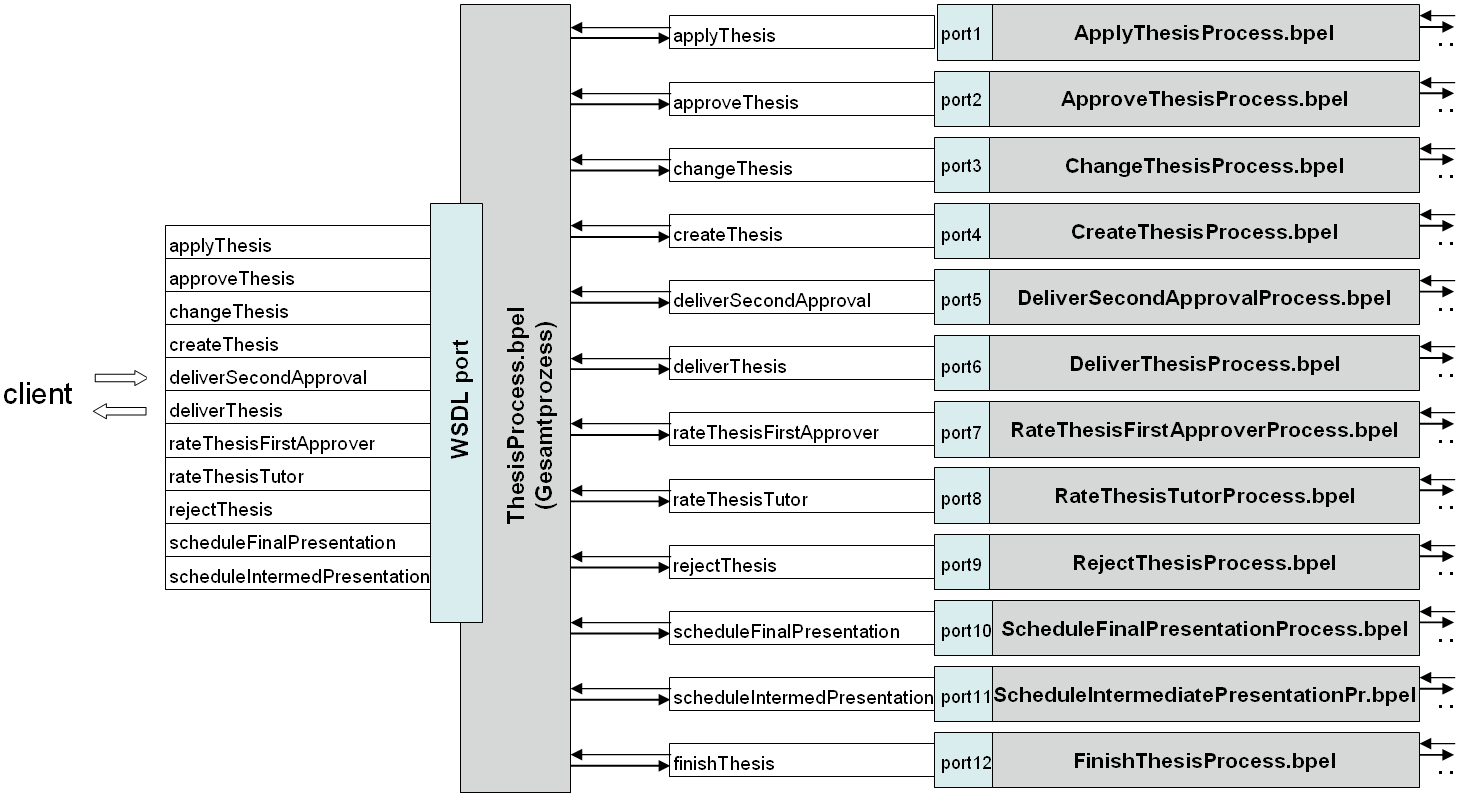
\includegraphics[width=\textwidth]{bilder/Fallstudie.png}
		\caption{BPEL-Prozess. }
	\label{fig:beispielprozess}
\end{figure}

Es wurden insgesamt 508 strukturierten Aktivit�ten und Scopes verwendet:
\begin{table}[h!]
\begin{tabular}{p{2cm}p{0.5cm}p{2cm}}
\textbf{Aktivit�t}&\ &\textbf{Anzahl}\\[0.1cm]
\hline \\
flow&\ &237\\
pick&\ &1\\
switch&\ &71\\
while&\ &19\\
secuence&\ &0\\
scope&\ &180\\
\end{tabular}
\end{table}

\newpage
750 Basisaktivit�ten:
\begin{table}[h!]
\begin{tabular}{p{3cm}p{3cm}p{3cm}p{1cm}}
\textbf{Aktivit�t}&\textbf{Anzahl}&\textbf{Aktivit�t}&\textbf{Anzahl}\\[0.1cm]
\hline \\
assign&387&compensate&0\\
empty&109&invoke&56\\
receive&21&reply&55\\
terminate&14&throw&98\\
wait&10&&\\
\end{tabular}
\end{table}

Auff�llig ist, dass keine \textit{sequence}-Aktivit�ten verwendet wurden;  s�mtliche squentiellen Abl�ufe wurden mit Hilfe von Synchronistaionslinks in \textit{flow}-Aktivit�ten modelliert. Es wurden insgesamt 596 Synchronisationslinks verwendet.

Zum Testen des Prozesses wurde BPELUnit-Framework eingesetzt.
Es wurden zwei Testsuites erstellt:
\begin{itemize}
	\item \textbf{Suite1} besteht aus 30 Testf�llen und testet den gesamten Prozesses. In diesem Fall werden ausschlie�lich die Kommuniaktionspartner (Web Services) der Teilprozesse durch Mocks ersetzt. Die zugeh�rige Aufrufe sind in der Abbildung \ref{fig:beispielprozess} durch kurze Pfeile angedeutet. Das hei�t, es wird ein Prozess getestet, der nicht in einer einzelnen BPEL-Datei beschrieben ist, sondern sich aus mehreren Teilprozessen zusammen setzt. Es werden also nicht die kleinsten Einheiten des Prozesses isoliert.
	\item \textbf{Suite2} besteht aus 12 Testf�llen und testet die einzelnen Teilprozesse. Zus�tzlich zu den Partnern, die bei \textit{suite1} durch Mocks ersetzt wurden, wird auch der Hauptprozess, der in diesem Fall Client ist, durch ein Client-Mock ersetzt.  
\end{itemize}

Die Teilprozesse werden sowohl in \textit{suite1} als auch in \textit{suite2} getestet. Um die gesamte Testabdeckung zu ermitteln, die durch beide Suites zusammen erreicht wird, m�ssen zum einen beide Testsuites ausgef�hrt und zum anderen dieselben Marken verwendet werden, um die abgedeckten Prozesselemente in beiden Testl�ufen identifizieren zu k�nnen. Das BPELUnit-Framework ist allerdings so konzipiert, dass nur eine suite pro Testlauf ausgef�hrt werden kann und die einzelnen Testl�ufe voneinander unabh�ngig sind. 
Die Messung der Testabdeckung erfolgt ebenfalls suite-bezogen. Das hei�t, dass die Berechnung der Testabdeckung �ber mehrere Suites nicht m�glich ist.
F�r die Ermittlung der Testabdeckung mit dem BPELUnit-Framework ist es notwendig, dass alle Testf�lle, die ein Prozess betreffen, in einer Testsuite zusammengef�hrt werden. 

Die Organisation der Testf�lle im betrachteten Projekt erf�llt diese Anforderungen nicht. Aufgrund der unterschiedlichen Schnittstellen, die in den beiden Testsuites f�r die Clients vorgesehen sind, ist auch das Zusammenf�hren der beiden Suites  nicht m�glich. Deswegen kann die Gesamtabdeckung, die beim Testen erreicht wird, nicht ermittelt werden. 
 
 Die praktische Einsetzbarkeit des Verfahrens f�r die Ermittlung der Testabdeckung und die Implementierung k�nnen trotzdem an diesem Projekt �berpr�ft werden. Die Ermittlung der Testabdeckung f�r einzelnen Suites schafft in diesem Fall zwar keine Grundlage f�r die Bewertung der Tests zeigt aber die Funktionst�chtigkeit des entwickelten Werkzeugs an einem realen Projekt.

\textbf{Instrumentierung}. Bei der Instrumentierung werden die BPEL-Dateien (alle 13) f�r alle in dem Abschnitt \ref{sec:metrikdefinition} definierten Metriken instrumentiert. Einige statistischen Daten der Instrumentierungsphase folgen:
\begin{itemize}
	\item 2856 Marken,
	\item 1500 invoke- und assign-Aktivit�ten,
	\item 1094 sequence-Aktivit�ten,
	\item 4 flow-Aktivit�ten.
\end{itemize}

Es werden insgesamt 2856 Marken im Prozess platziert. Die �bertragung der Marken wird durch 1502 \textit{invoke-}Aktivit�ten realisiert. Durch das Zusammenfassen der Marken, die hintereinander im Kontrollfluss liegen, k�nnen 1356 \textit{invoke}-Aktivit�ten gespart werden und damit die \textit{overhead}-Zeit, die durch Ausf�hrung der Aktivit�ten f�r die �bertragung der Marken zustande kommt, verringert werden.  Der getestete BPEL-Prozess enth�lt vier Links, die f�r die Linkabdeckung relevant sind.  Zur Erfassung des Linkstatus wurde f�r jeden Link, wie im Abschnitt \ref{sec:Linkabdeckung} beschrieben, eine \textit{flow}-Aktivit�t eingef�gt.  Die vielen zus�tzlichen \textit{sequence}-Aktivit�ten werden vor allem durch Synchronisationslinks verursacht (siehe Abschnitt \ref{sec:aktivitaetsabdeckung} und \ref{sec:zweigabdeckung}), die im Originalprozess auch f�r die Modellierung der sequenziellen Abl�ufen eingesetzt werden.

\textbf{Ergebnisse}.
Die Ergebnisse sind in der folgenden Tabelle dargestellt.

\textbf{Testsuite1:}
\begin{table}[h!]
\begin{tabular}{p{7cm}p{2cm}p{2cm}p{2cm}}
\textbf{Aktivit�t}&\textbf{Anzahl}&\textbf{Aktivit�t}&\textbf{Anzahl}\\[0.1cm]
\hline \\
Activit�tsabdeckung&750&468&62\%\\
\ \ \ assign&387&277&71\%\\
\ \ \ compensate&0&0&-\\
\ \ \ empty&109&91&83\%\\
\ \ \ invoke&56&56&100\%\\
\ \ \ receive&21&21&100\%\\
\ \ \ reply&55&23&41\%\\
\ \ \ terminate&14&0&0\%\\
\ \ \ throw&98&0&0\%\\
\ \ \ wait&10&0&0\%\\
Zweigabdeckung&1020&704&69\%\\
Linkabdeckung&8&6&75\%\\
\ \ \ negativ&4&3&75\%\\
\ \ \ positiv&4&3&75\%\\
Fault Handler-Abdeckung&64&0&0\%\\
Compensation Handler-Abdeckung&0&0&-\%\\
\end{tabular}
\end{table}
\FloatBarrier
\textbf{Testsuite2:}
\begin{table}[h!]
\begin{tabular}{p{7cm}p{2cm}p{2cm}p{2cm}}
\textbf{Aktivit�t}&\textbf{Anzahl}&\textbf{Aktivit�t}&\textbf{Anzahl}\\[0.1cm]
\hline \\
Activit�tsabdeckung&750&378&50\%\\
\ \ \ assign&387&225&58\%\\
\ \ \ compensate&0&0&-\\
\ \ \ empty&109&85&77\%\\
\ \ \ invoke&56&44&78\%\\
\ \ \ receive&21&12&57\%\\
\ \ \ reply&55&12&21\%\\
\ \ \ terminate&14&0&0\%\\
\ \ \ throw&98&0&0\%\\
\ \ \ wait&10&0&0\%\\
Zweigabdeckung&1020&570&55\%\\
Linkabdeckung&8&2&25\%\\
\ \ \ negativ&4&1&25\%\\
\ \ \ positiv&4&1&25\%\\
Fault Handler-Abdeckung&64&0&0\%\\
Compensation Handler-Abdeckung&0&0&-\%\\
\end{tabular}
\end{table}


\FloatBarrier
Wie bereits erl�utert, kann die Gesamtabdeckung aufgrund der �berschneidungen der Testsuites nicht ermittelt werden. Es fehlt damit die Grundlage f�r die Bewertung der Tests.

\textbf{Zeitmessungen}.
Die Testlaufzeiten werden aufgrund der zus�tzlichen Instrumentierungsphase und neuen Aktivit�ten im Prozess gr��er.
Die gemessenen Zeiten mit und ohne der Ermittlung der Testabdeckung sind in der Tabelle \ref{tab:testlaufzeiten} f�r die beiden Testsuites angegeben (in Sekunden).
Das System auf dem die Testlaufzeiten gemessen wurden hat folgende Charakteristiken:
\begin{itemize}
	\item CPU: AMD Athlon XP 2,17 GHz
	\item Speicher: 2GB
	\item Betriebssystem: Windows XP
\end{itemize}
Die verwendete Software ist im Anhang angegeben \ref{}.

 Nach jedem Testfall wird der Testlauf angehalten, um auf die Coverage-Nachrichten zu warten, die noch �bertragen werden (siehe Abschnitt \ref{sec:coverageLoggingService}). Die Wartezeit kann durch den Tester bestimmt werden. Der optimale f�r diese Fallstudie Wert wurde experimentell ermittelt und betr�gt 0,5 Sekunden.  Die gesamte Wartezeit f�r jede Testsuite ergibt sich aus der Anzahl der Testf�lle und der Wartezeit pro Testfall und ist in der letzten Spalte angegeben. Die Instrumentierungsphase ist f�r die beiden Testsuites gleich und betr�gt 2,2 Sekunden.
 \begin{table}[h!]
\begin{tabular}{p{7cm}p{2cm}p{3cm}}
&\textbf{Laufzeit}&\textbf{Wartezeit}\\[0.1cm]
Testsuite1&\\
\ \ \ \ \ \ \ \ \ ohne Messung der Testabdeckung&$24,3\ s$\\
\ \ \ \ \ \ \ \ \ mit Messung der Testabdeckung&$68,7\ s$&$0,5*30=15\ s$\\
\\
Testsuite2&\\
\ \ \ \ \ \ \ \ \ ohne Messung der Testabdeckung&$14,6\ s$\\
\ \ \ \ \ \ \ \ \ mit Messung der Testabdeckung&$32,8\ s$&$0,5*12=6\ s$\\
\end{tabular}
\caption{Fallstudie - Testlaufzeiten mit und ohne der Ermittlung der Testabdeckung}
\label{tab:testlaufzeiten}
\end{table}

In den Laufzeiten mit der Ermittlung der Testabdeckung ist die Instrumentierungszeit und Wartezeit enthalten.
Die Ausf�hrungszeit hat sich bei der ersten Suite um Faktor 2,8 (ohne Instrumentierungsphase 2,7) und bei der zweiten um Faktor 2,2 (2,1) verl�ngert. Der Faktor  h�ngt sehr stark von dem getesteten Prozess und der Testlogik ab. Aus dem Grund l�sst sich kein Faktor angeben, der allgemein g�ltig ist. 
\chapter{Zusammenfassung und Ausblick}
F�r BPEL-Prozesse, die meistens zu der unternehmenskritischen Software z�hlen, ist die Qualit�t der Tests sehr wichtig. Die Wahrscheinlichkeit, Fehler und M�ngel zu identifizieren, steigt mit zunehmendem Wert des Testabdeckungsma�es.

In dieser Arbeit wurden Codeabdeckungsmetriken f�r BPEL-Prozesse definiert:
\begin{itemize}
	\item Aktivit�tabdeckung: zeigt, wie viele Basisaktivit�ten bei den Tests ausgef�hrt wurden,
	\item Zweigabdeckung: zeigt, wie viele Zweige bei den Tests aktiviert wurde,
	\item Linkabdeckung: zeigt, wie viele Links bei den Tests ausgewertet wurden,
	\item Fault und Compensation Handler-Abdeckung: zeigt, wie viele Handler bei den Tests ausgel�st wurden.
\end{itemize}

Bei der Definition der Metriken wurde darauf geachtet, dass f�r jeden BPEL-Prozess 100\%-ge Abdeckung erreichbar ist. 

Implementiert wurde die Messung der Testabdeckung als Erweiterung des BPELUnit-Frame\-works. Die Instrumentierung der BPEL-Dateien und Ermittlung der Testabdeckung erfolgt automatisch und transparent w�hrend eines Testlaufs. Es kann nur suite-bezogene Testabdeckung ermittelt werden, was keine wirkliche Einschr�nkung darstellt, wenn die Teilprozesse einzeln (jeweils eine BPEL-Datei) isoliert und getestet werden. Es werden zwei Versionen der BPEL-Sprache unterst�tzt: 1.1 und 2.0. Die Erkennung erfolgt automatisch und erfordert keine zus�tzlichen Konfigurationen. Der Eclipse-Plugin und der Befehlszeilen-Client wurden entsprechend erweitert. Die beiden Clients bieten die M�glichkeit die Metriken festzulegen, diese zu konfigurieren und nach dem Testlauf die ermittelte Testabdeckung anzuzeigen.

Der n�chste logische Schritt ist die Visualisierung. Die grafische Darstellung der Testabdeckung kann den Testentwickler bei der gezielten Testerstellung besser unterst�tzen.
F�r das Erreichen der gew�nschten oder geforderter Testabdeckung ist diese Vorgehensweise viel effizienter und kann positive Auswirkungen auf die Entwicklungszeit und -Kosten haben.

Interessant w�re eine Erweiterung des BPELUnit-Frameworks, die die Ausf�hrung mehrerer Testsuites erm�glichen w�rde. Damit w�re es auch m�glich die Testabdeckung �ber mehrere \textit{Suites} zu ermitteln. 

Ein weiterer sehr interessanter Aspekt ist die Unterst�tzung der Anforderungsabdeckung f�r BPEL-Prozesse und die Definition der anforderungsbasierten (\textit{black box}-) Tesdtabdeckungsmetriken.

Die implementierte Erweiterung des BPELUnit-Frameworks bietet eine einfache M�glichkeit, die Komplexit�t des Prozesses zu berechnen. Eine entsprechende Anpassung der Definition von Komplexit�t f�r BPEL wurde in \cite{Cardoso2006} vorgeschlagen.



%
Die prim�re Aufgabe der Code-Coverage-Analyse liegt darin, die im Code durch Tests abgedeckten Bereiche  zu identifizieren und einige Kennzahlen der Abdeckungen zu ermitteln
(z.B. Anzahl der Durchl�ufe einer Codezeile). Daher werden bei der Code-Coverage-Analyse w�hrend der Testausf�hrung
verschiedene Messungen durchgef�hrt, die jeweils Informationen �ber eine bestimmte Art der Abdeckung sammeln. Im
Folgenden werden die wichtigsten Messmetriken bei der Code-Coverage-Analyse aufgelistet.
wieviel des zu untersuchenden Codes tats�chlichdurch die Tests ausgef�hrt wurde. Es wird auch oft der Begriff \textit{Testabdeckung} verwendet.



Anweisungs�uberdeckung wird im allgemeinen nicht als hinreichendes Kriterium
f�ur die Vollst�andigkeit eines Tests betrachtet, ihre Auswertung ergibt sich als
Nebenprodukt der Auswertung umfassenderer �Uberdeckungskriterien. Empirische
Untersuchungen zeigen eine Fehlererkennungsrate von 15\% bis unter 20\% f�ur
reine Anweisungs�uberdeckung. Sie liefert allerdings in allen Untersuchungen h�ohere
Prozents�atze als die statische Analyse des Quelltextes.
Die Kanten�uberdeckung gilt als Standard bei kontrollflussbasierten �Uberdeckungsma�en
und wird oft als Kriterium an Tests gestellt. Sie wird als leistungsf
�ahiger Test vor allem zum Auffinden von logischen Fehlern betrachtet. Untersuchungen
bez�uglich der Leistungsf�ahigkeit streuen in einem weiten Bereich von
20\% bis 70\% gefundener Fehler. Zumeist liegen die Prozents�atze im unteren Drittel
dieses Intervalls. Studien, die ebenfalls Anweisungs�uberdeckung betrachten, zeigen
f�ur Zweig�uberdeckung eine Fehlererkennungsrate, die um 50% bis 100% �uber der
der Anweisungs�uberdeckung liegt.
Bedingungs�uberdeckung findet vor allem bei Systemen mit komplexer Verarbeitungslogik
Verwendung, die in der Regel kompliziert aufgebaute Bedingungen
verwende.



D

Erfolgsquote:
..Anweisungs�berdeckungstest 18%
..Zeig�berdeckungstest 32%
..Bedingungs�berdeckungstest ?
..Pfad�berdeckungstest 65%


Beim Erstellen von Tracedaten unterscheidet man zwischen Methoden, die es erfordern
den bestehenden Source- bzw. Objektcode zu instrumentieren und Methoden,
die automatisch Traceausgaben erzeugen. Moderne Entwicklungsumgebungen bieten
meist Techniken an, um Traceausgaben ohne Sourcecode-�Anderung zu erstellen.


Die Testabdeckungsanalyse gibt an, in welchem Umfang die durchgef�hrten Tests die zu testende Software erfasst haben.



Bis jetzt wurde Instrumentierungsansatz allgemein betrachtet, ohne auf eine bestimmte Sprache einzugehen. Jetzt werden BPEL-spezifische Einschr�nkungen untersucht. Als Erstes d�rfen nur BPEL-Aktivit�ten eingef�gt werden, sonst kann der BPEL-Prozess von der BPEL-Engine nicht ausgef�hrt werden. Um Protokollierung zu realisieren, muss eine Kommunikation von der Ausf�hrungsumgebung nach au�en stattfinden. Die einzige daf�r geeignete Aktivit�t ist \textit{invoke}. Au�erdem muss ein (lokales) Web Service eingerichtet werden, der f�r das Protokollieren zust�ndig ist. Bevor zu tief in die Details eingestiegen wird, werden zuerst die anderen L�sungsm�glichkeiten vorgestellt und besprochen.	
	
	
	\begin{itemize}
\item BPEL-Prozesse werden in speziellen Ablaufumgebungen (\textit{BPEL-Engine}) ausgef�hrt.
\item BPEL-Prozesse k�nnen nur mit Web Services (\textit{partner}) kommunizieren.
\begin{itemize}
	\item Die entsprechenden WSDL-Beschreibungen sind notwendig.
	\item Die \textit{partner link types} und \textit{partner liks} m�ssen definiert werden
\end{itemize}
	\item Businesslogik wird in BPEL-Prozesse durch BPEL-Aktivit�ten (s. Abschnitt \ref{}) realisiert. 
\end{itemize}

\begin{figure}
	\centering
		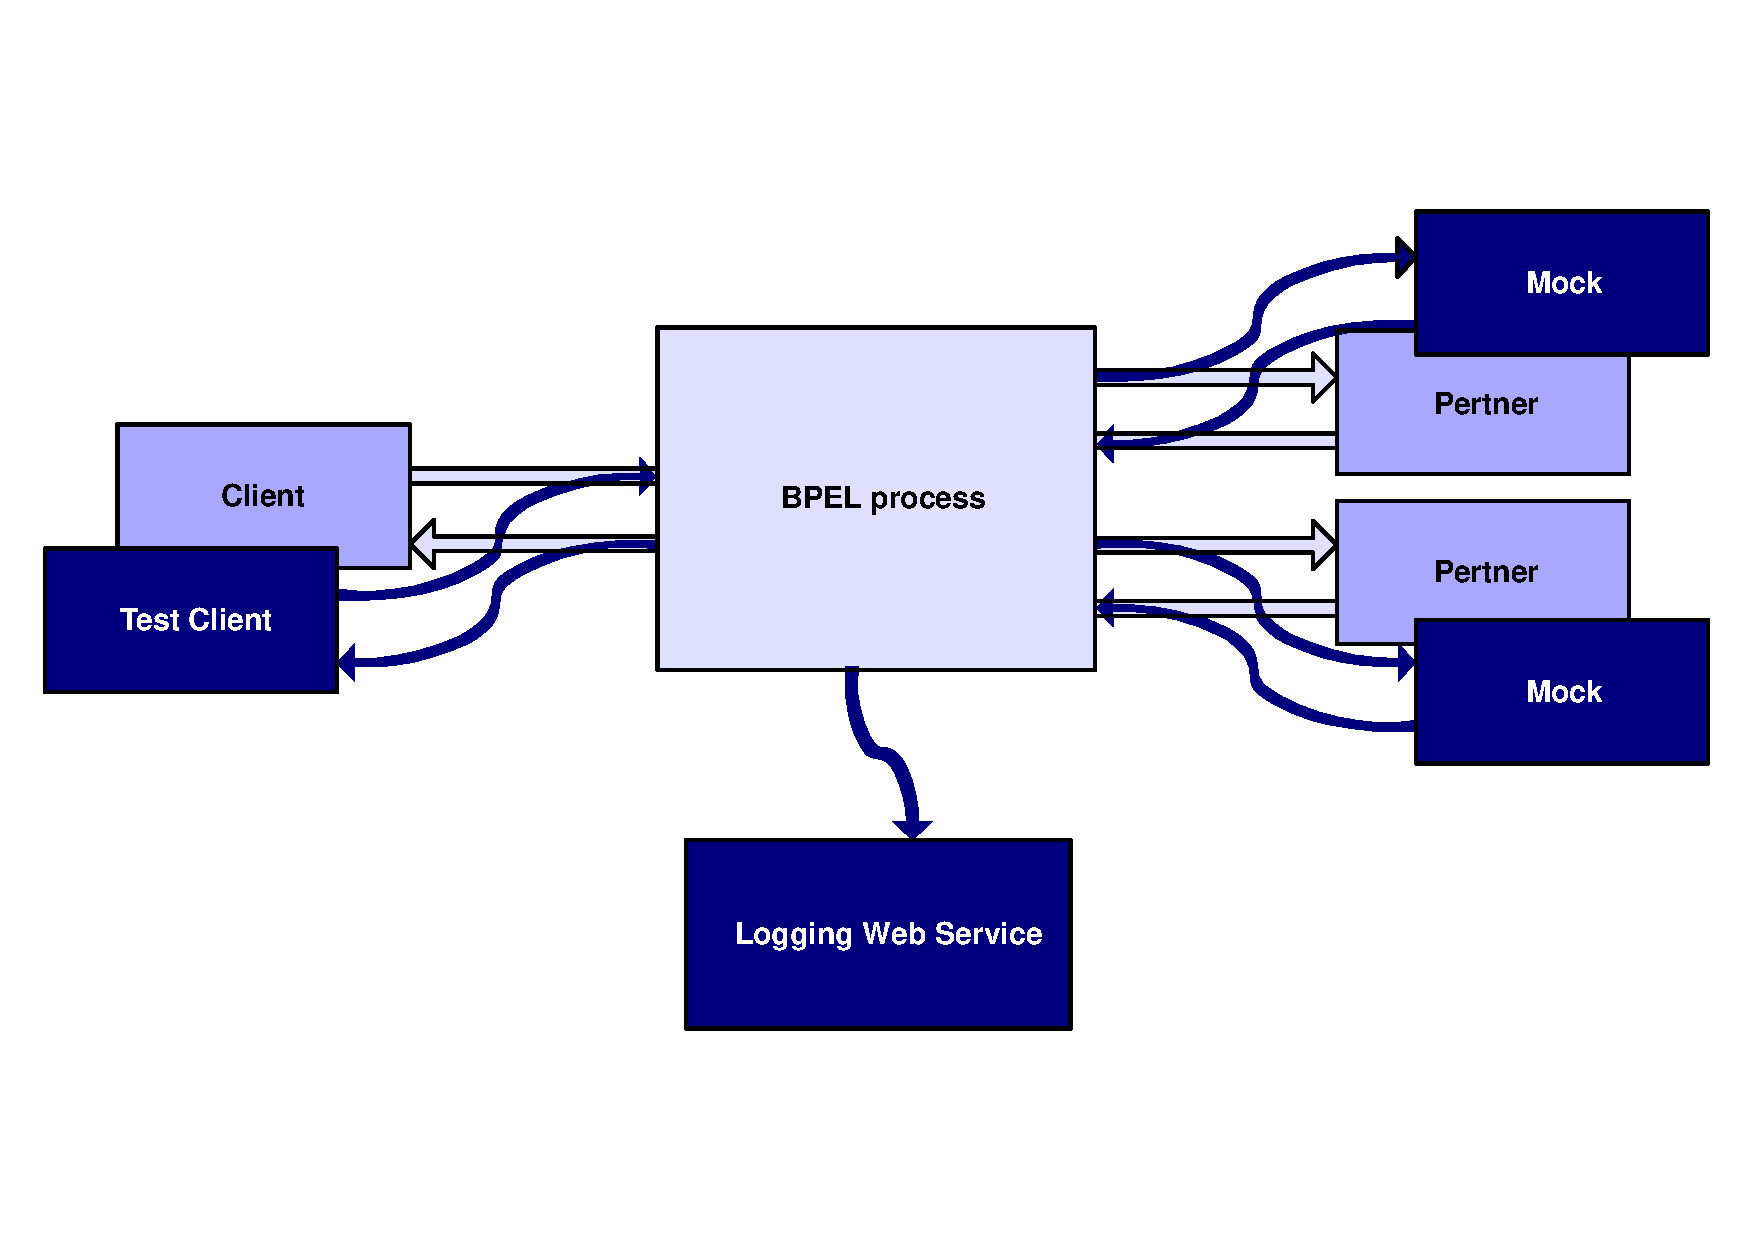
\includegraphics[width=0.90\textwidth]{bilder/loggingservice.pdf}
	\label{fig:loggingservice}
\end{figure}

\bibliographystyle{plain}
\bibliography{referenzen}
\end{document}